\SetHeaderColor{Part5Color}
\renewcommand{\CurrentPartColor}{Part5Color}
\cleardoublepage
\renewcommand{\CurrentPartNumber}{Partie 05}
\renewcommand{\CurrentPartName}{Les Munitions}
\renewcommand{\CurrentChapterType}{Chapitre}

\part{Munitions}

\markboth{Munitions}{Munitions}

    \chapter{Introduction aux munitions}
    \label{chap:introduction_munitions}
    %==============================================================================
% Chapitre 39 - Introduction aux munitions
%==============================================================================

\section{Introduction}

L'arme et le projectile ne constituent que deux éléments d'un système plus
vaste.

Pour qu'un tir puisse avoir lieu, il est nécessaire de disposer d'un ensemble
capable :

\begin{itemize}
    \item de contenir le projectile ;
    \item de stocker l'énergie nécessaire à son lancement ;
    \item d'initier la combustion ;
    \item d'assurer le bon fonctionnement de l'arme.
\end{itemize}

Cet ensemble est appelé munition.

\begin{aretenir}

La munition regroupe l'ensemble des éléments nécessaires au lancement d'un
projectile.

\end{aretenir}

\section{Définition}

Dans le langage courant, les termes \emph{munition}, \emph{cartouche} et
\emph{balle} sont parfois utilisés comme synonymes.

D'un point de vue technique, ces termes désignent pourtant des réalités
différentes.

\begin{itemize}
    \item La munition désigne l'ensemble complet.
    \item La cartouche est une forme particulière de munition.
    \item La balle est uniquement le projectile.
\end{itemize}

Cette distinction est importante pour éviter toute ambiguïté.

\section{Rôle de la munition}

La munition remplit plusieurs fonctions essentielles.

Elle doit :

\begin{itemize}
    \item stocker l'énergie propulsive ;
    \item protéger ses composants ;
    \item permettre le chargement de l'arme ;
    \item assurer une mise à feu fiable ;
    \item lancer le projectile dans des conditions reproductibles.
\end{itemize}

\section{Évolution historique}

Les premières armes à feu utilisaient des composants séparés :

\begin{itemize}
    \item poudre ;
    \item projectile ;
    \item système d'allumage.
\end{itemize}

Le tireur devait charger ces éléments individuellement.

Cette procédure était lente et source d'erreurs.

L'apparition de la cartouche moderne a profondément transformé l'emploi des
armes à feu.

\section{La cartouche moderne}

La plupart des armes modernes utilisent des cartouches métalliques.

Elles regroupent dans un ensemble unique :

\begin{itemize}
    \item l'étui ;
    \item l'amorce ;
    \item la poudre ;
    \item le projectile.
\end{itemize}

Cette architecture offre :

\begin{itemize}
    \item simplicité ;
    \item fiabilité ;
    \item sécurité ;
    \item rapidité de mise en œuvre.
\end{itemize}

\section{Les quatre éléments fondamentaux}

Une cartouche moderne est généralement constituée de quatre éléments
principaux :

\begin{enumerate}
    \item le projectile ;
    \item l'étui ;
    \item la charge propulsive ;
    \item l'amorce.
\end{enumerate}

Chacun de ces composants joue un rôle spécifique.

Les chapitres suivants les étudieront en détail.

\section{Le projectile}

Le projectile constitue la partie destinée à quitter l'arme.

Nous avons consacré toute la partie précédente à son étude.

Ses caractéristiques influencent notamment :

\begin{itemize}
    \item la portée ;
    \item la précision ;
    \item la stabilité ;
    \item les effets à l'impact.
\end{itemize}

\section{L'étui}

L'étui sert à regrouper les différents composants de la cartouche.

Il participe également :

\begin{itemize}
    \item au chargement ;
    \item à l'extraction ;
    \item à l'étanchéité des gaz.
\end{itemize}

Son rôle est souvent sous-estimé alors qu'il est essentiel au
fonctionnement de l'arme.

\section{La charge propulsive}

La charge propulsive est généralement constituée d'une poudre sans fumée.

Sa combustion produit :

\begin{itemize}
    \item des gaz ;
    \item de la chaleur ;
    \item de la pression.
\end{itemize}

Cette pression est à l'origine de l'accélération du projectile.

\section{L'amorce}

L'amorce constitue le système d'initiation.

Lorsqu'elle est percutée :

\begin{itemize}
    \item une réaction chimique se produit ;
    \item une flamme est générée ;
    \item la poudre est enflammée.
\end{itemize}

Elle représente le premier maillon de la chaîne du tir.

\section{Munition et système arme}

Une munition ne peut être étudiée indépendamment de l'arme.

Les caractéristiques des deux éléments doivent être compatibles.

On retrouve notamment des contraintes liées :

\begin{itemize}
    \item au calibre ;
    \item à la pression ;
    \item à la géométrie ;
    \item au fonctionnement mécanique.
\end{itemize}

\section{Performances balistiques}

La munition influence directement :

\begin{itemize}
    \item la vitesse initiale ;
    \item la précision ;
    \item l'énergie cinétique ;
    \item la portée ;
    \item le comportement terminal.
\end{itemize}

Deux projectiles identiques peuvent produire des résultats très différents
selon la munition utilisée.

\section{Normalisation}

Les munitions modernes sont généralement normalisées.

Des organismes spécialisés définissent notamment :

\begin{itemize}
    \item les dimensions ;
    \item les pressions admissibles ;
    \item les méthodes d'essai ;
    \item les critères de sécurité.
\end{itemize}

Cette normalisation favorise l'interchangeabilité et la sécurité.

\section{Sécurité}

Les munitions contiennent de l'énergie chimique.

Elles doivent être :

\begin{itemize}
    \item fabriquées ;
    \item transportées ;
    \item stockées ;
    \item utilisées
\end{itemize}

dans le respect de règles de sécurité adaptées.

\section{Pourquoi étudier les munitions ?}

La compréhension des munitions permet notamment de mieux comprendre :

\begin{itemize}
    \item la balistique intérieure ;
    \item les performances des armes ;
    \item les variations de vitesse ;
    \item certains incidents de tir ;
    \item les phénomènes de précision.
\end{itemize}

Les munitions constituent donc une composante fondamentale de toute étude
balistique.

\section{Organisation de cette partie}

Cette partie abordera successivement :

\begin{itemize}
    \item la structure des cartouches ;
    \item les étuis ;
    \item les amorces ;
    \item les poudres ;
    \item les calibres ;
    \item la fabrication ;
    \item le rechargement ;
    \item le stockage ;
    \item la sécurité.
\end{itemize}

Elle fournira les bases nécessaires à l'étude de la balistique intérieure.

\section{À retenir}

\begin{aretenir}

\begin{itemize}
    \item La munition fournit l'énergie nécessaire au lancement du
          projectile.
    \item Une cartouche moderne comprend généralement un projectile, un
          étui, une amorce et une charge propulsive.
    \item La munition constitue le lien entre l'arme et le projectile.
    \item Elle influence directement les performances balistiques.
    \item La compréhension des munitions est indispensable à l'étude de la
          balistique intérieure.
\end{itemize}

\end{aretenir}


    \chapter{Structure d'une cartouche}
    \label{chap:structure_cartouche}
    %==============================================================================
% Chapitre 40 - Structure d'une cartouche
%==============================================================================

\section{Introduction}

La cartouche moderne regroupe dans un ensemble unique tous les éléments
nécessaires au lancement d'un projectile.

Cette conception constitue l'une des innovations majeures de l'histoire des
armes à feu.

Elle permet :

\begin{itemize}
    \item un chargement rapide ;
    \item une excellente fiabilité ;
    \item une bonne protection des composants ;
    \item une grande reproductibilité des performances.
\end{itemize}

\begin{figure}[htbp]
\centering
\begin{tikzpicture}[scale=1]

% Etui
\draw[thick] (0,0) -- (0,5);
\draw[thick] (2,0) -- (2,5);
\draw[thick] (0,0) -- (2,0);

% Epaulement
\draw[thick] (0,5) -- (0.5,6);
\draw[thick] (2,5) -- (1.5,6);

% Collet
\draw[thick] (0.5,6) -- (0.5,7);
\draw[thick] (1.5,6) -- (1.5,7);

% Projectile
\draw[thick] (0.5,7) -- (1,8);
\draw[thick] (1.5,7) -- (1,8);

% Amorce
\draw[fill=white] (1,0) circle (0.2);

% Labels
\node[right] at (2.3,7.5) {Projectile};
\node[right] at (2.3,3.5) {Poudre};
\node[right] at (2.3,0.2) {Amorce};
\node[left] at (-0.3,3.5) {Étui};

\end{tikzpicture}
\caption{Structure simplifiée d'une cartouche à percussion centrale.}
\label{fig:cartouche_generale}
\end{figure}

\begin{aretenir}

Une cartouche moderne regroupe dans un même ensemble le projectile, l'étui,
la poudre et l'amorce.

\end{aretenir}

\section{Vue d'ensemble}

Une cartouche moderne est généralement constituée de quatre éléments
principaux :

\begin{enumerate}
    \item le projectile ;
    \item l'étui ;
    \item la charge propulsive ;
    \item l'amorce.
\end{enumerate}

Ces éléments fonctionnent ensemble pour produire le tir.

\section{Le projectile}

Le projectile est la seule partie destinée à quitter l'arme.

Son rôle est de transmettre l'énergie vers la cible.

Ses caractéristiques influencent notamment :

\begin{itemize}
    \item la précision ;
    \item la portée ;
    \item la stabilité ;
    \item les effets terminaux.
\end{itemize}

\section{L'étui}

L'étui constitue l'enveloppe de la cartouche.

Il remplit plusieurs fonctions :

\begin{itemize}
    \item maintien des composants ;
    \item protection de la poudre ;
    \item alimentation de l'arme ;
    \item étanchéité lors du tir.
\end{itemize}

\section{La charge propulsive}

La charge propulsive est généralement constituée d'une poudre sans fumée.

Sa combustion génère :

\begin{itemize}
    \item des gaz ;
    \item de la chaleur ;
    \item de la pression.
\end{itemize}

Cette pression accélère le projectile dans le canon.

\section{L'amorce}

L'amorce constitue le dispositif d'allumage.

Lorsqu'elle est frappée par le percuteur :

\begin{itemize}
    \item elle produit une flamme ;
    \item cette flamme enflamme la poudre ;
    \item la combustion débute.
\end{itemize}

\section{Fonctionnement général}

La séquence simplifiée d'un tir est la suivante :

\begin{enumerate}
    \item percussion de l'amorce ;
    \item inflammation de la poudre ;
    \item production de gaz ;
    \item augmentation de la pression ;
    \item mouvement du projectile ;
    \item sortie du projectile du canon.
\end{enumerate}

Cette séquence sera étudiée en détail dans la partie consacrée à la
balistique intérieure.

\section{Cartouche à percussion centrale}

La majorité des cartouches modernes utilisent une amorce située au centre du
culot.

On parle alors de percussion centrale.

Cette architecture présente :

\begin{itemize}
    \item une grande robustesse ;
    \item une bonne fiabilité ;
    \item une forte résistance à la pression.
\end{itemize}

\section{Cartouche à percussion annulaire}

Certaines cartouches utilisent une amorce répartie dans le bourrelet de
l'étui.

On parle alors de percussion annulaire.

Le cas le plus connu est celui du :

\begin{itemize}
    \item .22 Long Rifle.
\end{itemize}

Ces cartouches sont généralement destinées à des pressions plus faibles.

\section{Importance de l'assemblage}

Les performances d'une cartouche dépendent non seulement de ses composants,
mais également de leur assemblage.

Les paramètres importants incluent notamment :

\begin{itemize}
    \item la longueur totale ;
    \item le sertissage ;
    \item la masse de poudre ;
    \item l'enfoncement du projectile.
\end{itemize}

\section{Vers l'étude détaillée des composants}

La compréhension complète d'une cartouche nécessite maintenant l'étude de
chacun de ses éléments.

Nous commencerons par l'étui, composant souvent discret mais pourtant
essentiel au fonctionnement et à la sécurité du système.

\section{À retenir}

\begin{aretenir}

\begin{itemize}
    \item Une cartouche moderne comprend quatre éléments principaux.
    \item L'amorce initie le tir.
    \item La poudre fournit l'énergie.
    \item L'étui assure le maintien et l'étanchéité.
    \item Le projectile est la partie destinée à quitter l'arme.
\end{itemize}

\end{aretenir}


    \chapter{L'étui}
    \label{chap:etui}
    %==============================================================================
% Chapitre 41 - L'étui
%==============================================================================

\section{Introduction}

L'étui est l'élément central de la cartouche moderne.

Souvent considéré comme un simple contenant, il joue pourtant un rôle
fondamental dans :

\begin{itemize}
    \item le fonctionnement de l'arme ;
    \item la sécurité ;
    \item la fiabilité ;
    \item la précision.
\end{itemize}

Il assure le maintien des différents composants de la cartouche et participe
activement au déroulement du tir.

\begin{aretenir}

L'étui n'est pas un simple récipient : il constitue un composant mécanique
essentiel de la cartouche.

\end{aretenir}

\begin{figure}[htbp]
\centering
\begin{tikzpicture}[scale=1.2]

% Corps principal
\draw[thick] (0,0) -- (0,5);
\draw[thick] (2,0) -- (2,5);

% Épaulement
\draw[thick] (0,5) -- (0.5,6);
\draw[thick] (2,5) -- (1.5,6);

% Collet
\draw[thick] (0.5,6) -- (0.5,7);
\draw[thick] (1.5,6) -- (1.5,7);

% Projectile
\draw[thick] (0.5,7) -- (1,8);
\draw[thick] (1.5,7) -- (1,8);

% Culot
\draw[thick] (-0.2,0) -- (2.2,0);

% Amorce
\draw[fill=white] (1,0.25) circle (0.15);

% Annotations
\draw[->] (3,7.5) -- (1,7.6);
\node[right] at (3,7.5) {Projectile};

\draw[->] (3,6.3) -- (1.5,6.5);
\node[right] at (3,6.3) {Collet};

\draw[->] (3,5.3) -- (1.7,5.5);
\node[right] at (3,5.3) {Épaulement};

\draw[->] (3,3.5) -- (2,3.5);
\node[right] at (3,3.5) {Corps};

\draw[->] (3,0.7) -- (2,0.3);
\node[right] at (3,0.7) {Culot};

\draw[->] (-2,0.5) -- (1,0.25);
\node[left] at (-2,0.5) {Amorce};

\end{tikzpicture}
\caption{Principales parties d'un étui à gorge de type bottleneck.}
\label{fig:parties_etui}
\end{figure}

\section{Fonctions principales}

L'étui remplit plusieurs fonctions simultanément :

\begin{itemize}
    \item contenir la charge propulsive ;
    \item maintenir le projectile ;
    \item recevoir l'amorce ;
    \item permettre le chargement ;
    \item assurer l'étanchéité lors du tir ;
    \item faciliter l'extraction après le tir.
\end{itemize}

Chaque fonction influence directement le fonctionnement de l'arme.

\section{Évolution historique}

Les premières armes à feu ne possédaient pas d'étui métallique.

La poudre et le projectile étaient chargés séparément.

L'apparition des cartouches métalliques au XIX\ieme\ siècle a permis :

\begin{itemize}
    \item d'accélérer le chargement ;
    \item d'améliorer la fiabilité ;
    \item d'augmenter les cadences de tir ;
    \item de supporter des pressions plus élevées.
\end{itemize}

Cette innovation a profondément transformé les armes à feu.

\section{Constitution générale}

Un étui moderne comporte généralement plusieurs zones distinctes :

\begin{itemize}
    \item le collet ;
    \item l'épaulement ;
    \item le corps ;
    \item le culot ;
    \item la gorge d'extraction.
\end{itemize}

Chacune possède une fonction spécifique.

\section{Le collet}

Le collet est la partie supérieure de l'étui.

Il assure le maintien du projectile.

Sa géométrie influence notamment :

\begin{itemize}
    \item la tension de collet ;
    \item la régularité du départ du projectile ;
    \item la précision.
\end{itemize}

\section{L'épaulement}

L'épaulement relie le corps de l'étui au collet.

Dans de nombreuses cartouches modernes, il sert également de référence pour
le positionnement dans la chambre.

On parle alors de prise de feuillure sur l'épaulement.

\section{Le corps}

Le corps constitue la plus grande partie du volume de l'étui.

Il contient principalement :

\begin{itemize}
    \item la poudre ;
    \item les gaz produits lors du tir.
\end{itemize}

Sa capacité interne influence directement les performances balistiques.

\section{Le culot}

Le culot est la partie arrière de l'étui.

Il supporte les pressions les plus importantes lors du tir.

Cette zone doit présenter une résistance mécanique élevée.

Elle comporte généralement :

\begin{itemize}
    \item le logement d'amorce ;
    \item la gorge d'extraction ;
    \item éventuellement un bourrelet.
\end{itemize}

\section{La gorge d'extraction}

La gorge d'extraction permet à l'extracteur de saisir l'étui après le tir.

Elle joue un rôle essentiel dans le fonctionnement des armes à répétition et
semi-automatiques.

\section{Le bourrelet}

Certaines cartouches possèdent un bourrelet dépassant du diamètre du corps.

On parle alors de cartouches à bourrelet.

Exemples :

\begin{itemize}
    \item .22 Long Rifle ;
    \item .38 Special ;
    \item .357 Magnum.
\end{itemize}

D'autres cartouches sont dites sans bourrelet apparent (\emph{rimless}).

\section{Matériaux}

La majorité des étuis modernes sont fabriqués en laiton.

Ce matériau présente plusieurs avantages :

\begin{itemize}
    \item bonne résistance mécanique ;
    \item excellente ductilité ;
    \item bonne résistance à la corrosion ;
    \item facilité de fabrication.
\end{itemize}

D'autres matériaux existent :

\begin{itemize}
    \item acier ;
    \item aluminium ;
    \item polymères.
\end{itemize}

\section{L'obturation}

Lors du tir, la pression augmente rapidement.

L'étui se dilate alors contre les parois de la chambre.

Ce phénomène est appelé obturation.

Il permet :

\begin{itemize}
    \item d'empêcher la fuite des gaz vers l'arrière ;
    \item de protéger le tireur ;
    \item d'améliorer le rendement énergétique.
\end{itemize}

\begin{aretenir}

L'obturation est l'une des fonctions les plus importantes de l'étui.

\end{aretenir}

\section{Retour élastique}

Après le tir, la pression diminue.

L'étui se contracte légèrement grâce à son élasticité.

Cette contraction facilite son extraction.

C'est l'une des raisons du succès du laiton.

\section{Capacité interne}

La capacité interne correspond au volume disponible pour la poudre.

Cette grandeur influence :

\begin{itemize}
    \item la pression ;
    \item la vitesse initiale ;
    \item les performances globales.
\end{itemize}

Deux étuis extérieurement identiques peuvent présenter des capacités
internes différentes.

\section{Tolérances de fabrication}

Les dimensions d'un étui sont définies avec précision.

Les tolérances influencent notamment :

\begin{itemize}
    \item la sécurité ;
    \item la précision ;
    \item la compatibilité avec les chambres.
\end{itemize}

\section{Étuis et rechargement}

Les étuis métalliques peuvent souvent être réutilisés.

Le rechargement consiste notamment à :

\begin{itemize}
    \item désamorcer ;
    \item recalibrer ;
    \item réamorcer ;
    \item recharger en poudre ;
    \item replacer un projectile.
\end{itemize}

Cette pratique sera étudiée dans un chapitre dédié.

\section{Influence sur la précision}

La qualité de l'étui influence :

\begin{itemize}
    \item la régularité des pressions ;
    \item la vitesse initiale ;
    \item la dispersion des tirs.
\end{itemize}

Les tireurs de précision accordent donc une attention particulière à ce
composant.

\section{Vers les amorces}

L'étui constitue l'ossature de la cartouche.

Cependant, sans système d'allumage, aucun tir ne pourrait avoir lieu.

Nous allons maintenant étudier l'amorce, premier élément actif de la chaîne
de mise à feu.

\section{À retenir}

\begin{aretenir}

\begin{itemize}
    \item L'étui regroupe les composants de la cartouche.
    \item Il assure le chargement, l'obturation et l'extraction.
    \item Le laiton est le matériau le plus utilisé.
    \item La capacité interne influence les performances balistiques.
    \item La qualité de l'étui participe à la précision.
\end{itemize}

\end{aretenir}


    \chapter{Les amorces}
    \label{chap:amorces}
    %==============================================================================
% Chapitre 42 - Les amorces
%==============================================================================

\section{Introduction}

L'amorce constitue le dispositif d'initiation de la cartouche.

Son rôle est de transformer l'énergie mécanique apportée par le percuteur en
une énergie thermique capable d'enflammer la charge propulsive.

Bien que de très petite taille, elle joue un rôle fondamental dans la
fiabilité du tir.

\begin{aretenir}

L'amorce est le premier élément actif de la chaîne balistique.

\end{aretenir}

\section{Rôle de l'amorce}

L'amorce doit :

\begin{itemize}
    \item réagir à l'impact du percuteur ;
    \item produire une flamme ;
    \item transmettre cette flamme à la poudre ;
    \item fonctionner de manière fiable dans des conditions variées.
\end{itemize}

Son fonctionnement conditionne directement la mise à feu de la cartouche.

\section{Principe de fonctionnement}

Lors du tir :

\begin{enumerate}
    \item le percuteur frappe l'amorce ;
    \item le mélange détonant est comprimé ;
    \item une réaction chimique se produit ;
    \item une flamme est générée ;
    \item la poudre est enflammée.
\end{enumerate}

L'ensemble de cette séquence se déroule en une fraction de milliseconde.

\section{Constitution générale}

Une amorce moderne comprend généralement :

\begin{itemize}
    \item une coupelle métallique ;
    \item un mélange pyrotechnique ;
    \item une enclume ;
    \item un opercule éventuel selon les modèles.
\end{itemize}

Ces éléments sont assemblés avec une grande précision.

\section{La coupelle}

La coupelle constitue l'enveloppe métallique de l'amorce.

Elle doit :

\begin{itemize}
    \item résister à la manipulation ;
    \item se déformer sous l'action du percuteur ;
    \item contenir les produits de réaction.
\end{itemize}

Sa dureté influence le comportement de l'amorce.

\section{L'enclume}

L'enclume est une petite pièce métallique située à l'intérieur de l'amorce.

Lors de la percussion :

\begin{itemize}
    \item le mélange détonant est écrasé entre la coupelle et l'enclume ;
    \item la réaction est initiée.
\end{itemize}

Elle joue donc un rôle essentiel dans le déclenchement.

\section{Le mélange amorçant}

Le mélange amorçant est constitué de substances chimiques sensibles aux
chocs.

Il doit :

\begin{itemize}
    \item s'enflammer rapidement ;
    \item produire une température élevée ;
    \item générer une flamme suffisante pour allumer la poudre.
\end{itemize}

Sa composition a fortement évolué au cours de l'histoire.

\section{Évolution historique}

Les premières amorces utilisaient souvent des composés contenant du mercure.

Ces formulations présentaient plusieurs inconvénients :

\begin{itemize}
    \item corrosion ;
    \item vieillissement ;
    \item détérioration des étuis.
\end{itemize}

Les compositions modernes sont généralement plus sûres et plus stables.

\section{Amorces corrosives}

Certaines munitions anciennes utilisent des amorces dites corrosives.

Après le tir, elles laissent des résidus pouvant favoriser la corrosion des
armes.

Un nettoyage adapté est alors indispensable.

\section{Amorces non corrosives}

Les amorces modernes sont généralement non corrosives.

Elles ont progressivement remplacé les formulations anciennes dans la
plupart des applications civiles et militaires.

\section{Percussion centrale}

Dans les cartouches à percussion centrale :

\begin{itemize}
    \item l'amorce est placée au centre du culot ;
    \item le percuteur frappe directement cette zone.
\end{itemize}

Cette architecture est aujourd'hui la plus répandue.

\section{Percussion annulaire}

Dans les cartouches à percussion annulaire :

\begin{itemize}
    \item le mélange amorçant est réparti dans le bourrelet ;
    \item le percuteur écrase le bord de l'étui.
\end{itemize}

Le .22 Long Rifle constitue l'exemple le plus connu.

\section{Dimensions}

Les amorces existent en plusieurs dimensions.

On rencontre notamment :

\begin{itemize}
    \item Small Pistol ;
    \item Large Pistol ;
    \item Small Rifle ;
    \item Large Rifle.
\end{itemize}

Le choix dépend de la cartouche concernée.

\section{Énergie d'allumage}

Toutes les amorces ne produisent pas la même énergie.

Certaines génèrent :

\begin{itemize}
    \item une flamme plus chaude ;
    \item une flamme plus longue ;
    \item une pression initiale plus importante.
\end{itemize}

Ces différences peuvent influencer la régularité des vitesses.

\section{Amorces Magnum}

Les amorces Magnum produisent généralement une flamme plus énergique.

Elles sont souvent utilisées :

\begin{itemize}
    \item avec des charges importantes ;
    \item avec certaines poudres lentes ;
    \item par temps froid.
\end{itemize}

Leur emploi doit rester cohérent avec les données de chargement.

\section{Influence sur la précision}

L'amorce influence directement :

\begin{itemize}
    \item la régularité de l'allumage ;
    \item la vitesse initiale ;
    \item les écarts de vitesse ;
    \item la précision finale.
\end{itemize}

Cette influence est parfois sous-estimée.

\section{Incidents liés aux amorces}

Plusieurs incidents peuvent être observés :

\begin{itemize}
    \item raté de percussion ;
    \item départ retardé ;
    \item amorce percée ;
    \item amorce soufflée.
\end{itemize}

L'analyse de ces phénomènes fournit souvent des informations utiles sur le
fonctionnement de la cartouche ou de l'arme.

\section{Vers les poudres propulsives}

L'amorce ne fournit qu'une faible quantité d'énergie.

Son rôle consiste uniquement à initier la combustion.

L'énergie principale du tir provient de la charge propulsive que nous allons
étudier dans le chapitre suivant.

\section{À retenir}

\begin{aretenir}

\begin{itemize}
    \item L'amorce initie le tir.
    \item Elle transforme un choc mécanique en flamme.
    \item Les amorces modernes sont généralement à percussion centrale.
    \item Leur régularité influence les performances balistiques.
    \item Elles constituent le premier maillon de la chaîne de mise à feu.
\end{itemize}

\end{aretenir}


    \chapter{Les poudres propulsives}
    \label{chap:poudres_propulsives}
    %==============================================================================
% Chapitre 43 - Les poudres propulsives
%==============================================================================

\section{Introduction}

La poudre propulsive constitue la source principale d'énergie d'une
cartouche.

Sa combustion produit les gaz nécessaires à l'accélération du projectile
dans le canon.

Les poudres modernes représentent l'aboutissement de plusieurs siècles
d'évolution technologique.

\begin{aretenir}

La poudre propulsive transforme son énergie chimique en énergie mécanique
par l'intermédiaire des gaz produits lors de sa combustion.

\end{aretenir}

\section{Rôle de la poudre}

La poudre doit :

\begin{itemize}
    \item s'enflammer rapidement ;
    \item brûler de manière contrôlée ;
    \item produire une quantité importante de gaz ;
    \item générer une pression adaptée ;
    \item assurer une vitesse initiale régulière.
\end{itemize}

Son comportement influence directement les performances balistiques.

\section{Un point de vocabulaire}

Contrairement à une idée répandue, la poudre d'une cartouche moderne
n'explose généralement pas.

Elle brûle très rapidement.

On parle de combustion rapide ou de déflagration.

Cette distinction est fondamentale.

\begin{aretenir}

La poudre propulsive déflagre ; elle ne détonne pas.

\end{aretenir}

\begin{figure}[htbp]
\centering

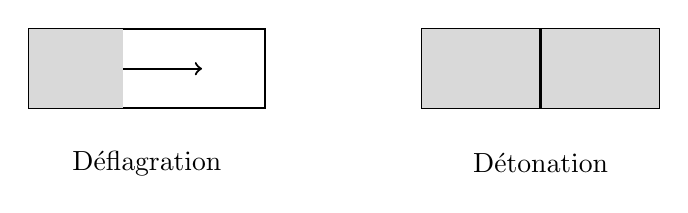
\begin{tikzpicture}[scale=1]

% Déflagration
\draw[thick] (0,0) rectangle (3,1);

\fill[gray!30] (0,0) rectangle (1.2,1);

\draw[->,thick] (1.2,0.5) -- (2.2,0.5);

\node at (1.5,-0.7) {Déflagration};

% Détonation
\draw[thick] (5,0) rectangle (8,1);

\fill[gray!30] (5,0) rectangle (8,1);

\draw[very thick] (6.5,0) -- (6.5,1);

\node at (6.5,-0.7) {Détonation};

\end{tikzpicture}

\caption{Illustration simplifiée d'une déflagration et d'une détonation.}
\label{fig:deflagration_detonation}
\end{figure}

\section{La poudre noire}

Pendant plusieurs siècles, les armes à feu ont utilisé la poudre noire.

Elle est traditionnellement constituée :

\begin{itemize}
    \item de nitrate de potassium ;
    \item de charbon ;
    \item de soufre.
\end{itemize}

Son utilisation a marqué l'histoire des armes à feu.

\section{Limites de la poudre noire}

La poudre noire présente plusieurs inconvénients :

\begin{itemize}
    \item production importante de fumée ;
    \item encrassement élevé ;
    \item rendement énergétique limité ;
    \item forte sensibilité à l'humidité.
\end{itemize}

Ces limitations ont conduit au développement de poudres plus performantes.

\section{Les poudres sans fumée}

La majorité des munitions modernes utilisent des poudres sans fumée.

Leur développement à la fin du XIX\ieme\ siècle a profondément transformé la
balistique.

Leurs avantages incluent :

\begin{itemize}
    \item une énergie plus élevée ;
    \item moins de résidus ;
    \item une meilleure régularité ;
    \item une réduction importante de la fumée.
\end{itemize}

\section{La nitrocellulose}

La nitrocellulose constitue le principal composant des poudres modernes.

Cette substance possède une forte capacité énergétique tout en restant
suffisamment stable pour être utilisée comme propulsif.

Elle est parfois appelée coton-poudre.

\section{Poudres simple base}

Les poudres dites simple base sont principalement constituées de
nitrocellulose.

Elles présentent généralement :

\begin{itemize}
    \item une bonne stabilité ;
    \item une combustion régulière ;
    \item une fabrication relativement simple.
\end{itemize}

\section{Poudres double base}

Les poudres double base contiennent généralement :

\begin{itemize}
    \item de la nitrocellulose ;
    \item de la nitroglycérine.
\end{itemize}

L'ajout de nitroglycérine augmente l'énergie disponible.

\section{Poudres triple base}

Certaines applications militaires utilisent des poudres triple base.

Celles-ci peuvent notamment contenir :

\begin{itemize}
    \item de la nitrocellulose ;
    \item de la nitroglycérine ;
    \item de la nitroguanidine.
\end{itemize}

Ces formulations sont principalement rencontrées dans les systèmes de gros
calibre.

\section{Formes des grains}

Les poudres propulsives existent sous différentes formes.

On rencontre notamment :

\begin{itemize}
    \item des grains sphériques ;
    \item des paillettes ;
    \item des bâtonnets ;
    \item des tubes perforés.
\end{itemize}

La géométrie influence fortement la combustion.

\begin{figure}[htbp]
\centering
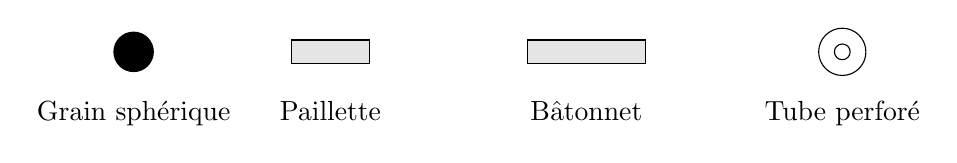
\begin{tikzpicture}[scale=1]

% Grain sphérique
\filldraw (0,0) circle (0.25);
\node[below] at (0,-0.5) {Grain sphérique};

% Paillette
\draw[fill=gray!20] (2,-0.15) rectangle (3,0.15);
\node[below] at (2.5,-0.5) {Paillette};

% Bâtonnet
\draw[fill=gray!20] (5,-0.15) rectangle (6.5,0.15);
\node[below] at (5.75,-0.5) {Bâtonnet};

% Tube perforé
\draw (9,0) circle (0.3);
\draw (9,0) circle (0.1);
\node[below] at (9,-0.5) {Tube perforé};

\end{tikzpicture}
\caption{Exemples de formes de grains utilisées dans les poudres propulsives.}
\label{fig:formes_grains}
\end{figure}

\section{Surface de combustion}

La vitesse de combustion dépend notamment de la surface exposée.

Lorsque la surface évolue pendant la combustion :

\begin{itemize}
    \item la production de gaz évolue ;
    \item la pression évolue ;
    \item les performances changent.
\end{itemize}

La forme des grains est donc un paramètre essentiel.

\begin{figure}[htbp]
\centering

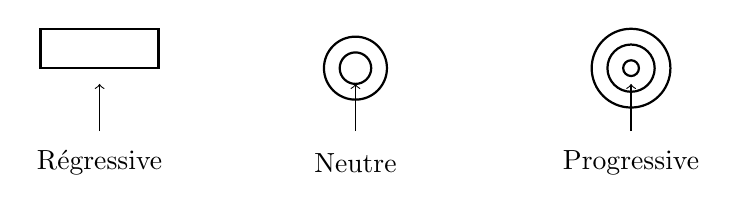
\begin{tikzpicture}[scale=1]

% Régressive
\draw[thick] (0,0) rectangle (1.5,0.5);
\draw[->] (0.75,-0.8) -- (0.75,-0.2);
\node at (0.75,-1.2) {Régressive};

% Neutre
\draw[thick] (4,0) circle (0.4);
\draw[thick] (4,0) circle (0.2);
\draw[->] (4,-0.8) -- (4,-0.2);
\node at (4,-1.2) {Neutre};

% Progressive
\draw[thick] (7.5,0) circle (0.5);
\draw[thick] (7.5,0) circle (0.3);
\draw[thick] (7.5,0) circle (0.1);
\draw[->] (7.5,-0.8) -- (7.5,-0.2);
\node at (7.5,-1.2) {Progressive};

\end{tikzpicture}

\caption{Influence de la géométrie des grains sur l'évolution de la surface de combustion.}
\label{fig:surface_combustion}
\end{figure}

\section{Combustion progressive}

Certaines poudres sont conçues pour présenter une combustion progressive.

Au cours de la combustion :

\begin{itemize}
    \item la surface disponible augmente ;
    \item la production de gaz reste importante ;
    \item l'accélération du projectile est prolongée.
\end{itemize}

Ces poudres sont particulièrement adaptées aux armes à canon long.

\section{Combustion régressive}

Dans d'autres cas :

\begin{itemize}
    \item la surface diminue progressivement ;
    \item la production de gaz décroît ;
    \item la pression chute plus rapidement.
\end{itemize}

\section{Vivacité}

La vivacité caractérise la rapidité de combustion d'une poudre.

Une poudre vive :

\begin{itemize}
    \item brûle rapidement ;
    \item produit rapidement sa pression maximale.
\end{itemize}

Une poudre lente :

\begin{itemize}
    \item brûle plus progressivement ;
    \item maintient la pression plus longtemps.
\end{itemize}

\section{Choix de la poudre}

Le choix d'une poudre dépend notamment :

\begin{itemize}
    \item du calibre ;
    \item de la masse du projectile ;
    \item de la longueur du canon ;
    \item des performances recherchées.
\end{itemize}

Une poudre inadaptée peut dégrader les performances ou provoquer des
surpressions dangereuses.

\begin{figure}[htbp]
\centering

\begin{tikzpicture}[scale=1]

\draw[->] (0,0) -- (8,0) node[right] {Temps};

\draw[->] (0,0) -- (0,5) node[above] {Pression};

% Poudre vive
\draw[thick]
(0,0)
.. controls (0.8,4.5) and (1.5,4) ..
(3,0);

\node at (1.8,4.2) {Poudre vive};

% Poudre lente
\draw[thick]
(0,0)
.. controls (2,2.5) and (4.5,3.5) ..
(7,0);

\node at (5.5,3.0) {Poudre lente};

\end{tikzpicture}

\caption{Évolution simplifiée de la pression pour une poudre vive et une poudre lente.}
\label{fig:vivacite_poudre}
\end{figure}

\section{Température}

La température influence le comportement des poudres.

Elle peut modifier :

\begin{itemize}
    \item la vitesse de combustion ;
    \item la pression maximale ;
    \item la vitesse initiale.
\end{itemize}

Certaines poudres sont spécialement formulées pour limiter cette sensibilité.

\section{Vieillissement}

Les poudres évoluent lentement au cours du temps.

Leur stabilité dépend notamment :

\begin{itemize}
    \item des conditions de stockage ;
    \item de la température ;
    \item de l'humidité ;
    \item de leur composition chimique.
\end{itemize}

\section{Sécurité}

Les poudres propulsives doivent être manipulées avec précaution.

Elles contiennent une quantité importante d'énergie chimique.

Le respect des procédures de stockage et de manipulation est essentiel.

\section{Vers la balistique intérieure}

La poudre constitue la source d'énergie du tir.

Cependant, ce n'est qu'au moment de sa combustion que cette énergie est
transformée en pression puis en mouvement.

Nous étudierons ce processus en détail dans la partie consacrée à la
balistique intérieure.

\section{À retenir}

\begin{aretenir}

\begin{itemize}
    \item La poudre propulsive constitue la source d'énergie du tir.
    \item Les poudres modernes sont principalement à base de
          nitrocellulose.
    \item La forme des grains influence la combustion.
    \item La vivacité caractérise la rapidité de combustion.
    \item La poudre déflagre et ne détonne pas.
\end{itemize}

\end{aretenir}


    \chapter{Le projectile dans la cartouches}
    \label{chap:projectile_cartouche}
    %==============================================================================
% Chapitre 44 - Le projectile dans la cartouche
%==============================================================================

\section{Introduction}

Le projectile constitue l'élément destiné à quitter l'arme et à atteindre la
cible.

Cependant, avant son départ, il fait partie intégrante de la cartouche.

Sa position, son maintien et son assemblage influencent directement les
performances balistiques.

\begin{aretenir}

Le comportement d'un projectile dépend non seulement de sa géométrie mais
également de la manière dont il est assemblé dans la cartouche.

\end{aretenir}

\section{Le projectile dans la chaîne balistique}

Nous avons déjà étudié en détail :

\begin{itemize}
    \item la géométrie ;
    \item la masse ;
    \item la stabilité ;
    \item les propriétés aérodynamiques.
\end{itemize}

Dans ce chapitre, nous nous intéressons à son intégration dans la munition.

\section{Position dans l'étui}

Le projectile est maintenu dans le collet de l'étui.

Une partie du projectile demeure à l'intérieur de l'étui tandis qu'une autre
reste visible à l'extérieur.

Cette position influence directement :

\begin{itemize}
    \item la longueur totale de la cartouche ;
    \item le volume disponible pour la poudre ;
    \item l'alimentation de l'arme.
\end{itemize}

\section{Longueur totale}

La longueur totale de cartouche est souvent désignée par l'acronyme anglais :

\begin{quote}
OAL (\emph{Overall Length})
\end{quote}

ou :

\begin{quote}
COL (\emph{Cartridge Overall Length})
\end{quote}

Cette dimension joue un rôle essentiel dans le fonctionnement des armes.

\section{Importance de la longueur totale}

Une longueur incorrecte peut provoquer :

\begin{itemize}
    \item des incidents d'alimentation ;
    \item des problèmes de chambrage ;
    \item des variations de pression ;
    \item une dégradation de la précision.
\end{itemize}

Les fabricants définissent donc des limites précises.

\section{Enfoncement du projectile}

L'enfoncement correspond à la profondeur d'insertion du projectile dans
l'étui.

Cette grandeur influence directement :

\begin{itemize}
    \item le volume interne disponible ;
    \item la pression maximale ;
    \item la combustion de la poudre.
\end{itemize}

\begin{figure}[htbp]
\centering

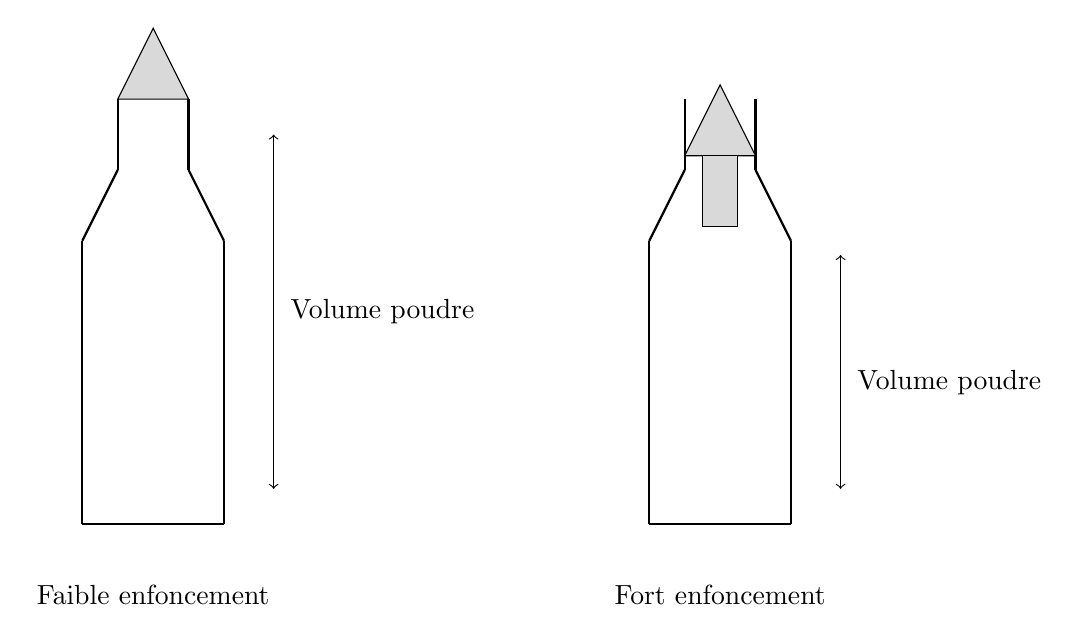
\begin{tikzpicture}[scale=0.9]

% Cartouche gauche
\draw[thick] (0,0) -- (0,4);
\draw[thick] (2,0) -- (2,4);
\draw[thick] (0,0) -- (2,0);

\draw[thick] (0,4) -- (0.5,5);
\draw[thick] (2,4) -- (1.5,5);

\draw[thick] (0.5,5) -- (0.5,6);
\draw[thick] (1.5,5) -- (1.5,6);

% Projectile peu enfoncé
\draw[fill=gray!30] (0.5,6) -- (1,7) -- (1.5,6) -- cycle;

\node at (1,-1) {Faible enfoncement};

% Flèche volume
\draw[<->] (2.7,0.5) -- (2.7,5.5);
\node[right] at (2.8,3) {Volume poudre};

% Cartouche droite
\begin{scope}[xshift=8cm]

\draw[thick] (0,0) -- (0,4);
\draw[thick] (2,0) -- (2,4);
\draw[thick] (0,0) -- (2,0);

\draw[thick] (0,4) -- (0.5,5);
\draw[thick] (2,4) -- (1.5,5);

\draw[thick] (0.5,5) -- (0.5,6);
\draw[thick] (1.5,5) -- (1.5,6);

% Projectile fortement enfoncé
\draw[fill=gray!30]
(0.5,5.2) --
(1,6.2) --
(1.5,5.2) --
cycle;

\draw[fill=gray!30]
(0.75,4.2)
rectangle
(1.25,5.2);

\node at (1,-1) {Fort enfoncement};

\draw[<->] (2.7,0.5) -- (2.7,3.8);
\node[right] at (2.8,2) {Volume poudre};

\end{scope}

\end{tikzpicture}

\caption{Influence de l'enfoncement du projectile sur le volume disponible pour la poudre.}
\label{fig:enfoncement_volume}
\end{figure}

\section{Volume disponible}

Lorsque l'enfoncement augmente :

\begin{itemize}
    \item le volume interne diminue ;
    \item la densité de chargement augmente ;
    \item la pression peut augmenter.
\end{itemize}

Cette relation est particulièrement importante en rechargement.

\begin{attention}

Une modification importante de l'enfoncement peut entraîner des variations
significatives de pression.

\end{attention}

\section{Maintien du projectile}

Le projectile doit être maintenu fermement dans le collet.

Ce maintien doit être suffisant pour :

\begin{itemize}
    \item résister aux manipulations ;
    \item supporter le recul ;
    \item garantir une mise à feu régulière.
\end{itemize}

\section{Tension de collet}

La tension de collet correspond à l'effort exercé par le collet sur le
projectile.

Elle dépend notamment :

\begin{itemize}
    \item du diamètre du projectile ;
    \item des dimensions du collet ;
    \item des propriétés mécaniques de l'étui.
\end{itemize}

\section{Influence sur la précision}

Une tension de collet régulière contribue à :

\begin{itemize}
    \item une combustion plus homogène ;
    \item une meilleure régularité des vitesses ;
    \item une meilleure précision.
\end{itemize}

\section{Alignement}

Le projectile doit être correctement aligné avec l'axe de l'étui.

Un mauvais alignement peut entraîner :

\begin{itemize}
    \item une entrée asymétrique dans les rayures ;
    \item une augmentation de la dispersion ;
    \item une perte de précision.
\end{itemize}

\section{Distance aux rayures}

Une fois chambrée, la cartouche positionne le projectile à une certaine
distance des rayures.

Cette distance est parfois appelée :

\begin{quote}
\emph{jump}
\end{quote}

dans la littérature anglo-saxonne.

\section{Influence du jump}

Le jump influence notamment :

\begin{itemize}
    \item la pression ;
    \item la précision ;
    \item le comportement du projectile au départ du coup.
\end{itemize}

Son optimisation constitue un sujet important en rechargement de précision.

\begin{figure}[htbp]
\centering

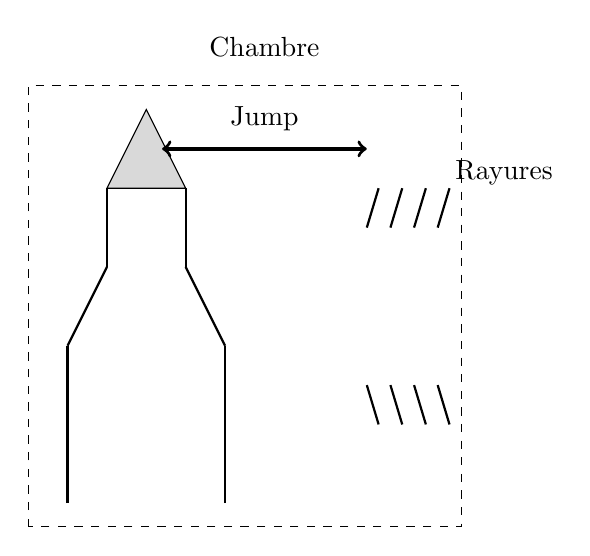
\begin{tikzpicture}[scale=1]

% Cartouche
\draw[thick] (0,0) -- (0,2);
\draw[thick] (2,0) -- (2,2);

\draw[thick] (0,2) -- (0.5,3);
\draw[thick] (2,2) -- (1.5,3);

\draw[thick] (0.5,3) -- (0.5,4);
\draw[thick] (1.5,3) -- (1.5,4);

% Projectile
\draw[fill=gray!30]
(0.5,4) --
(1,5) --
(1.5,4) --
cycle;

% Chambre
\draw[dashed] (-0.5,-0.3) rectangle (5,5.3);

\node at (2.5,5.8) {Chambre};

% Rayures
\foreach \x in {3.8,4.1,4.4,4.7}
{
    \draw[thick]
    (\x,3.5) --
    (\x+0.15,4.0);

    \draw[thick]
    (\x,1.5) --
    (\x+0.15,1.0);
}

\node[right] at (4.8,4.2) {Rayures};

% Flèche Jump
\draw[<->,very thick]
(1.2,4.5) --
(3.8,4.5);

\node[above] at (2.5,4.6) {Jump};

\end{tikzpicture}

\caption{Distance entre le projectile et les rayures lorsque la cartouche est chambrée.}
\label{fig:jump}
\end{figure}

\section{Projectiles sertis et non sertis}

Certaines cartouches utilisent un sertissage du projectile.

D'autres reposent uniquement sur la tension de collet.

Le choix dépend :

\begin{itemize}
    \item du type de munition ;
    \item du mode d'alimentation ;
    \item des contraintes mécaniques.
\end{itemize}

\section{Influence du recul}

Dans certaines armes, le recul peut provoquer un déplacement du projectile à
l'intérieur de l'étui.

Le maintien doit être suffisant pour éviter ce phénomène.

\section{Influence sur la balistique intérieure}

Le projectile participe directement à la balistique intérieure.

Sa masse et sa résistance au mouvement influencent :

\begin{itemize}
    \item la montée en pression ;
    \item la combustion ;
    \item la vitesse initiale.
\end{itemize}

\section{Vers le sertissage}

Le maintien du projectile peut être renforcé par une opération spécifique :

le sertissage.

Cette opération fera l'objet du chapitre suivant.

\section{À retenir}

\begin{aretenir}

\begin{itemize}
    \item Le projectile est maintenu dans le collet de l'étui.
    \item Son enfoncement influence directement la pression.
    \item La longueur totale de cartouche est une dimension critique.
    \item La tension de collet participe à la régularité du tir.
    \item L'alignement du projectile influence la précision.
\end{itemize}

\end{aretenir}


    \chapter{Le sertissage}
    \label{chap:sertissage}
    %==============================================================================
% Chapitre 45 - Le sertissage
%==============================================================================

\section{Introduction}

Le projectile est généralement maintenu dans le collet de l'étui par la seule
tension exercée par celui-ci.

Dans certaines situations, ce maintien peut être renforcé par une opération
appelée sertissage.

Le sertissage constitue une étape importante dans la fabrication de nombreuses
munitions.

\begin{aretenir}

Le sertissage consiste à déformer légèrement le collet afin d'améliorer le
maintien du projectile.

\end{aretenir}

\section{Objectifs du sertissage}

Le sertissage peut remplir plusieurs fonctions :

\begin{itemize}
    \item empêcher le déplacement du projectile ;
    \item améliorer la résistance aux chocs ;
    \item résister aux effets du recul ;
    \item améliorer la régularité du départ du projectile ;
    \item faciliter le fonctionnement de certaines armes.
\end{itemize}

Selon les applications, l'importance de ces fonctions varie.

\section{Pourquoi maintenir le projectile ?}

Avant le tir, le projectile est soumis à diverses contraintes :

\begin{itemize}
    \item manipulations ;
    \item vibrations ;
    \item chocs ;
    \item accélérations ;
    \item recul.
\end{itemize}

Un maintien insuffisant peut provoquer des déplacements indésirables.

\section{Déplacement vers l'intérieur}

Dans certains cas, le projectile peut s'enfoncer davantage dans l'étui.

Ce phénomène réduit le volume disponible pour la poudre.

Il peut alors entraîner :

\begin{itemize}
    \item une augmentation de la pression ;
    \item une modification des performances ;
    \item des risques de surpression.
\end{itemize}

\section{Déplacement vers l'extérieur}

Le projectile peut également sortir partiellement de l'étui.

Ce phénomène est particulièrement redouté dans certains revolvers puissants.

Une cartouche trop longue peut alors :

\begin{itemize}
    \item gêner la rotation du barillet ;
    \item provoquer un incident de fonctionnement.
\end{itemize}

\section{Principe du sertissage}

Le sertissage consiste à déformer légèrement le collet autour du projectile.

Cette déformation augmente l'effort nécessaire pour déplacer celui-ci.

Le maintien devient alors plus important.

\section{Sertissage et tension de collet}

Le sertissage ne remplace pas une bonne tension de collet.

Dans la plupart des cas :

\begin{itemize}
    \item la tension de collet assure l'essentiel du maintien ;
    \item le sertissage constitue un complément.
\end{itemize}

\begin{aretenir}

Un sertissage ne doit pas compenser un collet mal dimensionné.

\end{aretenir}

\begin{figure}[htbp]
\centering

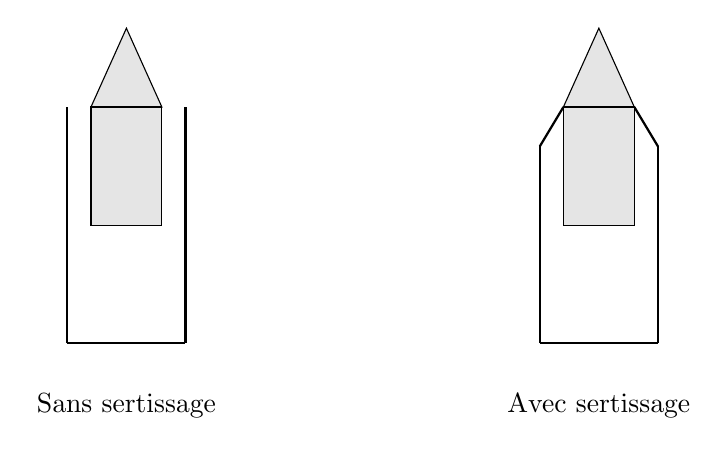
\begin{tikzpicture}[scale=1]

% Sans sertissage
\begin{scope}

\draw[thick] (0,0) -- (0,3);
\draw[thick] (1.5,0) -- (1.5,3);

\draw[thick] (0,0) -- (1.5,0);

% Projectile
\draw[fill=gray!20]
(0.3,3) --
(0.75,4) --
(1.2,3) --
cycle;

\draw[fill=gray!20]
(0.3,1.5) rectangle (1.2,3);

\node at (0.75,-0.8) {Sans sertissage};

\end{scope}

% Avec sertissage
\begin{scope}[xshift=6cm]

\draw[thick] (0,0) -- (0,2.5);
\draw[thick] (1.5,0) -- (1.5,2.5);

\draw[thick] (0,0) -- (1.5,0);

% Collet replié
\draw[thick] (0,2.5) -- (0.3,3);
\draw[thick] (1.5,2.5) -- (1.2,3);

% Projectile
\draw[fill=gray!20]
(0.3,3) --
(0.75,4) --
(1.2,3) --
cycle;

\draw[fill=gray!20]
(0.3,1.5) rectangle (1.2,3);

\node at (0.75,-0.8) {Avec sertissage};

\end{scope}

\end{tikzpicture}

\caption{Influence du sertissage sur le maintien du projectile dans le collet.}
\label{fig:sertissage_principe}

\end{figure}

\section{Le sertissage roulé}

Le sertissage roulé (\emph{roll crimp}) consiste à rabattre légèrement le bord
du collet vers l'intérieur.

Cette technique est fréquemment utilisée pour :

\begin{itemize}
    \item les munitions de revolver ;
    \item certaines cartouches de chasse ;
    \item certaines cartouches à fort recul.
\end{itemize}

\section{Le sertissage conique}

Le sertissage conique (\emph{taper crimp}) réduit progressivement le diamètre
du collet.

Cette méthode est couramment utilisée pour :

\begin{itemize}
    \item les cartouches d'armes de poing modernes ;
    \item les cartouches prenant leur feuillure sur le collet.
\end{itemize}

\begin{figure}[htbp]
\centering

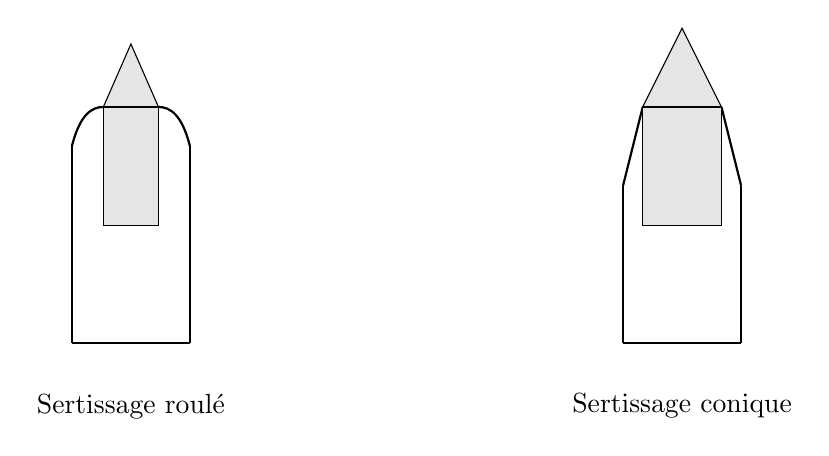
\begin{tikzpicture}[scale=1]

% Roll Crimp
\begin{scope}

\draw[thick] (0,0) -- (0,2.5);
\draw[thick] (1.5,0) -- (1.5,2.5);

\draw[thick] (0,0) -- (1.5,0);

% Repli du collet
\draw[thick]
(0,2.5)
.. controls (0.1,2.9) and (0.25,3.0) ..
(0.4,3.0);

\draw[thick]
(1.5,2.5)
.. controls (1.4,2.9) and (1.25,3.0) ..
(1.1,3.0);

% Projectile
\draw[fill=gray!20]
(0.4,3) --
(0.75,3.8) --
(1.1,3) --
cycle;

\draw[fill=gray!20]
(0.4,1.5) rectangle (1.1,3);

\node at (0.75,-0.8) {Sertissage roulé};

\end{scope}

% Taper Crimp
\begin{scope}[xshift=7cm]

\draw[thick] (0,0) -- (0,2.0);
\draw[thick] (1.5,0) -- (1.5,2.0);

\draw[thick] (0,0) -- (1.5,0);

% Réduction progressive
\draw[thick] (0,2.0) -- (0.25,3.0);
\draw[thick] (1.5,2.0) -- (1.25,3.0);

% Projectile
\draw[fill=gray!20]
(0.25,3) --
(0.75,4) --
(1.25,3) --
cycle;

\draw[fill=gray!20]
(0.25,1.5) rectangle (1.25,3);

\node at (0.75,-0.8) {Sertissage conique};

\end{scope}

\end{tikzpicture}

\caption{Comparaison entre un sertissage roulé et un sertissage conique.}
\label{fig:roll_taper_crimp}

\end{figure}

\section{Le sertissage d'usine}

Certaines munitions reçoivent un sertissage réalisé lors de leur fabrication.

Les procédés employés permettent une excellente répétabilité.

Ils contribuent à la régularité des performances.

\section{Gorge de sertissage}

Certains projectiles possèdent une gorge spécifique appelée :

\begin{quote}
gorge de sertissage
\end{quote}

ou :

\begin{quote}
cannelure
\end{quote}

Cette zone facilite l'application du sertissage.

\begin{figure}[htbp]
\centering

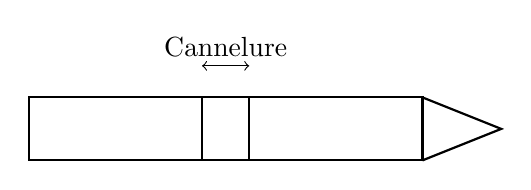
\begin{tikzpicture}[scale=1]

% Projectile
\draw[thick]
(0,0) rectangle (5,0.8);

\draw[thick]
(5,0)
-- (6,0.4)
-- (5,0.8);

% Cannelure
\draw[thick] (2.2,0) -- (2.2,0.8);
\draw[thick] (2.8,0) -- (2.8,0.8);

\draw[<->] (2.2,1.2) -- (2.8,1.2);

\node[above] at (2.5,1.2) {Cannelure};

\end{tikzpicture}

\caption{Exemple de cannelure destinée au sertissage.}
\label{fig:cannelure}

\end{figure}

\section{Influence sur la pression}

Le sertissage augmente généralement la résistance initiale au mouvement du
projectile.

Cette résistance peut modifier :

\begin{itemize}
    \item la montée en pression ;
    \item la combustion de la poudre ;
    \item la vitesse initiale.
\end{itemize}

\section{Influence sur la précision}

L'effet du sertissage sur la précision dépend fortement du contexte.

Selon les armes et les chargements :

\begin{itemize}
    \item il peut améliorer la régularité ;
    \item il peut être sans effet notable ;
    \item il peut parfois dégrader les résultats.
\end{itemize}

L'expérimentation reste souvent nécessaire.

\section{Applications typiques}

Le sertissage est fréquemment utilisé pour :

\begin{itemize}
    \item les revolvers ;
    \item les armes à levier ;
    \item certaines armes semi-automatiques ;
    \item certaines munitions militaires.
\end{itemize}

\section{Le cas du rechargement}

En rechargement, le sertissage doit être appliqué avec discernement.

Un sertissage excessif peut :

\begin{itemize}
    \item déformer le projectile ;
    \item détériorer l'étui ;
    \item nuire à la précision.
\end{itemize}

\section{Quand sertir ?}

Il n'existe pas de règle universelle.

Le besoin dépend notamment :

\begin{itemize}
    \item du type d'arme ;
    \item du projectile ;
    \item du recul ;
    \item du mode d'alimentation ;
    \item de l'usage recherché.
\end{itemize}

\section{Vers les calibres}

Le sertissage constitue l'une des nombreuses caractéristiques pouvant varier
d'une cartouche à l'autre.

Pour comprendre la diversité des munitions existantes, il est maintenant
nécessaire d'aborder la notion de calibre.

\section{À retenir}

\begin{aretenir}

\begin{itemize}
    \item Le sertissage améliore le maintien du projectile.
    \item Il complète la tension de collet.
    \item Le sertissage roulé et le sertissage conique sont les plus répandus.
    \item Un sertissage excessif peut être nuisible.
    \item Son influence dépend fortement de l'application considérée.
\end{itemize}

\end{aretenir}


    \chapter{Le calibre}
    \label{chap:calibre}
    %==============================================================================
% Chapitre 46 - Le calibre
%==============================================================================

\section{Introduction}

Le terme \emph{calibre} est probablement l'un des plus connus dans le domaine
des armes à feu.

Il est pourtant souvent utilisé pour désigner des réalités différentes selon
le contexte.

Le calibre peut en effet faire référence :

\begin{itemize}
    \item au diamètre du projectile ;
    \item au diamètre du canon ;
    \item à une famille de cartouches ;
    \item à une désignation commerciale.
\end{itemize}

Cette diversité d'usages est source de nombreuses confusions.

\begin{aretenir}

Le terme calibre ne possède pas toujours une signification unique.

\end{aretenir}

\section{Définition générale}

Dans son sens le plus courant, le calibre correspond à une dimension
caractéristique liée au diamètre.

Dans les armes à feu, il est généralement exprimé :

\begin{itemize}
    \item en millimètres ;
    \item en fractions de pouce ;
    \item plus rarement sous d'autres formes historiques.
\end{itemize}

\section{Calibre du projectile}

Le calibre peut désigner le diamètre du projectile.

Par exemple :

\begin{itemize}
    \item un projectile de 9 mm possède un diamètre voisin de 9 mm ;
    \item un projectile de .308 pouce possède un diamètre voisin de
          7,82 mm.
\end{itemize}

Cette définition semble simple mais n'est pas toujours suffisante.

\section{Calibre du canon}

Le calibre peut également désigner une dimension du canon.

Or plusieurs méthodes de mesure existent.

Selon les pays et les époques, la mesure peut être réalisée :

\begin{itemize}
    \item entre les sommets des rayures ;
    \item entre les fonds des rayures.
\end{itemize}

Cette différence explique certaines incohérences apparentes.

\section{Les rayures du canon}

Dans un canon rayé, deux diamètres principaux peuvent être définis :

\begin{itemize}
    \item le diamètre entre les sommets des rayures ;
    \item le diamètre entre les fonds des rayures.
\end{itemize}

Le projectile possède généralement un diamètre proche du diamètre à fond de
rayures.



\begin{figure}[htbp]
\centering

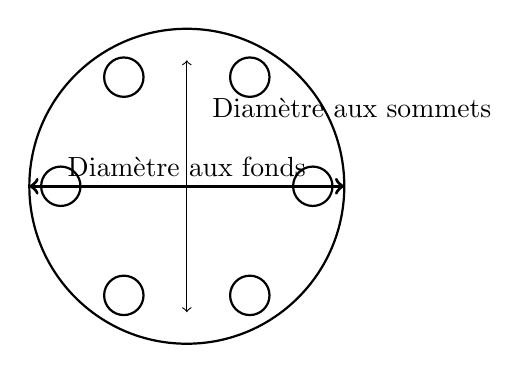
\begin{tikzpicture}[scale=1]

% Fond de rayures
\draw[thick] (0,0) circle (2);

% Sommets
\foreach \a in {0,60,120,180,240,300}
{
    \draw[thick]
    ({1.6*cos(\a)},{1.6*sin(\a)})
    circle (0.25);
}


% Diamètre aux fonds
\draw[<->,very thick]
(-2,0)
--
(2,0);

\node[above]
at (0,0)
{Diamètre aux fonds};

% Diamètre aux sommets
\draw[<->]
(0,-1.6)
--
(0,1.6);

\node[right]
at (0.2,1.0)
{Diamètre aux sommets};

\end{tikzpicture}

\caption{Diamètre aux sommets et diamètre aux fonds des rayures.}
\label{fig:rayures_coupe}

\end{figure}

\section{Exemple du .308 Winchester}

Le .308 Winchester constitue un exemple classique.

Son projectile présente un diamètre nominal de :

\begin{equation}
0,308~\text{pouce}
\end{equation}

soit environ :

\begin{equation}
7,82~\text{mm}
\end{equation}

Pourtant, sa désignation ne fournit aucune information sur la longueur de
l'étui ou les autres caractéristiques de la cartouche.

\section{Millimètres et pouces}

Deux systèmes d'unités coexistent largement :

\begin{itemize}
    \item le système métrique ;
    \item le système impérial.
\end{itemize}

On rencontre ainsi des désignations telles que :

\begin{itemize}
    \item 9 mm ;
    \item 7,62 mm ;
    \item .22 ;
    \item .30 ;
    \item .45.
\end{itemize}

\section{Conversion}

La relation entre pouce et millimètre est :

\begin{equation}
1~\text{pouce}=25,4~\text{mm}
\end{equation}

Cette conversion permet de comparer les différentes désignations.

\section{Des désignations parfois trompeuses}

Certaines appellations historiques ne correspondent pas exactement au
diamètre réel du projectile.

Les raisons sont diverses :

\begin{itemize}
    \item traditions industrielles ;
    \item héritage historique ;
    \item évolutions techniques ;
    \item considérations commerciales.
\end{itemize}

Le calibre indiqué doit donc être considéré comme une désignation plutôt que
comme une mesure exacte.

\section{Familles de calibres}

Plusieurs cartouches peuvent utiliser des projectiles de diamètre voisin.

Par exemple, de nombreuses cartouches utilisent des projectiles de :

\begin{equation}
0,308~\text{pouce}
\end{equation}

tout en présentant des performances très différentes.

\section{Petit calibre et gros calibre}

Les notions de petit et gros calibre dépendent fortement du contexte.

Dans les armes légères, on considère souvent :

\begin{itemize}
    \item les petits calibres ;
    \item les calibres intermédiaires ;
    \item les gros calibres.
\end{itemize}

Ces catégories ne possèdent toutefois pas de limites universelles.

\section{Le cas de l'artillerie}

Dans le domaine de l'artillerie, le calibre désigne généralement le diamètre
intérieur du tube.

On rencontre ainsi :

\begin{itemize}
    \item 105 mm ;
    \item 120 mm ;
    \item 155 mm.
\end{itemize}

\section{Calibre et longueur du tube}

Pour certaines armes, le calibre est également utilisé comme unité de
longueur.

Une pièce d'artillerie peut par exemple être décrite comme :

\begin{quote}
155 mm L/52
\end{quote}

Cela signifie que la longueur du tube vaut 52 fois son calibre.

\begin{figure}[htbp]
\centering

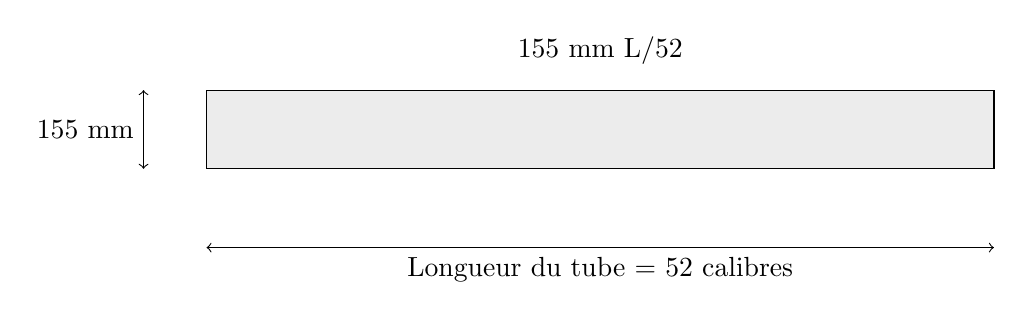
\begin{tikzpicture}[scale=1]

% Tube
\draw[fill=gray!15]
(0,0)
rectangle
(10,1);

% Bouche
\draw[thick]
(10,0)
--
(10,1);

% Calibre
\draw[<->]
(-0.8,0)
--
(-0.8,1);

\node[left]
at (-0.8,0.5)
{155 mm};

% Longueur
\draw[<->]
(0,-1)
--
(10,-1);

\node[below]
at (5,-1)
{Longueur du tube = 52 calibres};

\node[above]
at (5,1.2)
{155 mm L/52};

\end{tikzpicture}

\caption{Exemple de désignation d'une pièce d'artillerie de type 155 mm L/52.}
\label{fig:l52}

\end{figure}

\section{Exemple}

Pour une pièce de :

\begin{equation}
155~\text{mm}
\end{equation}

et :

\begin{equation}
L/52
\end{equation}

la longueur du tube est :

\begin{equation}
155\times52
=
8060~\text{mm}
\end{equation}

soit environ :

\begin{equation}
8,06~\text{m}
\end{equation}

\section{Calibre et performances}

Le calibre influence notamment :

\begin{itemize}
    \item la masse du projectile ;
    \item la quantité d'énergie transportée ;
    \item le recul ;
    \item les effets terminaux.
\end{itemize}

Cependant, le calibre seul ne permet pas de prédire les performances d'une
munition.

\section{Pourquoi le calibre ne suffit pas}

Deux cartouches de même calibre peuvent présenter :

\begin{itemize}
    \item des masses de projectile différentes ;
    \item des vitesses différentes ;
    \item des pressions différentes ;
    \item des énergies très différentes.
\end{itemize}

La désignation complète de la cartouche reste donc indispensable.

\section{Vers les désignations de cartouches}

Le calibre constitue seulement une partie de l'identité d'une munition.

Pour distinguer précisément les nombreuses cartouches existantes, des
systèmes de désignation plus complets ont été développés.

Ils feront l'objet du chapitre suivant.

\section{À retenir}

\begin{aretenir}

\begin{itemize}
    \item Le calibre est généralement lié à une notion de diamètre.
    \item Il peut désigner le projectile, le canon ou une famille de
          cartouches.
    \item Les désignations ne correspondent pas toujours exactement aux
          dimensions réelles.
    \item Deux cartouches de même calibre peuvent avoir des performances très
          différentes.
    \item Le calibre seul ne suffit pas à identifier une munition.
\end{itemize}

\end{aretenir}


    \chapter{Désignation des cartouches}
    \label{chap:designation_cartouches}
    %==============================================================================
% Chapitre 47 - Désignation des cartouches
%==============================================================================

\section{Introduction}

Les cartouches sont désignées selon des conventions qui varient selon les
époques, les pays et les fabricants.

Certaines désignations paraissent intuitives tandis que d'autres semblent
particulièrement énigmatiques.

Comprendre ces appellations permet d'identifier rapidement les principales
caractéristiques d'une munition.

\begin{aretenir}

La désignation d'une cartouche fournit souvent des informations utiles mais
ne décrit pas toujours exactement ses dimensions réelles.

\end{aretenir}

\section{Pourquoi une désignation ?}

Des milliers de cartouches différentes ont été développées au cours de
l'histoire.

Une désignation normalisée permet notamment :

\begin{itemize}
    \item d'identifier une cartouche ;
    \item d'éviter les confusions ;
    \item de garantir la compatibilité des armes ;
    \item de faciliter les échanges techniques.
\end{itemize}

\section{Le système métrique}

De nombreuses cartouches utilisent une désignation de la forme :

\begin{equation}
A \times B
\end{equation}

où :

\begin{itemize}
    \item $A$ représente généralement le calibre nominal ;
    \item $B$ représente généralement la longueur de l'étui.
\end{itemize}

\section{Exemple : 9×19 mm}

La cartouche 9×19 mm possède :

\begin{itemize}
    \item un calibre nominal de 9 mm ;
    \item un étui d'environ 19 mm de longueur.
\end{itemize}

Elle est également connue sous le nom :

\begin{quote}
9 mm Parabellum
\end{quote}

ou :

\begin{quote}
9 mm Luger.
\end{quote}

\section{Exemple : 5,56×45 mm}

La cartouche 5,56×45 mm possède :

\begin{itemize}
    \item un calibre nominal de 5,56 mm ;
    \item un étui d'environ 45 mm.
\end{itemize}

Elle est largement utilisée dans les fusils d'assaut modernes.

\begin{figure}[htbp]
\centering

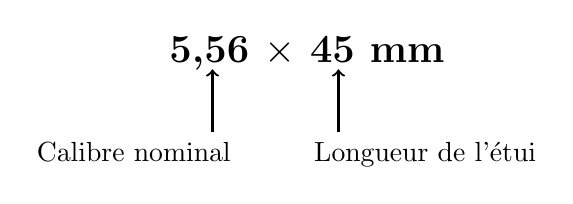
\begin{tikzpicture}[scale=1]

\node[font=\Large\bfseries] (cart) at (0,0)
{5,56 $\times$ 45 mm};

\draw[->,thick]
(-1.2,-1)
--
(-1.2,-0.2);

\node[below]
at (-2.2,-1)
{Calibre nominal};

\draw[->,thick]
(0.4,-1)
--
(0.4,-0.2);

\node[below]
at (1.5,-1)
{Longueur de l'étui};

\end{tikzpicture}

\caption{Exemple de décomposition d'une désignation métrique.}
\label{fig:designation_metrique}

\end{figure}

\section{Exemple : 7,62×51 mm}

La cartouche 7,62×51 mm possède :

\begin{itemize}
    \item un calibre nominal de 7,62 mm ;
    \item un étui d'environ 51 mm.
\end{itemize}

Elle est notamment connue dans sa version civile :

\begin{quote}
.308 Winchester
\end{quote}

bien que les deux cartouches ne soient pas strictement identiques dans tous
les contextes.

\section{Le système impérial}

Dans les pays anglo-saxons, les désignations utilisent souvent le pouce.

On rencontre ainsi :

\begin{itemize}
    \item .22 ;
    \item .30 ;
    \item .308 ;
    \item .357 ;
    \item .45.
\end{itemize}

Le point décimal indique une fraction de pouce.

\section{Exemple : .308 Winchester}

Dans cette désignation :

\begin{itemize}
    \item .308 indique le diamètre nominal du projectile en pouce ;
    \item Winchester désigne l'entreprise ayant développé ou popularisé la
          cartouche.
\end{itemize}

\section{Exemple : .45 ACP}

La désignation ACP signifie :

\begin{quote}
Automatic Colt Pistol
\end{quote}

Le nom fait référence à l'origine historique de la cartouche.

\section{Exemple : .44 Magnum}

Dans certains cas, la désignation comporte un nom commercial.

Le terme Magnum est historiquement associé à des cartouches offrant des
performances supérieures à celles de versions antérieures apparentées.

\section{Exemple : .30-06 Springfield}

Cette désignation est souvent source d'interrogations.

Elle signifie :

\begin{itemize}
    \item .30 : calibre nominal en pouce ;
    \item 06 : année d'adoption 1906 ;
    \item Springfield : référence à l'arsenal associé à son développement.
\end{itemize}

\begin{figure}[htbp]
\centering

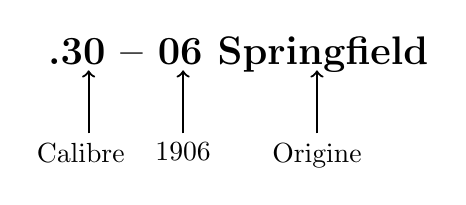
\begin{tikzpicture}[scale=1]

\node[font=\Large\bfseries]
(cart)
at (0,0)
{.30 -- 06 Springfield};

\draw[->,thick]
(-1.9,-1)
--
(-1.9,-0.2);

\node[below]
at (-2,-1)
{Calibre};

\draw[->,thick]
(-0.7,-1)
--
(-0.7,-0.2);

\node[below]
at (-0.7,-1)
{1906};

\draw[->,thick]
(1,-1)
--
(1,-0.2);

\node[below]
at (1,-1)
{Origine};

\end{tikzpicture}

\caption{Exemple de décomposition d'une désignation historique.}
\label{fig:designation_3006}

\end{figure}

\section{Les désignations historiques}

Certaines désignations anciennes reflètent des conventions aujourd'hui
abandonnées.

On peut rencontrer des références liées :

\begin{itemize}
    \item à la masse du projectile ;
    \item à la charge de poudre ;
    \item à l'année d'adoption ;
    \item au fabricant.
\end{itemize}

\section{Le rôle des fabricants}

De nombreux fabricants ont développé leurs propres cartouches.

Le nom du fabricant est souvent conservé dans la désignation :

\begin{itemize}
    \item Winchester ;
    \item Remington ;
    \item Weatherby ;
    \item Norma ;
    \item Lapua.
\end{itemize}

\section{Les désignations militaires}

Les organisations militaires utilisent parfois des désignations spécifiques.

Une même cartouche peut ainsi posséder :

\begin{itemize}
    \item une désignation civile ;
    \item une désignation militaire ;
    \item une référence normalisée.
\end{itemize}

\section{Normalisation}

Afin d'éviter toute ambiguïté, plusieurs organismes définissent des normes.

Ces normes précisent notamment :

\begin{itemize}
    \item les dimensions ;
    \item les tolérances ;
    \item les pressions admissibles ;
    \item les méthodes d'essai.
\end{itemize}

\section{Pourquoi les désignations sont-elles parfois trompeuses ?}

Les appellations historiques ont souvent été conservées malgré les évolutions
techniques.

Par conséquent :

\begin{itemize}
    \item certaines dimensions sont approximatives ;
    \item certaines valeurs sont arrondies ;
    \item certaines désignations ne correspondent plus exactement aux mesures
          réelles.
\end{itemize}

\section{Comment identifier une cartouche ?}

Pour identifier correctement une cartouche, il est souvent nécessaire de
connaître :

\begin{itemize}
    \item son calibre ;
    \item sa longueur d'étui ;
    \item sa désignation complète ;
    \item son éventuelle normalisation.
\end{itemize}

Le calibre seul est rarement suffisant.

\section{Vers les pressions nominales}

Deux cartouches de dimensions voisines peuvent présenter des pressions très
différentes.

L'étude des pressions nominales constitue donc l'étape suivante dans la
compréhension des munitions modernes.

\section{À retenir}

\begin{aretenir}

\begin{itemize}
    \item Les désignations de cartouches suivent plusieurs conventions.
    \item Les systèmes métrique et impérial coexistent.
    \item Certaines désignations reflètent des caractéristiques techniques.
    \item D'autres sont principalement historiques ou commerciales.
    \item Le calibre seul ne permet pas d'identifier précisément une
          cartouche.
\end{itemize}

\end{aretenir}

\begin{figure}[htbp]
\centering

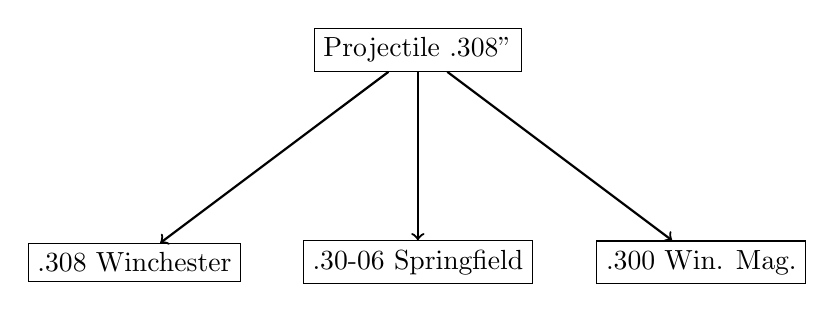
\begin{tikzpicture}[scale=0.9]

% Projectile commun
\node[draw,minimum width=2.5cm]
(P)
at (0,0)
{Projectile .308"};

% Cartouches
\node[draw]
(A)
at (-4,-3)
{.308 Winchester};

\node[draw]
(B)
at (0,-3)
{.30-06 Springfield};

\node[draw]
(C)
at (4,-3)
{.300 Win. Mag.};

\draw[->,thick] (P) -- (A);
\draw[->,thick] (P) -- (B);
\draw[->,thick] (P) -- (C);

\end{tikzpicture}

\caption{Un même diamètre de projectile peut être utilisé dans plusieurs cartouches différentes.}
\label{fig:famille_308}

\end{figure}

\begin{table}[htbp]
\centering
\caption{Exemples de désignations de cartouches.}
\label{tab:designations}

\begin{tabular}{lll}
\hline
Désignation & Système & Signification principale \\
\hline
9×19 mm & Métrique & calibre + longueur d'étui \\
5,56×45 mm & Métrique & calibre + longueur d'étui \\
7,62×51 mm & Métrique & calibre + longueur d'étui \\
.308 Winchester & Impérial & calibre + fabricant \\
.30-06 Springfield & Historique & calibre + année + origine \\
.45 ACP & Impérial & calibre + usage historique \\
\hline
\end{tabular}

\end{table}


    \chapter{Les pressions nominales}
    \label{chap:pressions_nominales}
    %==============================================================================
% Chapitre 48 - Les pressions nominales
%==============================================================================

\section{Introduction}

Lors du tir, la combustion de la poudre produit une grande quantité de gaz.

Ces gaz exercent une pression sur les parois de l'étui, sur la chambre de
l'arme et sur la base du projectile.

Cette pression constitue la source de l'énergie mécanique permettant
l'accélération du projectile.

\begin{aretenir}

La pression est le principal moteur du mouvement du projectile dans le canon.

\end{aretenir}

\section{Qu'est-ce qu'une pression ?}

La pression correspond à une force appliquée sur une surface.

Elle est définie par la relation :

\begin{equation}
P=\frac{F}{S}
\end{equation}

où :

\begin{itemize}
    \item $P$ représente la pression ;
    \item $F$ représente la force ;
    \item $S$ représente la surface.
\end{itemize}

L'unité internationale de pression est le pascal (Pa).

\section{Ordres de grandeur}

Dans la vie courante, les pressions rencontrées sont relativement faibles.

Par exemple :

\begin{itemize}
    \item pression atmosphérique : environ 101 kPa ;
    \item pression d'un pneu automobile : quelques centaines de kPa.
\end{itemize}

Dans une arme à feu, les pressions atteintes sont considérablement plus
élevées.

\section{Pression dans une cartouche}

Lors de la combustion de la poudre :

\begin{itemize}
    \item des gaz sont produits ;
    \item leur température augmente fortement ;
    \item leur volume tend à augmenter ;
    \item la pression s'élève rapidement.
\end{itemize}

Cette augmentation se produit en quelques millisecondes.

\begin{figure}[htbp]
\centering

\begin{tikzpicture}[scale=1]

\draw[->] (0,0) -- (8,0)
node[right] {Temps};

\draw[->] (0,0) -- (0,5)
node[above] {Pression};

\draw[thick]
(0,0)
.. controls (1,4.5) and (2,5) ..
(3,4)
.. controls (5,2.5) and (6.5,1) ..
(8,0.3);

\node at (2.5,4.8)
{$P_{\max}$};

\end{tikzpicture}

\caption{Évolution simplifiée de la pression au cours d'un tir.}
\label{fig:pression_tir}

\end{figure}

\begin{figure}[htbp]
\centering

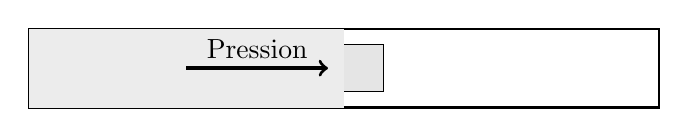
\begin{tikzpicture}[scale=1]

% Canon
\draw[thick] (0,0) rectangle (8,1);

% Projectile
\draw[fill=gray!20]
(4,0.2)
rectangle
(4.5,0.8);

% Gaz
\fill[gray!15]
(0,0)
rectangle
(4,1);

% Force
\draw[->,very thick]
(2,0.5)
--
(3.8,0.5);

\node[above]
at (2.9,0.5)
{Pression};

\end{tikzpicture}

\caption{La pression des gaz exerce une force sur le projectile.}
\label{fig:pression_projectile}

\end{figure}

\section{Pression maximale}

La pression n'est pas constante durant le tir.

Elle augmente rapidement jusqu'à atteindre une valeur maximale.

Cette valeur est souvent appelée :

\begin{quote}
pression maximale admissible
\end{quote}

ou :

\begin{quote}
pression de service maximale.
\end{quote}

\section{Pourquoi limiter la pression ?}

Les armes possèdent des limites mécaniques.

Une pression excessive peut entraîner :

\begin{itemize}
    \item une détérioration de l'arme ;
    \item une rupture de composants ;
    \item des blessures pour le tireur ;
    \item des dommages matériels.
\end{itemize}

La maîtrise de la pression constitue donc un enjeu majeur.

\section{Normalisation}

Les cartouches modernes sont soumises à des normes précises.

Ces normes définissent notamment :

\begin{itemize}
    \item les dimensions ;
    \item les méthodes de mesure ;
    \item les pressions maximales admissibles.
\end{itemize}

Elles garantissent la sécurité et l'interchangeabilité.

\section{La CIP}

En Europe, les pressions sont principalement normalisées par la CIP.

La CIP définit notamment :

\begin{itemize}
    \item les dimensions des chambres ;
    \item les dimensions des cartouches ;
    \item les pressions maximales ;
    \item les procédures d'épreuve.
\end{itemize}

\section{La SAAMI}

Aux États-Unis, un rôle comparable est assuré par la SAAMI.

Cette organisation publie également :

\begin{itemize}
    \item des dimensions ;
    \item des limites de pression ;
    \item des procédures d'essai.
\end{itemize}

\section{Exemples de pressions}

Quelques exemples illustrent les ordres de grandeur rencontrés :

\begin{center}
\begin{tabular}{lc}
\hline
Cartouche & Pression maximale typique \\
\hline
.22 LR & $\approx$ 170 MPa \\
9×19 mm & $\approx$ 235 MPa \\
5,56×45 mm & $\approx$ 430 MPa \\
7,62×51 mm & $\approx$ 415 MPa \\
\hline
\end{tabular}
\end{center}

Les valeurs exactes dépendent des normes utilisées.

\section{Pression et calibre}

Contrairement à une idée répandue, le calibre ne détermine pas à lui seul la
pression.

Deux cartouches de même calibre peuvent fonctionner à des pressions très
différentes.

\section{Pression et vitesse}

Une pression plus élevée permet généralement :

\begin{itemize}
    \item une accélération plus importante ;
    \item une vitesse initiale plus élevée ;
    \item une énergie cinétique plus importante.
\end{itemize}

Cependant, la relation n'est pas strictement proportionnelle.

\section{Pression et longueur de canon}

La pression évolue tout au long du déplacement du projectile.

Elle dépend notamment :

\begin{itemize}
    \item de la combustion de la poudre ;
    \item du volume disponible ;
    \item de la position du projectile.
\end{itemize}

Nous étudierons ces phénomènes en détail dans la partie consacrée à la
balistique intérieure.

\section{Surpression}

On parle de surpression lorsque les limites prévues sont dépassées.

Les causes possibles incluent :

\begin{itemize}
    \item une erreur de chargement ;
    \item une poudre inadaptée ;
    \item un projectile incorrect ;
    \item un enfoncement excessif ;
    \item une obstruction du canon.
\end{itemize}

\section{Sous-pression}

Une pression insuffisante peut également poser problème.

Elle peut provoquer :

\begin{itemize}
    \item un fonctionnement irrégulier ;
    \item une vitesse insuffisante ;
    \item des incidents mécaniques ;
    \item des projectiles bloqués dans le canon.
\end{itemize}

\section{Mesure de la pression}

Les méthodes modernes utilisent généralement :

\begin{itemize}
    \item des capteurs piézoélectriques ;
    \item des équipements instrumentés ;
    \item des bancs d'essai spécialisés.
\end{itemize}

Ces mesures permettent de vérifier la conformité des munitions.

\section{Vers la balistique intérieure}

La pression constitue le phénomène central de la balistique intérieure.

Les chapitres suivants nous permettront de comprendre :

\begin{itemize}
    \item comment elle apparaît ;
    \item comment elle évolue ;
    \item comment elle accélère le projectile.
\end{itemize}

\section{À retenir}

\begin{aretenir}

\begin{itemize}
    \item La pression résulte de la combustion de la poudre.
    \item Elle constitue la source de l'accélération du projectile.
    \item Les pressions sont normalisées par des organismes spécialisés.
    \item Une surpression peut être dangereuse.
    \item La compréhension de la pression est essentielle à la balistique
          intérieure.
\end{itemize}

\end{aretenir}


    \chapter{Classification des munitions}
    \label{chap:classification_munitions}
    %==============================================================================
% Chapitre 49 - Classification des munitions
%==============================================================================

\section{Introduction}

Les munitions existent sous une très grande variété de formes.

Cette diversité résulte des nombreux usages auxquels elles sont destinées :

\begin{itemize}
    \item défense ;
    \item usage militaire ;
    \item chasse ;
    \item tir sportif ;
    \item entraînement ;
    \item applications techniques.
\end{itemize}

Une classification permet de mieux comprendre leurs caractéristiques et leurs
domaines d'emploi.

\begin{aretenir}

Une munition est généralement conçue pour répondre à un besoin précis.

\end{aretenir}

\section{Critères de classification}

Les munitions peuvent être classées selon plusieurs critères :

\begin{itemize}
    \item leur usage ;
    \item leur calibre ;
    \item leur mode de fonctionnement ;
    \item leur projectile ;
    \item leur énergie ;
    \item leur destination.
\end{itemize}

Une même munition peut appartenir simultanément à plusieurs catégories.

\begin{figure}[htbp]
\centering

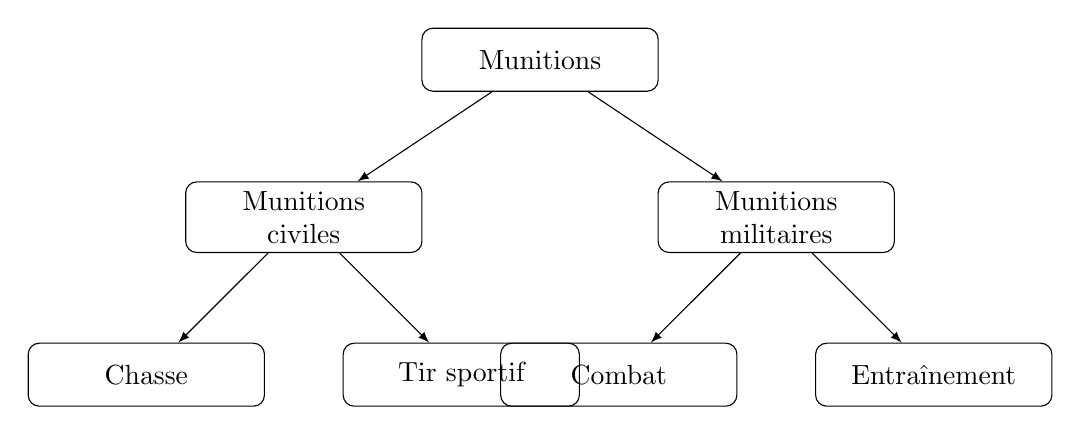
\begin{tikzpicture}[
every node/.style={
draw,
rounded corners,
align=center,
minimum width=3cm,
minimum height=8mm
}
]

\node (M) at (0,0) {Munitions};

\node (C) at (-3,-2) {Munitions\\civiles};
\node (Mil) at (3,-2) {Munitions\\militaires};

\node (Ch) at (-5,-4) {Chasse};
\node (Sp) at (-1,-4) {Tir sportif};

\node (Co) at (1,-4) {Combat};
\node (En) at (5,-4) {Entraînement};

\draw[-latex] (M) -- (C);
\draw[-latex] (M) -- (Mil);

\draw[-latex] (C) -- (Ch);
\draw[-latex] (C) -- (Sp);

\draw[-latex] (Mil) -- (Co);
\draw[-latex] (Mil) -- (En);

\end{tikzpicture}

\caption{Exemple simplifié de classification des munitions.}
\label{fig:classification_munitions}

\end{figure}


\section{Munitions militaires}

Les munitions militaires sont destinées aux forces armées.

Leur conception privilégie généralement :

\begin{itemize}
    \item la fiabilité ;
    \item la robustesse ;
    \item la standardisation ;
    \item la compatibilité logistique.
\end{itemize}

Elles répondent souvent à des spécifications strictes.

\section{Munitions civiles}

Les munitions civiles regroupent de nombreuses catégories :

\begin{itemize}
    \item chasse ;
    \item tir sportif ;
    \item tir récréatif ;
    \item défense.
\end{itemize}

Leurs caractéristiques varient fortement selon l'application.

\section{Munitions de chasse}

Les munitions de chasse sont conçues pour produire des effets adaptés au
gibier recherché.

Le projectile peut être optimisé pour :

\begin{itemize}
    \item l'expansion ;
    \item la pénétration ;
    \item le transfert d'énergie ;
    \item la limitation des ricochets.
\end{itemize}

\section{Munitions de tir sportif}

Le tir sportif privilégie généralement :

\begin{itemize}
    \item la précision ;
    \item la régularité ;
    \item la reproductibilité.
\end{itemize}

Les munitions utilisées sont souvent fabriquées avec des tolérances très
strictes.

\section{Munitions d'entraînement}

Les munitions d'entraînement visent principalement :

\begin{itemize}
    \item la réduction des coûts ;
    \item la sécurité ;
    \item la répétition des exercices.
\end{itemize}

Elles reproduisent souvent le comportement des munitions opérationnelles.

\section{Munitions de défense}

Les munitions de défense sont destinées à l'autoprotection ou aux forces de
l'ordre.

Leurs caractéristiques dépendent du cadre légal et des contraintes
opérationnelles.

\section{Classification selon le projectile}

Une autre méthode consiste à classer les munitions selon leur projectile.

On distingue notamment :

\begin{itemize}
    \item les projectiles blindés ;
    \item les projectiles expansifs ;
    \item les projectiles perforants ;
    \item les projectiles traceurs ;
    \item les projectiles incendiaires.
\end{itemize}

\section{Classification selon l'énergie}

Les munitions peuvent également être regroupées selon leur énergie.

On parle parfois :

\begin{itemize}
    \item de faible puissance ;
    \item de puissance intermédiaire ;
    \item de forte puissance.
\end{itemize}

Ces catégories ne possèdent pas de définition universelle.

\section{Classification selon la vitesse}

Selon leur vitesse initiale, certaines munitions sont qualifiées de :

\begin{itemize}
    \item subsoniques ;
    \item transsoniques ;
    \item supersoniques.
\end{itemize}

Cette distinction influence fortement la balistique extérieure.

\begin{figure}[htbp]
\centering

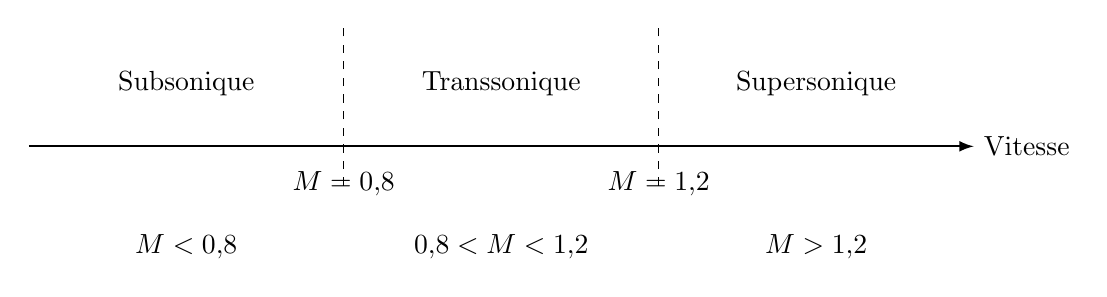
\begin{tikzpicture}[scale=1]

% Axe
\draw[-latex,thick]
(0,0)
--
(12,0)
node[right] {Vitesse};

% Séparations
\draw[dashed]
(4,-0.5)
--
(4,1.5);

\draw[dashed]
(8,-0.5)
--
(8,1.5);

% Zones
\node at (2,0.8)
{Subsonique};

\node at (6,0.8)
{Transsonique};

\node at (10,0.8)
{Supersonique};

% Bornes
\node[below]
at (4,-0.2)
{$M=0{,}8$};

\node[below]
at (8,-0.2)
{$M=1{,}2$};

% Explications
\node[below]
at (2,-1)
{$M<0{,}8$};

\node[below]
at (6,-1)
{$0{,}8<M<1{,}2$};

\node[below]
at (10,-1)
{$M>1{,}2$};

\end{tikzpicture}

\caption{Classification simplifiée selon le nombre de Mach.}
\label{fig:classification_vitesse}

\end{figure}

\section{Classification selon le type d'arme}

Certaines munitions sont conçues pour :

\begin{itemize}
    \item les armes de poing ;
    \item les fusils ;
    \item les carabines ;
    \item les armes automatiques ;
    \item les armes d'artillerie.
\end{itemize}

\section{Munitions à balle et à grenaille}

Dans les armes lisses, on distingue généralement :

\begin{itemize}
    \item les cartouches à balle unique ;
    \item les cartouches à grenaille.
\end{itemize}

Leur comportement balistique est très différent.

\section{Munitions spéciales}

Certaines munitions répondent à des besoins particuliers :

\begin{itemize}
    \item traçantes ;
    \item perforantes ;
    \item incendiaires ;
    \item d'exercice ;
    \item à blanc.
\end{itemize}

Leurs caractéristiques seront détaillées dans des chapitres ultérieurs.

\section{Pourquoi autant de variantes ?}

Chaque usage impose des contraintes différentes.

Une munition idéale pour le tir de précision n'est pas nécessairement adaptée :

\begin{itemize}
    \item à la chasse ;
    \item à l'entraînement ;
    \item à un usage militaire.
\end{itemize}

Cette diversité explique le grand nombre de cartouches existantes.

\section{Vers les munitions militaires}

Parmi toutes les catégories étudiées, les munitions militaires occupent une
place particulière en raison de leur influence historique sur le développement
de nombreuses cartouches modernes.

Le chapitre suivant leur sera consacré.

\section{À retenir}

\begin{aretenir}

\begin{itemize}
    \item Les munitions peuvent être classées selon de nombreux critères.
    \item Une même cartouche peut appartenir à plusieurs catégories.
    \item L'usage recherché influence fortement la conception.
    \item Les projectiles constituent un critère de classification majeur.
    \item La diversité des munitions reflète la diversité des besoins.
\end{itemize}

\end{aretenir}


    \chapter{Les munitions militaires}
    \label{chap:munitions_militaires}
    %==============================================================================
% Chapitre 50 - Les munitions militaires
%==============================================================================

\section{Introduction}

Depuis l'apparition des armes à feu modernes, les besoins militaires ont
fortement influencé le développement des munitions.

Les conflits armés ont conduit à la création de nombreuses cartouches devenues
par la suite des références dans le domaine civil.

Aujourd'hui encore, les exigences militaires constituent un moteur important
de l'innovation balistique.

\begin{aretenir}

De nombreuses cartouches civiles modernes trouvent leur origine dans des
munitions développées pour un usage militaire.

\end{aretenir}

\section{Objectifs militaires}

Une munition militaire doit répondre à plusieurs exigences parfois
contradictoires :

\begin{itemize}
    \item efficacité ;
    \item fiabilité ;
    \item robustesse ;
    \item coût maîtrisé ;
    \item facilité de production ;
    \item compatibilité logistique.
\end{itemize}

Ces contraintes influencent fortement sa conception.

\section{Standardisation}

Les armées utilisent généralement des munitions standardisées.

Cette standardisation facilite :

\begin{itemize}
    \item la fabrication ;
    \item le stockage ;
    \item le transport ;
    \item l'interopérabilité entre unités.
\end{itemize}

Elle constitue un élément essentiel de la logistique militaire.

\section{Le rôle de l'OTAN}

Au sein de l'OTAN, plusieurs cartouches ont été normalisées afin de permettre
leur emploi par différents pays.

Parmi les plus connues figurent :

\begin{itemize}
    \item le 5,56×45 mm ;
    \item le 7,62×51 mm ;
    \item le 9×19 mm.
\end{itemize}

Ces munitions sont utilisées par de nombreuses forces armées.

\section{La fiabilité avant tout}

Une munition militaire doit fonctionner dans des conditions difficiles :

\begin{itemize}
    \item températures extrêmes ;
    \item humidité ;
    \item poussière ;
    \item vibrations ;
    \item stockage prolongé.
\end{itemize}

La fiabilité constitue souvent le critère prioritaire.

\section{Production à grande échelle}

Les besoins militaires peuvent atteindre plusieurs millions de cartouches.

Les procédés industriels doivent donc permettre :

\begin{itemize}
    \item une cadence élevée ;
    \item une qualité constante ;
    \item un coût raisonnable.
\end{itemize}

\section{Munitions d'arme de poing}

Les armes de poing militaires utilisent généralement des cartouches offrant :

\begin{itemize}
    \item un recul modéré ;
    \item une bonne fiabilité ;
    \item un encombrement réduit.
\end{itemize}

Le 9×19 mm constitue aujourd'hui l'exemple le plus répandu.

\section{Munitions de fusil}

Les fusils militaires utilisent des cartouches adaptées aux engagements à
moyenne distance.

Leurs caractéristiques doivent permettre :

\begin{itemize}
    \item une portée suffisante ;
    \item une trajectoire acceptable ;
    \item une masse raisonnable.
\end{itemize}

\section{Évolution historique}

Durant le XX\ieme\ siècle, plusieurs tendances majeures sont apparues :

\begin{itemize}
    \item réduction du calibre ;
    \item augmentation de la vitesse ;
    \item allègement de la munition ;
    \item amélioration de la portée utile.
\end{itemize}

\begin{figure}[htbp]
\centering

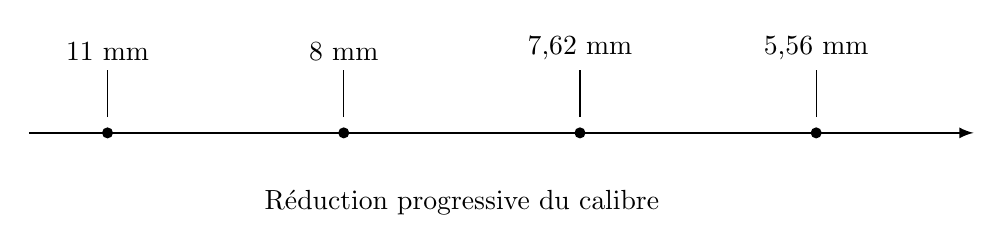
\begin{tikzpicture}[scale=1]

% Ligne principale
\draw[-latex,thick] (0,0) -- (12,0);

% Jalons
\foreach \x/\txt in {
1/{11 mm},
4/{8 mm},
7/{7,62 mm},
10/{5,56 mm}
}
{
    \fill (\x,0) circle (2pt);
    \draw (\x,0.2) -- (\x,0.8);
    \node[above] at (\x,0.8) {\txt};
}

\node[below] at (5.5,-0.6)
{Réduction progressive du calibre};

\end{tikzpicture}

\caption{Évolution simplifiée de certains calibres militaires au cours du temps.}
\label{fig:evolution_calibres_militaires}

\end{figure}

\section{Du calibre intermédiaire}

Après la Seconde Guerre mondiale, plusieurs armées ont adopté le concept de
cartouche intermédiaire.

Cette approche vise à trouver un compromis entre :

\begin{itemize}
    \item puissance ;
    \item portée ;
    \item contrôle du recul ;
    \item quantité de munitions transportées.
\end{itemize}

\begin{figure}[htbp]
\centering

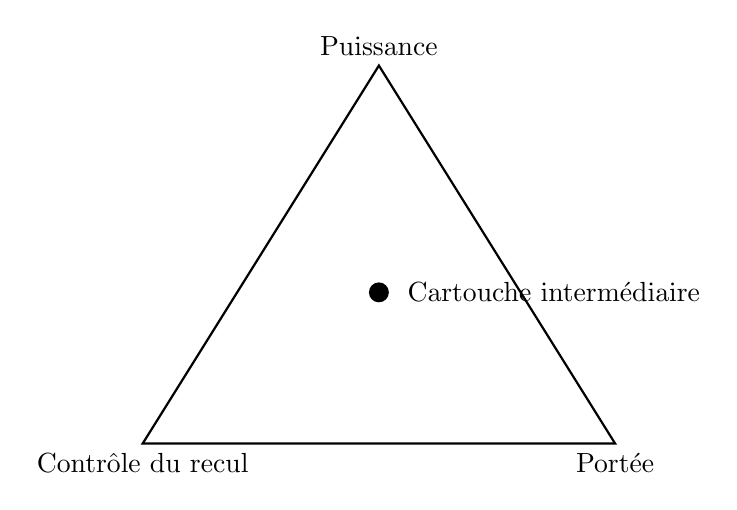
\begin{tikzpicture}[scale=1.2]

% Triangle
\draw[thick]
(0,0)
--
(5,0)
--
(2.5,4)
--
cycle;

% Sommets
\node[below] at (0,0)
{Contrôle du recul};

\node[below] at (5,0)
{Portée};

\node[above] at (2.5,4)
{Puissance};

% Point central
\fill (2.5,1.6) circle (3pt);

\node[right] at (2.7,1.6)
{Cartouche intermédiaire};

\end{tikzpicture}

\caption{Le calibre intermédiaire constitue un compromis entre plusieurs exigences contradictoires.}
\label{fig:calibre_intermediaire}

\end{figure}

\section{Exemple du 5,56×45 mm}

Le 5,56×45 mm est conçu pour offrir :

\begin{itemize}
    \item une vitesse élevée ;
    \item une masse réduite ;
    \item un recul limité ;
    \item une bonne capacité d'emport.
\end{itemize}

Son adoption a profondément influencé les armes militaires modernes.

\section{Exemple du 7,62×51 mm}

Le 7,62×51 mm conserve :

\begin{itemize}
    \item une énergie importante ;
    \item une portée significative ;
    \item une bonne capacité de pénétration.
\end{itemize}

Il reste largement utilisé dans certaines fonctions spécialisées.

\section{Munitions de mitrailleuse}

Les mitrailleuses utilisent souvent les mêmes cartouches que les fusils ou des
versions plus puissantes.

Les contraintes principales concernent :

\begin{itemize}
    \item l'échauffement ;
    \item la cadence de tir ;
    \item l'alimentation continue.
\end{itemize}

\section{Les munitions traçantes}

Les projectiles traçants produisent une trace lumineuse visible pendant le vol.

Ils permettent notamment :

\begin{itemize}
    \item l'observation de la trajectoire ;
    \item le réglage du tir ;
    \item la désignation d'objectif.
\end{itemize}

\section{Les munitions perforantes}

Certaines munitions sont conçues pour améliorer la pénétration.

Elles utilisent souvent un noyau réalisé dans un matériau plus dur que le
plomb.

\section{Les munitions incendiaires}

Les munitions incendiaires embarquent une composition capable de produire un
effet thermique important après impact.

\section{Les munitions d'exercice}

Les forces armées utilisent également :

\begin{itemize}
    \item des munitions d'entraînement ;
    \item des munitions à blanc ;
    \item des cartouches d'exercice inertes.
\end{itemize}

Ces munitions réduisent les coûts et améliorent la sécurité.

\begin{figure}[htbp]
\centering

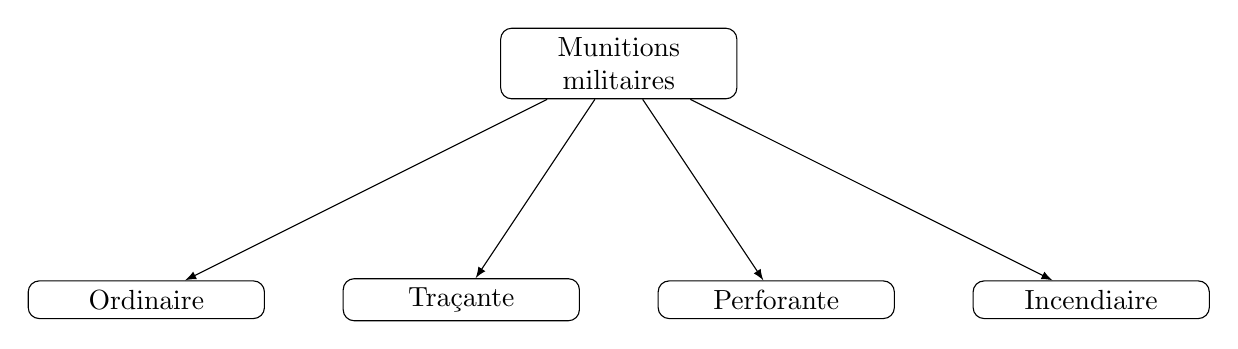
\begin{tikzpicture}[
every node/.style={
draw,
rounded corners,
align=center,
minimum width=3cm
}
]

\node (M) at (0,0) {Munitions\\militaires};

\node (B) at (-6,-3) {Ordinaire};
\node (T) at (-2,-3) {Traçante};
\node (P) at (2,-3) {Perforante};
\node (I) at (6,-3) {Incendiaire};

\draw[-latex] (M) -- (B);
\draw[-latex] (M) -- (T);
\draw[-latex] (M) -- (P);
\draw[-latex] (M) -- (I);

\end{tikzpicture}

\caption{Exemples de familles de munitions militaires spécialisées.}
\label{fig:types_munitions_militaires}

\end{figure}

\section{Stockage militaire}

Le stockage constitue un aspect essentiel de la logistique.

Les munitions doivent conserver leurs performances pendant de nombreuses
années.

Des procédures strictes encadrent :

\begin{itemize}
    \item le transport ;
    \item le stockage ;
    \item la surveillance des lots.
\end{itemize}

\section{Vers les projectiles militaires}

Les contraintes militaires ont conduit au développement de nombreux types de
projectiles spécialisés.

Le chapitre suivant examinera plus en détail les différentes catégories de
projectiles employés dans les munitions militaires.

\section{À retenir}

\begin{aretenir}

\begin{itemize}
    \item Les besoins militaires ont fortement influencé l'évolution des
          munitions modernes.
    \item La fiabilité et la standardisation constituent des objectifs majeurs.
    \item Les cartouches militaires doivent répondre à des contraintes
          logistiques importantes.
    \item De nombreuses variantes spécialisées existent.
    \item Les munitions militaires ont inspiré de nombreuses cartouches
          civiles.
\end{itemize}

\end{aretenir}


    \chapter{Les projectiles militaires}
    \label{chap:projectiles_militaires}
    %==============================================================================
% Chapitre 51 - Les projectiles militaires
%==============================================================================

\section{Introduction}

Les besoins militaires ont conduit au développement d'un grand nombre de
projectiles spécialisés.

Bien que leur apparence extérieure soit souvent similaire, leur construction
interne peut varier considérablement selon l'effet recherché.

\begin{aretenir}

La forme extérieure d'un projectile ne permet pas toujours de déterminer sa
fonction.

\end{aretenir}

\section{Projectile ordinaire}

Le projectile ordinaire constitue la forme la plus répandue.

Il est généralement composé :

\begin{itemize}
    \item d'un noyau dense ;
    \item d'une chemise métallique ;
    \item parfois d'une base spécifique.
\end{itemize}

Il constitue souvent la référence à partir de laquelle sont développées les
autres variantes.

\section{Projectile blindé}

Le projectile blindé est généralement désigné par l'acronyme :

\begin{quote}
FMJ --- Full Metal Jacket
\end{quote}

Il possède une chemise métallique recouvrant la majeure partie du noyau.

Cette conception améliore notamment :

\begin{itemize}
    \item la résistance mécanique ;
    \item l'alimentation dans les armes automatiques ;
    \item la régularité de fabrication.
\end{itemize}

\begin{figure}[htbp]
\centering

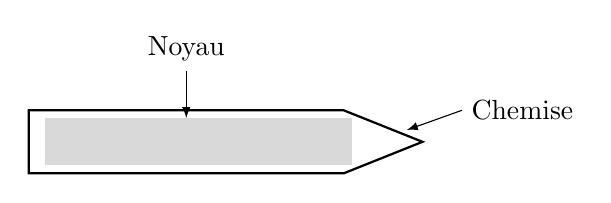
\begin{tikzpicture}[scale=1]

% Contour extérieur
\draw[thick]
(0,0)
-- (0,0.8)
-- (4,0.8)
-- (5,0.4)
-- (4,0)
-- cycle;

% Noyau
\fill[gray!30]
(0.2,0.1)
rectangle
(4.1,0.7);

% Légendes
\draw[-latex]
(2,1.3)
--
(2,0.7);

\node[above]
at (2,1.3)
{Noyau};

\draw[-latex]
(5.5,0.8)
--
(4.8,0.55);

\node[right]
at (5.5,0.8)
{Chemise};

\end{tikzpicture}

\caption{Structure simplifiée d'un projectile blindé (FMJ).}
\label{fig:fmj}

\end{figure}

\section{Contraintes des conventions internationales}

Certaines conventions internationales influencent la conception des
projectiles militaires.

Ces contraintes ont notamment favorisé l'emploi de projectiles blindés dans
de nombreuses armées.

\section{Projectile perforant}

Le projectile perforant est conçu pour améliorer la pénétration des matériaux
résistants.

Pour cela, il utilise généralement :

\begin{itemize}
    \item un noyau plus dur ;
    \item une géométrie adaptée ;
    \item une masse concentrée.
\end{itemize}

\begin{figure}[htbp]
\centering

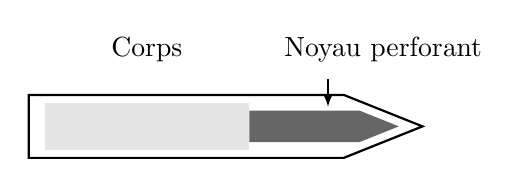
\begin{tikzpicture}[scale=1]

% Chemise
\draw[thick]
(0,0)
-- (0,0.8)
-- (4,0.8)
-- (5,0.4)
-- (4,0)
-- cycle;

% Noyau classique
\fill[gray!20]
(0.2,0.1)
rectangle
(2.8,0.7);

% Noyau perforant
\fill[black!60]
(2.8,0.2)
--
(4.2,0.2)
--
(4.7,0.4)
--
(4.2,0.6)
--
(2.8,0.6)
--
cycle;

\node[above]
at (1.5,1.1)
{Corps};

\node[above]
at (4.5,1.1)
{Noyau perforant};

\draw[-latex]
(3.8,1.0)
--
(3.8,0.65);

\end{tikzpicture}

\caption{Exemple simplifié de projectile perforant.}
\label{fig:perforant}

\end{figure}

\section{Noyaux perforants}

Les noyaux perforants peuvent être réalisés dans différents matériaux.

Les caractéristiques recherchées sont notamment :

\begin{itemize}
    \item une dureté élevée ;
    \item une bonne résistance mécanique ;
    \item une géométrie stable à l'impact.
\end{itemize}

\section{Projectile traceur}

Le projectile traceur contient une composition pyrotechnique située
généralement dans sa partie arrière.

Pendant le vol, cette composition produit une trace lumineuse visible.

\begin{figure}[htbp]
\centering

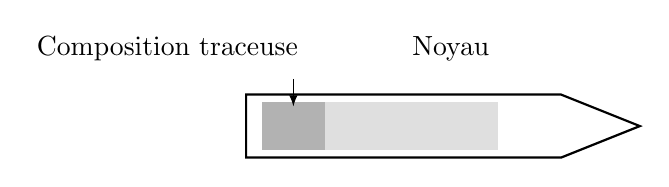
\begin{tikzpicture}[scale=1]

% Chemise
\draw[thick]
(0,0)
-- (0,0.8)
-- (4,0.8)
-- (5,0.4)
-- (4,0)
-- cycle;

% Noyau
\fill[gray!25]
(0.2,0.1)
rectangle
(3.2,0.7);

% Traceur
\fill[gray!60]
(0.2,0.1)
rectangle
(1.0,0.7);

% Légendes
\node[above]
at (2.6,1.1)
{Noyau};

\node[above]
at (-1,1.1)
{Composition traceuse};

\draw[-latex]
(0.6,1.0)
--
(0.6,0.65);

\end{tikzpicture}

\caption{Structure simplifiée d'un projectile traceur.}
\label{fig:traceur}

\end{figure}

\section{Intérêt des traceurs}

Les projectiles traceurs permettent :

\begin{itemize}
    \item de visualiser la trajectoire ;
    \item de corriger le tir ;
    \item de désigner une cible ;
    \item de faciliter certaines coordinations tactiques.
\end{itemize}

\section{Limites des traceurs}

L'utilisation de traceurs présente également certains inconvénients :

\begin{itemize}
    \item révélation de la position du tireur ;
    \item visibilité accrue du tir ;
    \item comportement balistique parfois légèrement différent.
\end{itemize}

\section{Projectile incendiaire}

Les projectiles incendiaires contiennent une composition destinée à produire
un effet thermique important après impact.

Ils sont principalement employés contre certains matériels.

\section{Projectile perforant-incendiaire}

Certaines conceptions combinent plusieurs fonctions.

Un projectile peut ainsi être à la fois :

\begin{itemize}
    \item perforant ;
    \item incendiaire.
\end{itemize}

Cette combinaison vise à améliorer l'efficacité contre certains objectifs.

\begin{figure}[htbp]
\centering

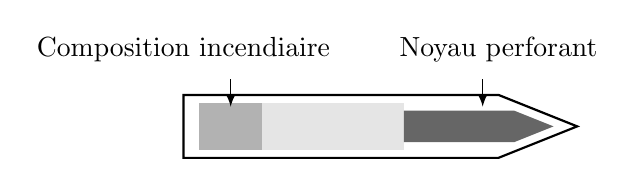
\begin{tikzpicture}[scale=1]

% Chemise
\draw[thick]
(0,0)
-- (0,0.8)
-- (4,0.8)
-- (5,0.4)
-- (4,0)
-- cycle;

% Composition incendiaire
\fill[gray!60]
(0.2,0.1)
rectangle
(1.0,0.7);

% Corps
\fill[gray!20]
(1.0,0.1)
rectangle
(2.8,0.7);

% Noyau perforant
\fill[black!60]
(2.8,0.2)
--
(4.2,0.2)
--
(4.7,0.4)
--
(4.2,0.6)
--
(2.8,0.6)
--
cycle;

\node[above]
at (0,1.1)
{Composition incendiaire};

\node[above]
at (4,1.1)
{Noyau perforant};

\draw[-latex]
(0.6,1.0)
--
(0.6,0.65);

\draw[-latex]
(3.8,1.0)
--
(3.8,0.65);

\end{tikzpicture}

\caption{Exemple simplifié de projectile perforant-incendiaire.}
\label{fig:perforant_incendiaire}

\end{figure}

\section{Projectile explosif}

Les projectiles explosifs de petit calibre restent relativement rares.

Ils sont davantage rencontrés dans les munitions de moyen et gros calibre.

\section{Projectile d'exercice}

Les armées utilisent également des projectiles destinés à l'instruction.

Leur objectif principal est de reproduire certaines caractéristiques des
munitions opérationnelles tout en réduisant les coûts.

\section{Projectile à blanc}

Les cartouches à blanc ne comportent généralement pas de projectile.

Elles permettent :

\begin{itemize}
    \item l'entraînement ;
    \item certaines cérémonies ;
    \item des simulations tactiques.
\end{itemize}

\section{Identification visuelle}

De nombreuses munitions militaires utilisent des marquages spécifiques.

Ceux-ci peuvent prendre différentes formes :

\begin{itemize}
    \item couleurs ;
    \item vernis ;
    \item marquages de pointe ;
    \item inscriptions.
\end{itemize}

\section{Normalisation}

Les systèmes d'identification varient selon :

\begin{itemize}
    \item les pays ;
    \item les époques ;
    \item les fabricants.
\end{itemize}

Aucune règle universelle ne s'applique à l'ensemble des munitions militaires.

\section{Effets recherchés}

Selon leur conception, les projectiles militaires peuvent privilégier :

\begin{itemize}
    \item la pénétration ;
    \item la visibilité ;
    \item l'effet thermique ;
    \item la précision ;
    \item la polyvalence.
\end{itemize}

\section{Vers les munitions spéciales}

Les projectiles militaires ne représentent qu'une partie de la diversité des
munitions modernes.

Le chapitre suivant abordera d'autres catégories de munitions spécialisées.

\section{À retenir}

\begin{aretenir}

\begin{itemize}
    \item Les projectiles militaires existent sous de nombreuses variantes.
    \item Les projectiles blindés sont les plus répandus.
    \item Les projectiles perforants améliorent la pénétration.
    \item Les traceurs permettent d'observer la trajectoire.
    \item Certaines conceptions combinent plusieurs fonctions.
\end{itemize}

\end{aretenir}


    \chapter{Les munitions spéciales}
    \label{chap:munitions_speciales}
    %==============================================================================
% Chapitre 52 - Les munitions spéciales
%==============================================================================

\section{Introduction}

Toutes les munitions ne sont pas destinées à produire un simple effet de
perforation ou de neutralisation.

Au fil du temps, de nombreuses munitions spécialisées ont été développées afin
de répondre à des besoins particuliers.

Ces munitions peuvent être destinées :

\begin{itemize}
    \item à l'entraînement ;
    \item au réglage du tir ;
    \item à la signalisation ;
    \item à la simulation ;
    \item à certaines applications techniques.
\end{itemize}

\begin{aretenir}

Une munition spéciale est conçue pour remplir une fonction particulière qui
dépasse le simple tir conventionnel.

\end{aretenir}

\section{Diversité des munitions spéciales}

Les munitions spéciales regroupent une famille très vaste.

On y trouve notamment :

\begin{itemize}
    \item les cartouches à blanc ;
    \item les cartouches d'exercice ;
    \item les munitions traçantes ;
    \item les munitions de signalisation ;
    \item les munitions de réglage ;
    \item les munitions non létales.
\end{itemize}

\begin{figure}[htbp]
\centering

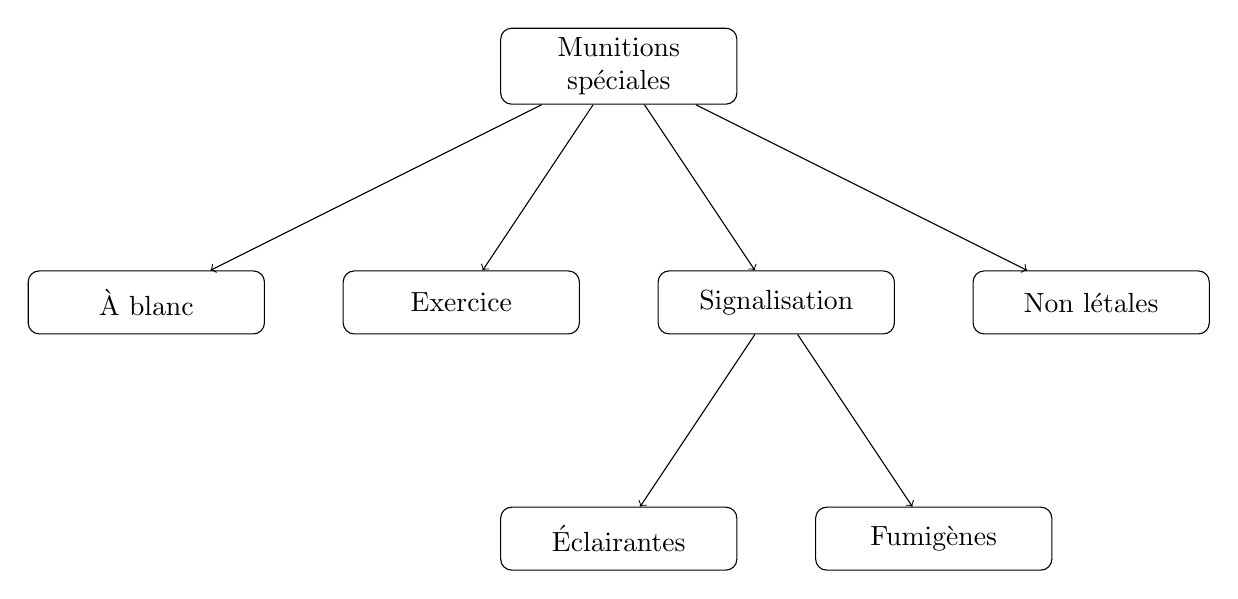
\begin{tikzpicture}[
every node/.style={
draw,
rounded corners,
align=center,
minimum width=3cm,
minimum height=8mm
}
]

\node (M) at (0,0) {Munitions\\spéciales};

\node (B) at (-6,-3) {À blanc};
\node (E) at (-2,-3) {Exercice};
\node (S) at (2,-3) {Signalisation};
\node (N) at (6,-3) {Non létales};

\draw[->] (M) -- (B);
\draw[->] (M) -- (E);
\draw[->] (M) -- (S);
\draw[->] (M) -- (N);

\node (Ec) at (0,-6) {Éclairantes};
\node (Fu) at (4,-6) {Fumigènes};

\draw[->] (S) -- (Ec);
\draw[->] (S) -- (Fu);

\end{tikzpicture}

\caption{Exemple simplifié de classification des munitions spéciales.}
\label{fig:munitions_speciales}

\end{figure}

\section{Cartouches à blanc}

Les cartouches à blanc ne propulsent généralement pas de projectile.

Elles produisent néanmoins :

\begin{itemize}
    \item du bruit ;
    \item une flamme de bouche ;
    \item des gaz sous pression.
\end{itemize}

Elles sont largement utilisées pour l'instruction et les cérémonies.

\begin{figure}[htbp]
\centering

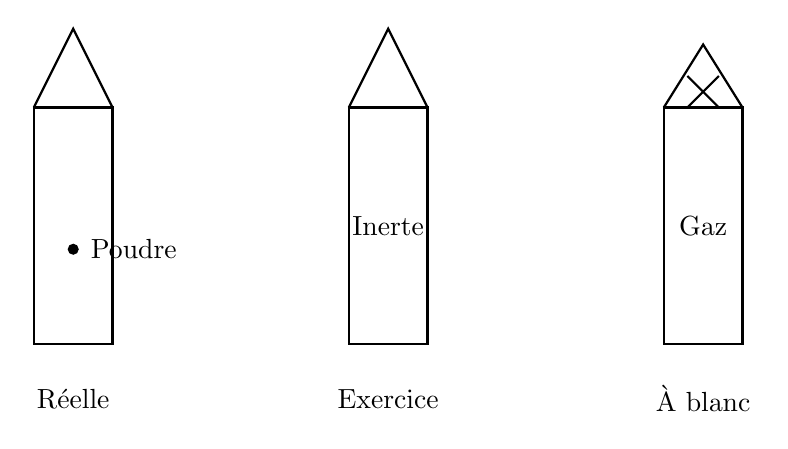
\begin{tikzpicture}[scale=1]

% Réelle
\begin{scope}

\draw[thick] (0,0) rectangle (1,3);
\draw[thick] (0,3) -- (0.5,4) -- (1,3);

\node at (0.5,-0.7) {Réelle};

\fill (0.5,1.2) circle (2pt);
\node[right] at (0.6,1.2) {Poudre};

\end{scope}

% Exercice
\begin{scope}[xshift=4cm]

\draw[thick] (0,0) rectangle (1,3);
\draw[thick] (0,3) -- (0.5,4) -- (1,3);

\node at (0.5,-0.7) {Exercice};

\node at (0.5,1.5) {Inerte};

\end{scope}

% Blanc
\begin{scope}[xshift=8cm]

\draw[thick] (0,0) rectangle (1,3);

\draw[thick]
(0,3)
--
(0.5,3.8)
--
(1,3);

\draw[thick]
(0.3,3.4)
--
(0.7,3.0);

\draw[thick]
(0.3,3.0)
--
(0.7,3.4);

\node at (0.5,-0.7) {À blanc};

\node at (0.5,1.5) {Gaz};

\end{scope}

\end{tikzpicture}

\caption{Comparaison simplifiée entre une cartouche réelle, une cartouche d'exercice et une cartouche à blanc.}
\label{fig:types_cartouches}

\end{figure}

\section{Risques associés}

L'absence de projectile ne signifie pas l'absence de danger.

Les gaz expulsés à la bouche peuvent provoquer des blessures à courte
distance.

Des règles de sécurité spécifiques doivent être appliquées.

\section{Cartouches d'exercice}

Les cartouches d'exercice reproduisent généralement :

\begin{itemize}
    \item les dimensions ;
    \item la masse ;
    \item l'encombrement ;
    \item le fonctionnement mécanique.
\end{itemize}

Elles permettent l'entraînement sans tir réel.

\section{Cartouches inertes}

Certaines cartouches sont totalement inertes.

Elles ne contiennent :

\begin{itemize}
    \item ni amorce active ;
    \item ni poudre ;
    \item ni composition pyrotechnique.
\end{itemize}

Elles servent principalement à l'instruction.

\section{Munitions de signalisation}

Certaines munitions sont destinées à transmettre une information visuelle.

Elles peuvent produire :

\begin{itemize}
    \item une lumière ;
    \item une couleur ;
    \item un signal visible à grande distance.
\end{itemize}

\section{Munitions éclairantes}

Les munitions éclairantes sont conçues pour illuminer temporairement une zone.

Elles sont utilisées :

\begin{itemize}
    \item pour l'observation ;
    \item pour la surveillance ;
    \item pour certaines opérations nocturnes.
\end{itemize}

\section{Munitions fumigènes}

Les munitions fumigènes produisent un nuage de fumée.

Celui-ci peut servir :

\begin{itemize}
    \item au marquage ;
    \item à la signalisation ;
    \item au camouflage.
\end{itemize}

\section{Munitions de réglage}

Certaines munitions permettent d'observer plus facilement l'impact ou la
trajectoire.

Elles facilitent :

\begin{itemize}
    \item le réglage des armes ;
    \item le contrôle des tirs ;
    \item l'entraînement.
\end{itemize}

\section{Munitions non létales}

Certaines applications nécessitent de limiter les effets produits.

Les munitions dites non létales cherchent à réduire le risque de blessures
graves tout en conservant un effet incapacitant.

\section{Limites du terme non létal}

L'expression \emph{non létal} peut être trompeuse.

Toute munition capable de transmettre une quantité suffisante d'énergie peut
présenter un danger.

C'est pourquoi l'expression :

\begin{quote}
à létalité réduite
\end{quote}

est parfois préférée.

\section{Applications policières}

Les forces de l'ordre utilisent diverses munitions spécialisées.

Leur objectif peut être :

\begin{itemize}
    \item le maintien de l'ordre ;
    \item la neutralisation temporaire ;
    \item la dispersion ;
    \item l'interpellation.
\end{itemize}

\section{Applications industrielles}

Certaines munitions sont utilisées en dehors du domaine militaire ou sportif.

On peut citer notamment :

\begin{itemize}
    \item les outils de scellement ;
    \item certaines applications pyrotechniques ;
    \item certains dispositifs de sécurité.
\end{itemize}

\section{Contraintes réglementaires}

Les munitions spéciales sont souvent soumises à des réglementations
particulières.

Ces règles varient selon :

\begin{itemize}
    \item les pays ;
    \item les usages ;
    \item les catégories de munitions.
\end{itemize}

\section{Pourquoi autant de variantes ?}

Chaque mission impose des contraintes spécifiques.

Une munition optimisée pour l'éclairage ne peut pas remplir efficacement une
fonction de signalisation ou d'entraînement.

Cette spécialisation explique la grande diversité observée.

\begin{figure}[htbp]
\centering

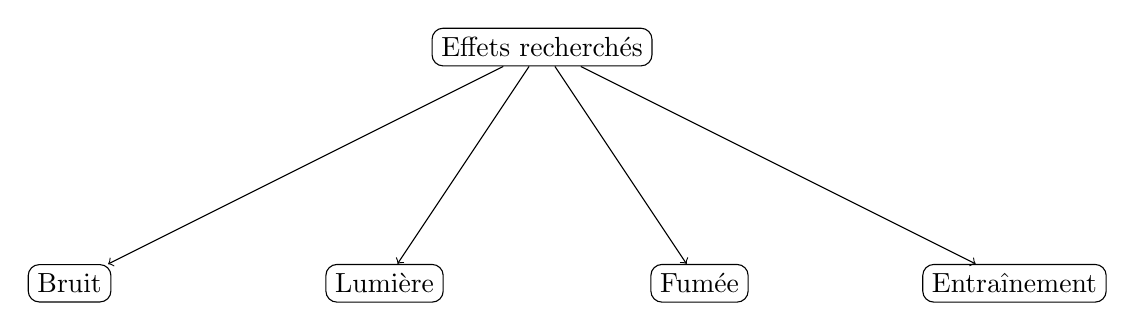
\begin{tikzpicture}[scale=1]

\node[draw,rounded corners]
(M)
at (0,0)
{Effets recherchés};

\node[draw,rounded corners]
(B)
at (-6,-3)
{Bruit};

\node[draw,rounded corners]
(L)
at (-2,-3)
{Lumière};

\node[draw,rounded corners]
(F)
at (2,-3)
{Fumée};

\node[draw,rounded corners]
(E)
at (6,-3)
{Entraînement};

\draw[->] (M) -- (B);
\draw[->] (M) -- (L);
\draw[->] (M) -- (F);
\draw[->] (M) -- (E);

\end{tikzpicture}

\caption{Exemples d'effets recherchés avec les munitions spéciales.}
\label{fig:effets_munitions_speciales}

\end{figure}

\section{Vers les munitions de chasse}

Les munitions spéciales illustrent la capacité d'adaptation des technologies
balistiques.

Nous allons maintenant revenir à un domaine majeur du monde civil : les
munitions de chasse.

\section{À retenir}

\begin{aretenir}

\begin{itemize}
    \item Les munitions spéciales répondent à des besoins particuliers.
    \item Les cartouches à blanc et les cartouches d'exercice sont largement
          utilisées pour l'instruction.
    \item Les munitions de signalisation remplissent des fonctions
          d'information et de repérage.
    \item Les munitions non létales restent potentiellement dangereuses.
    \item La spécialisation des usages explique la grande diversité des
          conceptions.
\end{itemize}

\end{aretenir}


    \chapter{Les munitions de chasse}
    \label{chap:munitions_chasse}
    %==============================================================================
% Chapitre 53 - Les munitions de chasse
%==============================================================================

\section{Introduction}

La chasse constitue l'une des principales applications civiles des armes à feu.

Au fil du temps, de nombreuses munitions ont été développées afin de répondre
à des besoins très différents selon le type de gibier recherché.

Les contraintes rencontrées diffèrent souvent de celles du domaine militaire.

\begin{aretenir}

Une munition de chasse doit permettre un prélèvement efficace tout en limitant
autant que possible les souffrances de l'animal.

\end{aretenir}

\section{Diversité des situations}

Les conditions de chasse peuvent varier considérablement.

Les paramètres à prendre en compte incluent notamment :

\begin{itemize}
    \item la taille du gibier ;
    \item la distance de tir ;
    \item l'environnement ;
    \item le type d'arme utilisée.
\end{itemize}

Cette diversité explique l'existence d'un grand nombre de munitions.

\section{Petit gibier et grand gibier}

On distingue généralement :

\begin{itemize}
    \item le petit gibier ;
    \item le grand gibier.
\end{itemize}

Les caractéristiques recherchées pour les munitions diffèrent fortement entre
ces deux catégories.

\begin{figure}[htbp]
\centering

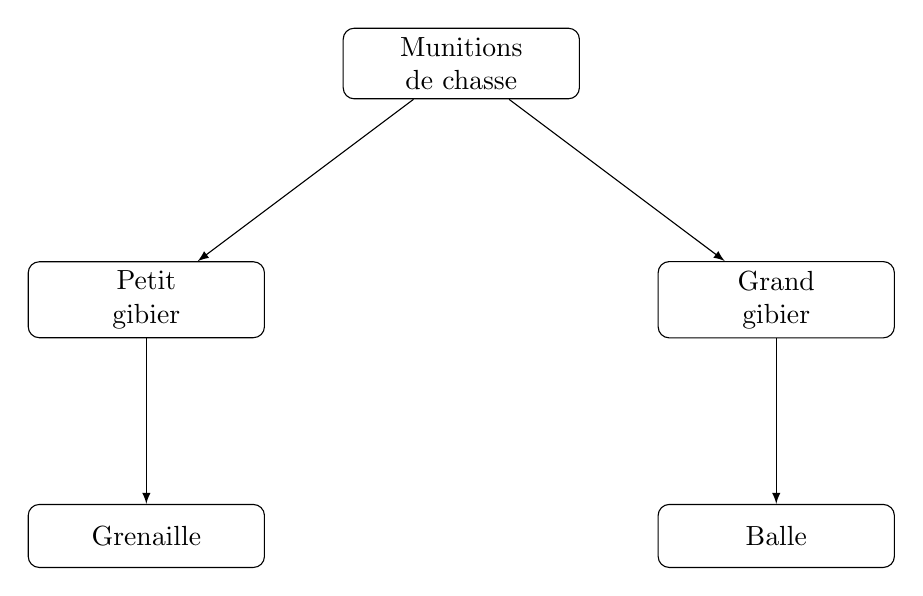
\begin{tikzpicture}[
every node/.style={
draw,
rounded corners,
align=center,
minimum width=3cm,
minimum height=8mm
}
]

\node (M) at (0,0) {Munitions\\de chasse};

\node (P) at (-4,-3) {Petit\\gibier};
\node (G) at (4,-3) {Grand\\gibier};

\node (Gr) at (-4,-6) {Grenaille};
\node (Ba) at (4,-6) {Balle};

\draw[-latex] (M) -- (P);
\draw[-latex] (M) -- (G);

\draw[-latex] (P) -- (Gr);
\draw[-latex] (G) -- (Ba);

\end{tikzpicture}

\caption{Exemples de munitions couramment utilisées selon le type de gibier.}
\label{fig:petit_grand_gibier}

\end{figure}

\section{Le petit gibier}

Le petit gibier comprend notamment :

\begin{itemize}
    \item certains oiseaux ;
    \item les lapins ;
    \item les lièvres ;
    \item divers petits mammifères.
\end{itemize}

Les cartouches à grenaille sont très largement utilisées dans ce domaine.

\section{Le grand gibier}

Le grand gibier regroupe notamment :

\begin{itemize}
    \item les sangliers ;
    \item les cervidés ;
    \item certains grands mammifères.
\end{itemize}

Les tirs sont généralement réalisés avec des projectiles uniques.

\section{Les cartouches à balle}

Les cartouches à balle utilisent un projectile unique.

Elles offrent généralement :

\begin{itemize}
    \item une meilleure portée ;
    \item une précision supérieure ;
    \item une énergie importante.
\end{itemize}

Elles sont principalement employées pour le grand gibier.

\section{Les cartouches à grenaille}

Les cartouches à grenaille contiennent un grand nombre de petits projectiles.

Après la sortie du canon, ceux-ci se dispersent progressivement.

Cette dispersion augmente les chances d'atteindre une cible de petite taille en
mouvement.

\begin{figure}[htbp]
\centering

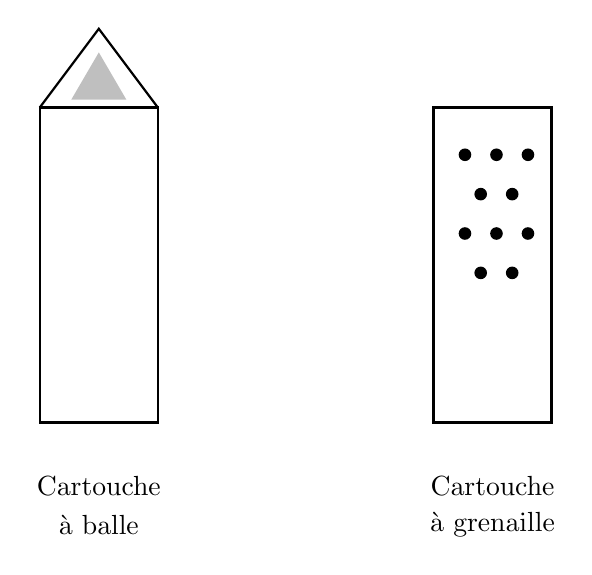
\begin{tikzpicture}[scale=1]

% Cartouche à balle
\draw[thick] (0,0) rectangle (1.5,4);
\draw[thick] (0,4) -- (0.75,5) -- (1.5,4);

\fill[gray!50] (0.4,4.1) -- (0.75,4.7) -- (1.1,4.1) -- cycle;

\node at (0.75,-0.8) {Cartouche};
\node at (0.75,-1.3) {à balle};

% Cartouche à grenaille
\begin{scope}[xshift=5cm]

\draw[thick] (0,0) rectangle (1.5,4);

\foreach \x/\y in {
0.4/3.4,0.8/3.4,1.2/3.4,
0.6/2.9,1.0/2.9,
0.4/2.4,0.8/2.4,1.2/2.4,
0.6/1.9,1.0/1.9
}
{
\fill (\x,\y) circle (0.08);
}

\node at (0.75,-0.8) {Cartouche};
\node at (0.75,-1.3) {à grenaille};

\end{scope}

\end{tikzpicture}

\caption{Comparaison simplifiée entre une cartouche à balle et une cartouche à grenaille.}
\label{fig:balle_grenaille}

\end{figure}

\section{La gerbe de plomb}

L'ensemble des projectiles dispersés est appelé :

\begin{quote}
gerbe
\end{quote}

La forme et la densité de cette gerbe influencent fortement l'efficacité du
tir.

\section{Influence de la distance}

Lorsque la distance augmente :

\begin{itemize}
    \item la gerbe s'élargit ;
    \item la densité d'impacts diminue ;
    \item l'énergie individuelle des projectiles diminue.
\end{itemize}

Le choix de la cartouche dépend donc fortement de la distance prévue.

\begin{figure}[htbp]
\centering

\begin{tikzpicture}[scale=1]

% Canon
\draw[thick] (0,0) -- (0,5);

\node[left] at (0,2.5) {Canon};

% Gerbes
\draw[dashed] (0,2.5) -- (3,3);
\draw[dashed] (0,2.5) -- (3,2);

\draw[dashed] (0,2.5) -- (6,4);
\draw[dashed] (0,2.5) -- (6,1);

\draw[dashed] (0,2.5) -- (9,5);
\draw[dashed] (0,2.5) -- (9,0);

% Distances
\draw (3,1.8) -- (3,3.2);
\node[below] at (3,1.8) {Courte};

\draw (6,0.8) -- (6,4.2);
\node[below] at (6,0.8) {Moyenne};

\draw (9,-0.2) -- (9,5.2);
\node[below] at (9,-0.2) {Longue};

\end{tikzpicture}

\caption{La gerbe s'élargit progressivement avec la distance.}
\label{fig:gerbe_distance}

\end{figure}

\section{Le calibre}

Dans le domaine du fusil de chasse, la notion de calibre diffère souvent de
celle rencontrée pour les armes rayées.

Les désignations les plus connues sont notamment :

\begin{itemize}
    \item calibre 12 ;
    \item calibre 16 ;
    \item calibre 20 ;
    \item calibre 28.
\end{itemize}

Leur signification sera étudiée plus loin dans l'ouvrage.

\section{La longueur de la chambre}

Les cartouches de chasse existent en plusieurs longueurs.

Le choix de la cartouche doit être compatible avec la chambre de l'arme.

\section{Les projectiles modernes}

Les projectiles de chasse modernes utilisent de nombreuses technologies :

\begin{itemize}
    \item noyaux plomb ;
    \item projectiles monolithiques ;
    \item conceptions expansives ;
    \item géométries optimisées.
\end{itemize}

\section{Expansion contrôlée}

De nombreuses balles de chasse sont conçues pour se déformer de manière
contrôlée après impact.

Cette déformation vise à améliorer le transfert d'énergie vers la cible.

\section{Préservation de la venaison}

Le chasseur cherche généralement à concilier :

\begin{itemize}
    \item efficacité ;
    \item sécurité ;
    \item préservation de la venaison.
\end{itemize}

Le choix du projectile influence directement ces critères.

\section{Sécurité}

La sécurité constitue un aspect fondamental de la chasse.

Le tireur doit tenir compte :

\begin{itemize}
    \item de son environnement ;
    \item de la portée potentielle du projectile ;
    \item des risques de ricochet ;
    \item de la présence éventuelle d'autres personnes.
\end{itemize}

\section{Évolution des réglementations}

Les réglementations relatives aux munitions de chasse évoluent régulièrement.

Certaines restrictions concernent notamment :

\begin{itemize}
    \item les matériaux utilisés ;
    \item les zones de chasse ;
    \item les espèces concernées.
\end{itemize}

\section{Vers les projectiles de chasse}

Les munitions de chasse utilisent une grande variété de projectiles adaptés à
des usages spécifiques.

Le chapitre suivant examinera plus en détail les principales familles de
projectiles utilisées dans ce domaine.

\begin{figure}[htbp]
\centering

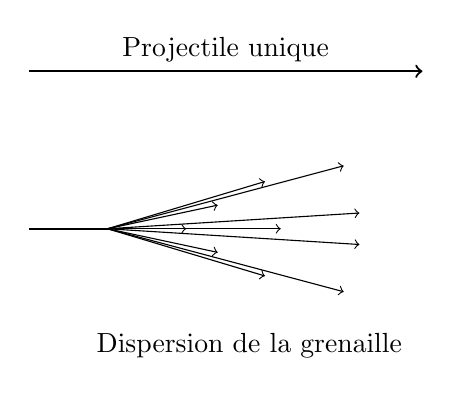
\begin{tikzpicture}[scale=1]

% Balle
\draw[thick,->] (0,0) -- (5,0);
\node[above] at (2.5,0) {Projectile unique};

% Grenaille
\begin{scope}[yshift=-2cm]

\draw[thick] (0,0) -- (1,0);

\foreach \x/\y in {
2/0,
2.4/0.3,
2.4/-0.3,
3/0.6,
3/-0.6,
3.2/0,
4/0.8,
4/-0.8,
4.2/0.2,
4.2/-0.2
}
{
\draw[->] (1,0) -- (\x,\y);
}

\node[below] at (2.8,-1.2) {Dispersion de la grenaille};

\end{scope}

\end{tikzpicture}

\caption{Différence de comportement entre un projectile unique et une charge de grenaille.}
\label{fig:balle_vs_grenaille}

\end{figure}

\section{À retenir}

\begin{aretenir}

\begin{itemize}
    \item Les munitions de chasse sont adaptées au type de gibier recherché.
    \item Les cartouches à balle et les cartouches à grenaille répondent à des
          besoins différents.
    \item La distance de tir influence fortement l'efficacité.
    \item Les projectiles modernes utilisent des conceptions variées.
    \item La sécurité reste une priorité absolue.
\end{itemize}

\end{aretenir}


    \chapter{Les projectiles de chasse}
    \label{chap:projectiles_chasse}
    %==============================================================================
% Chapitre 54 - Les projectiles de chasse
%==============================================================================

\section{Introduction}

Les projectiles de chasse présentent une grande diversité de formes et de
conceptions.

Contrairement aux munitions militaires, leur objectif principal est
généralement de produire un effet terminal adapté au gibier recherché.

La déformation du projectile après impact constitue souvent un critère de
conception important.

\begin{aretenir}

Un projectile de chasse est généralement conçu pour transférer efficacement
son énergie à la cible.

\end{aretenir}

\section{Les objectifs recherchés}

Les concepteurs cherchent souvent à obtenir un compromis entre :

\begin{itemize}
    \item précision ;
    \item pénétration ;
    \item expansion ;
    \item conservation de masse ;
    \item sécurité.
\end{itemize}

Ces critères peuvent parfois être contradictoires.

\section{La balle blindée}

La balle blindée possède une chemise métallique entourant le noyau.

Bien qu'elle puisse être utilisée pour certaines applications spécifiques,
elle reste relativement peu employée à la chasse.

Sa déformation limitée réduit généralement le transfert d'énergie.

\section{La balle demi-blindée}

La balle demi-blindée constitue l'une des conceptions les plus répandues.

Une partie du noyau est laissée apparente à l'avant du projectile.

Cette configuration favorise l'expansion après impact.

\begin{figure}[htbp]
\centering

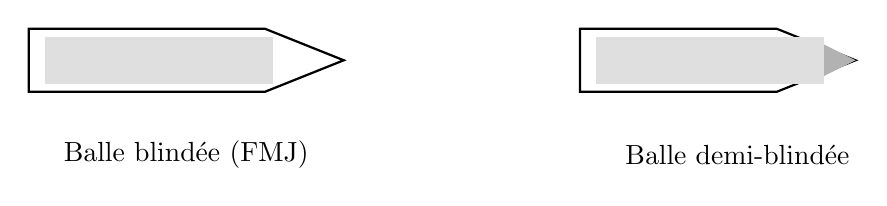
\begin{tikzpicture}[scale=1]

% FMJ
\draw[thick]
(0,0)
--
(0,0.8)
--
(3,0.8)
--
(4,0.4)
--
(3,0)
--
cycle;

\fill[gray!25]
(0.2,0.1)
rectangle
(3.1,0.7);

\node at (2,-0.8) {Balle blindée (FMJ)};

% Demi-blindée
\begin{scope}[xshift=7cm]

\draw[thick]
(0,0)
--
(0,0.8)
--
(2.5,0.8)
--
(3.5,0.4)
--
(2.5,0)
--
cycle;

\fill[gray!25]
(0.2,0.1)
rectangle
(3.1,0.7);

\fill[gray!60]
(3.1,0.2)
--
(3.5,0.4)
--
(3.1,0.6)
--
cycle;

\node at (2,-0.8) {Balle demi-blindée};

\end{scope}

\end{tikzpicture}

\caption{Comparaison simplifiée entre une balle blindée et une balle demi-blindée.}
\label{fig:fmj_demi_blindee}

\end{figure}

\section{Principe de l'expansion}

Lors de l'impact, la partie avant du projectile se déforme progressivement.

Cette déformation augmente généralement :

\begin{itemize}
    \item le diamètre apparent ;
    \item la surface de contact ;
    \item le transfert d'énergie.
\end{itemize}

\begin{figure}[htbp]
\centering

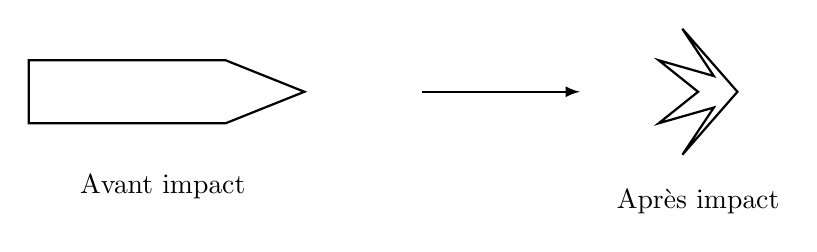
\begin{tikzpicture}[scale=1]

% Avant
\draw[thick]
(0,0)
--
(0,0.8)
--
(2.5,0.8)
--
(3.5,0.4)
--
(2.5,0)
--
cycle;

\node at (1.7,-0.8) {Avant impact};

% Flèche
\draw[-latex,thick]
(5,0.4)
--
(7,0.4);

% Après
\draw[thick]
(9,0.4)
--
(8.3,1.2)
--
(8.7,0.6)
--
(8,0.8)
--
(8.5,0.4)
--
(8,0)
--
(8.7,0.2)
--
(8.3,-0.4)
--
cycle;

\node at (8.5,-1.0) {Après impact};

\end{tikzpicture}

\caption{Principe simplifié de l'expansion d'une balle de chasse.}
\label{fig:expansion_balle}

\end{figure}

\section{La balle à pointe creuse}

La balle à pointe creuse comporte une cavité située à l'avant.

Cette cavité facilite l'ouverture du projectile lors de l'impact.

\begin{figure}[htbp]
\centering

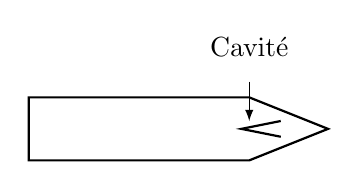
\begin{tikzpicture}[scale=1]

\draw[thick]
(0,0)
--
(0,0.8)
--
(2.8,0.8)
--
(3.8,0.4)
--
(2.8,0)
--
cycle;

% Cavité
\draw[thick]
(3.2,0.3)
--
(2.7,0.4)
--
(3.2,0.5);

\node[above] at (2.8,1.2)
{Cavité};

\draw[-latex]
(2.8,1.0)
--
(2.8,0.5);

\end{tikzpicture}

\caption{Coupe simplifiée d'une balle à pointe creuse.}
\label{fig:pointe_creuse}

\end{figure}

\section{La balle à pointe polymère}

Certaines conceptions modernes utilisent une pointe en matériau polymère.

Cette pointe améliore souvent :

\begin{itemize}
    \item l'aérodynamique ;
    \item la régularité de l'expansion ;
    \item la précision.
\end{itemize}

\section{Les projectiles monolithiques}

Les projectiles monolithiques sont réalisés dans un seul matériau.

Ils sont souvent usinés à partir d'un alliage métallique.

\section{Conservation de masse}

Lors de l'impact, certains projectiles peuvent perdre une partie de leur
masse.

D'autres sont conçus pour conserver une proportion importante de leur masse
initiale.

Cette caractéristique influence directement la pénétration.

\section{Expansion contrôlée}

Les projectiles modernes cherchent souvent à limiter les comportements
imprévisibles.

L'expansion contrôlée vise à obtenir une déformation régulière et
reproductible.

\section{Pénétration}

Une pénétration suffisante demeure indispensable.

Un projectile qui s'expanse trop rapidement risque de ne pas atteindre les
organes recherchés.

\section{Compromis expansion-pénétration}

L'expansion et la pénétration constituent souvent deux objectifs opposés.

Une expansion importante tend à augmenter le transfert d'énergie mais peut
réduire la profondeur de pénétration.

\begin{figure}[htbp]
\centering

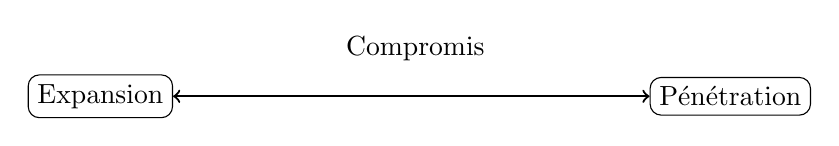
\begin{tikzpicture}[scale=1]

\node[draw,rounded corners]
(E)
at (0,0)
{Expansion};

\node[draw,rounded corners]
(P)
at (8,0)
{Pénétration};

\draw[<->,thick]
(E)
--
(P);

\node
at (4,0.6)
{Compromis};

\end{tikzpicture}

\caption{L'expansion et la pénétration constituent souvent des objectifs contradictoires.}
\label{fig:compromis_expansion_penetration}

\end{figure}

\section{Influence de la vitesse}

Le comportement terminal dépend fortement de la vitesse d'impact.

Un même projectile peut présenter des résultats différents selon :

\begin{itemize}
    \item la distance ;
    \item la vitesse résiduelle ;
    \item la nature de la cible.
\end{itemize}

\section{Le choix du projectile}

Le choix dépend notamment :

\begin{itemize}
    \item du gibier ;
    \item de la distance de tir ;
    \item du calibre ;
    \item de la réglementation.
\end{itemize}

\section{Évolution récente}

Les progrès des matériaux et des procédés de fabrication ont permis le
développement de projectiles de plus en plus spécialisés.

Les performances obtenues aujourd'hui étaient difficilement envisageables il y
a quelques décennies.

\section{Vers les cartouches de chasse}

Le projectile ne constitue qu'un élément de la munition.

Le chapitre suivant examinera plus en détail la structure complète des
cartouches de chasse modernes.

\begin{figure}[htbp]
\centering

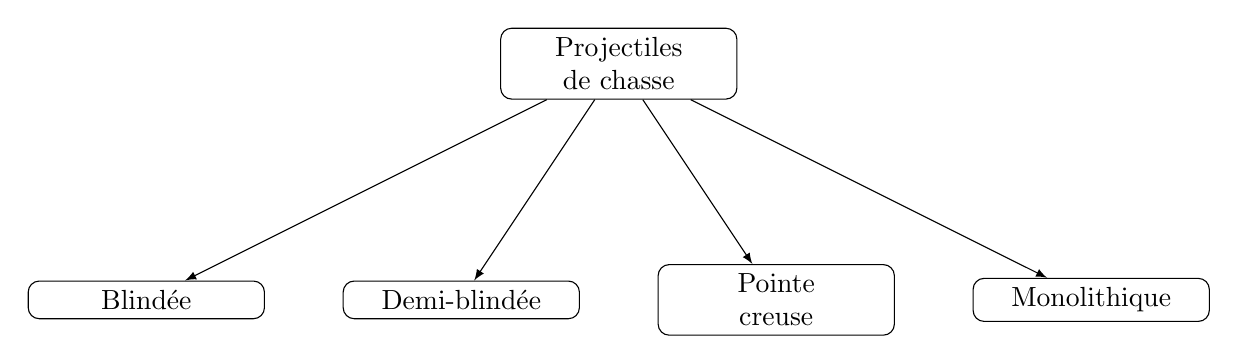
\begin{tikzpicture}[
every node/.style={
draw,
rounded corners,
align=center,
minimum width=3cm
}
]

\node (P) at (0,0) {Projectiles\\de chasse};

\node (F) at (-6,-3) {Blindée};
\node (D) at (-2,-3) {Demi-blindée};
\node (C) at (2,-3) {Pointe\\creuse};
\node (M) at (6,-3) {Monolithique};

\draw[-latex] (P) -- (F);
\draw[-latex] (P) -- (D);
\draw[-latex] (P) -- (C);
\draw[-latex] (P) -- (M);

\end{tikzpicture}

\caption{Principales familles de projectiles de chasse modernes.}
\label{fig:familles_projectiles_chasse}

\end{figure}

\section{À retenir}

\begin{aretenir}

\begin{itemize}
    \item Les projectiles de chasse sont conçus pour produire un effet terminal
          adapté.
    \item La balle demi-blindée reste très répandue.
    \item L'expansion contrôlée constitue un objectif majeur.
    \item La pénétration et l'expansion doivent être équilibrées.
    \item Les conceptions modernes utilisent des matériaux et géométries
          variés.
\end{itemize}

\end{aretenir}


    \chapter{Structure d'une cartouche de chasse}
    \label{chap:structure_cartouche_chasse}
    %==============================================================================
% Chapitre 55 - Structure d'une cartouche de chasse
%==============================================================================

\section{Introduction}

La cartouche de chasse moderne possède une architecture particulière qui
diffère sensiblement des cartouches métalliques utilisées dans les armes
rayées.

Elle est généralement constituée de plusieurs éléments superposés assurant
chacun une fonction spécifique.

\begin{aretenir}

Une cartouche de chasse est un système complet dans lequel chaque composant
participe aux performances du tir.

\end{aretenir}

\section{Vue d'ensemble}

Une cartouche de chasse moderne comprend généralement :

\begin{itemize}
    \item une douille ;
    \item une amorce ;
    \item une charge de poudre ;
    \item une bourre ;
    \item une charge de projectiles ;
    \item un sertissage.
\end{itemize}

\begin{figure}[htbp]
\centering

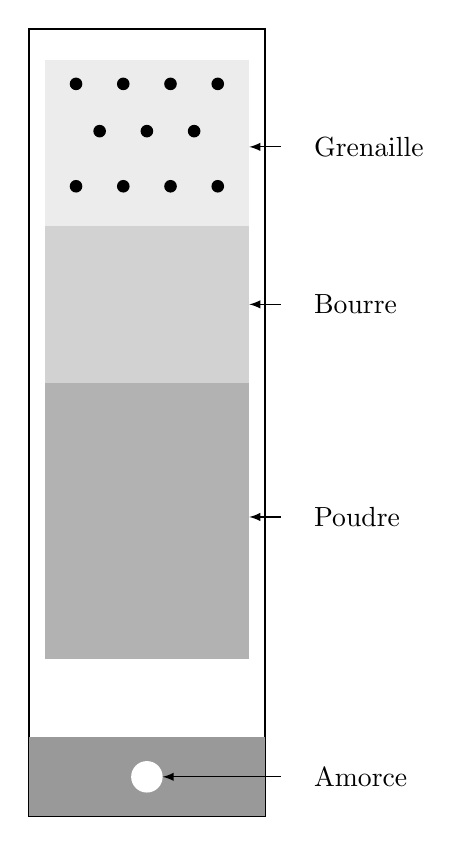
\begin{tikzpicture}[scale=1]

% Douille
\draw[thick] (0,0) rectangle (3,10);

% Grenaille
\fill[gray!15] (0.2,7.5) rectangle (2.8,9.6);

\foreach \x/\y in {
0.6/8.0,1.2/8.0,1.8/8.0,2.4/8.0,
0.9/8.7,1.5/8.7,2.1/8.7,
0.6/9.3,1.2/9.3,1.8/9.3,2.4/9.3
}
{
\fill (\x,\y) circle (0.08);
}

% Bourre
\fill[gray!35] (0.2,5.5) rectangle (2.8,7.5);

% Poudre
\fill[gray!60] (0.2,2.0) rectangle (2.8,5.5);

% Culot
\fill[gray!80] (0,0) rectangle (3,1);

% Amorce
\fill[white] (1.5,0.5) circle (0.2);

% Légendes
\node[right] at (3.5,8.5) {Grenaille};
\node[right] at (3.5,6.5) {Bourre};
\node[right] at (3.5,3.8) {Poudre};
\node[right] at (3.5,0.5) {Amorce};

\draw[-latex] (3.2,8.5) -- (2.8,8.5);
\draw[-latex] (3.2,6.5) -- (2.8,6.5);
\draw[-latex] (3.2,3.8) -- (2.8,3.8);
\draw[-latex] (3.2,0.5) -- (1.7,0.5);

\end{tikzpicture}

\caption{Coupe simplifiée d'une cartouche de chasse à grenaille.}
\label{fig:cartouche_chasse_grenaille}

\end{figure}

\section{La douille}

La douille constitue l'enveloppe principale de la cartouche.

Elle assure notamment :

\begin{itemize}
    \item le maintien des composants ;
    \item l'étanchéité des gaz ;
    \item l'alimentation de l'arme.
\end{itemize}

\section{Le culot métallique}

La partie inférieure de la cartouche comporte généralement un culot métallique.

Celui-ci renforce la zone soumise aux efforts les plus importants lors du tir.

\section{L'amorce}

L'amorce est située au centre du culot.

Elle initie la combustion de la poudre lorsque le percuteur la frappe.

\section{La poudre}

La poudre constitue la source d'énergie de la cartouche.

Sa combustion produit les gaz nécessaires à la propulsion de la charge.

\section{La bourre}

La bourre est un élément essentiel des cartouches de chasse.

Elle remplit plusieurs fonctions :

\begin{itemize}
    \item séparation de la poudre et des projectiles ;
    \item transmission de la poussée ;
    \item protection de la charge ;
    \item influence sur la gerbe.
\end{itemize}

\section{Les bourres traditionnelles}

Historiquement, les bourres étaient réalisées dans différents matériaux :

\begin{itemize}
    \item feutre ;
    \item carton ;
    \item fibres végétales.
\end{itemize}

\section{Les bourres modernes}

Les bourres modernes utilisent souvent des matériaux synthétiques.

Elles permettent un meilleur contrôle du comportement de la charge.

\begin{figure}[htbp]
\centering

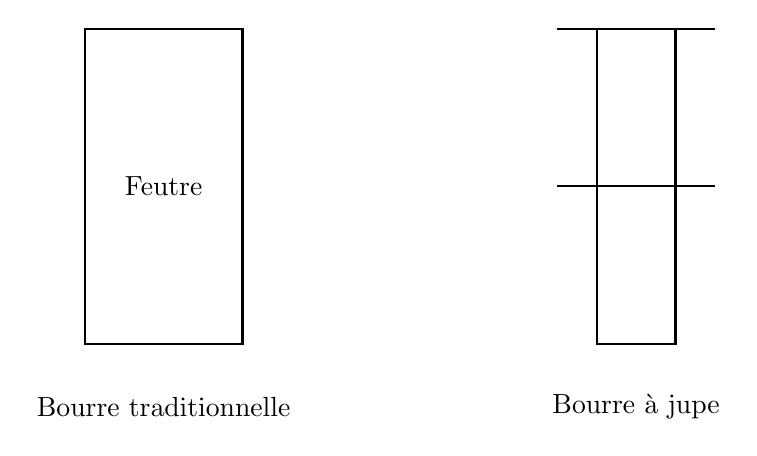
\begin{tikzpicture}[scale=1]

% Bourre feutre
\draw[thick] (0,0) rectangle (2,4);

\node at (1,2) {Feutre};

\node at (1,-0.8)
{Bourre traditionnelle};

% Bourre moderne
\begin{scope}[xshift=6cm]

\draw[thick] (0.5,0) rectangle (1.5,4);

\draw[thick] (0,2) -- (2,2);
\draw[thick] (0,4) -- (0.5,4);
\draw[thick] (1.5,4) -- (2,4);

\node at (1,-0.8)
{Bourre à jupe};

\end{scope}

\end{tikzpicture}

\caption{Exemple simplifié de bourres utilisées dans les cartouches de chasse.}
\label{fig:bourres_chasse}

\end{figure}

\section{La charge de projectiles}

Selon le type de munition, la charge peut être constituée :

\begin{itemize}
    \item d'une balle unique ;
    \item de chevrotines ;
    \item de grenaille.
\end{itemize}

\section{Le sertissage}

Le sertissage ferme l'extrémité avant de la cartouche.

Il assure le maintien de la charge avant le tir.

\section{Influence du sertissage}

Le sertissage influence notamment :

\begin{itemize}
    \item la pression ;
    \item la régularité ;
    \item le départ de la charge.
\end{itemize}

\begin{figure}[htbp]
\centering

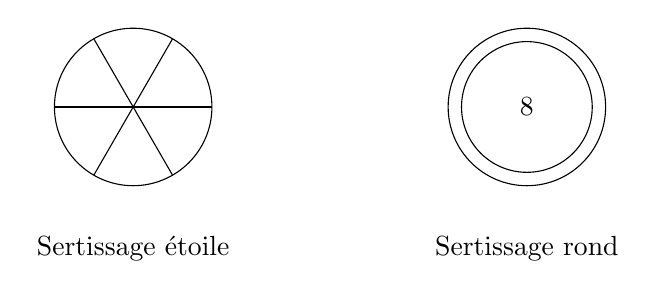
\begin{tikzpicture}[scale=1]

% Etoile
\draw (0,0) circle (1);

\foreach \a in {0,60,120,180,240,300}
{
\draw (0,0) -- (\a:1);
}

\node at (0,-1.8)
{Sertissage étoile};

% Rond
\begin{scope}[xshift=5cm]

\draw (0,0) circle (1);

\draw (0,0) circle (0.83);

\node at (0,0)
{8};

\node at (0,-1.8)
{Sertissage rond};

\end{scope}

\end{tikzpicture}

\caption{Exemples de sertissages couramment rencontrés.}
\label{fig:sertissages}

\end{figure}

\section{Longueur de la cartouche}

La longueur indiquée sur les cartouches de chasse correspond généralement à la
longueur après ouverture complète du sertissage.

Cette particularité peut surprendre les débutants.

\section{Compatibilité avec la chambre}

Une cartouche doit toujours être compatible avec la chambre de l'arme.

Le respect de cette compatibilité constitue une exigence de sécurité
fondamentale.

\section{Cartouches à grenaille}

Dans les cartouches à grenaille, la charge est constituée d'un grand nombre de
petits projectiles.

Leur organisation interne influence la qualité de la gerbe.

\section{Cartouches à balle}

Les cartouches à balle utilisent un projectile unique.

Leur structure générale reste néanmoins proche de celle des cartouches à
grenaille.

\begin{figure}[htbp]
\centering

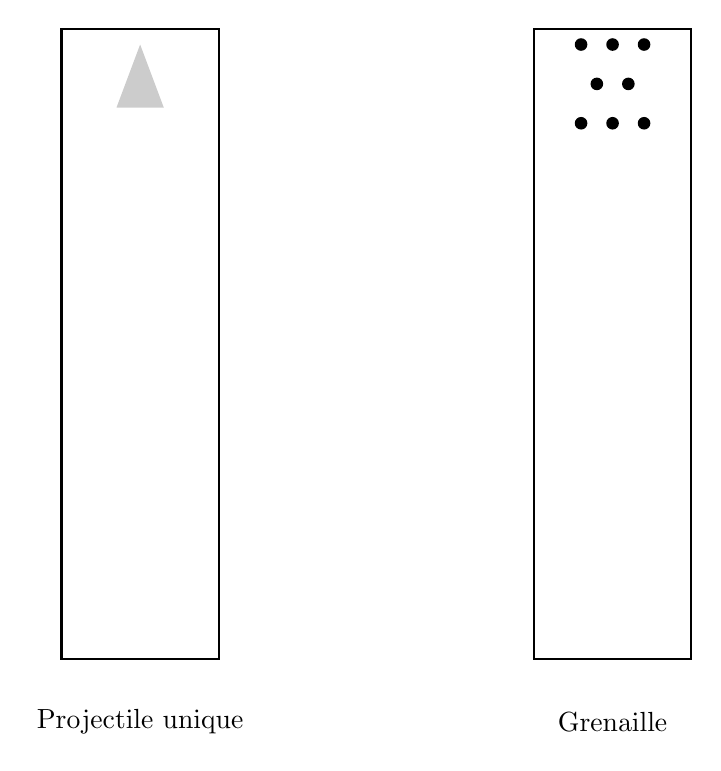
\begin{tikzpicture}[scale=1]

% Cartouche balle
\draw[thick] (0,0) rectangle (2,8);

\fill[gray!40]
(0.7,7)
--
(1,7.8)
--
(1.3,7)
--
cycle;

\node at (1,-0.8)
{Projectile unique};

% Cartouche grenaille
\begin{scope}[xshift=6cm]

\draw[thick] (0,0) rectangle (2,8);

\foreach \x/\y in {
0.6/6.8,1.0/6.8,1.4/6.8,
0.8/7.3,1.2/7.3,
0.6/7.8,1.0/7.8,1.4/7.8
}
{
\fill (\x,\y) circle (0.08);
}

\node at (1,-0.8)
{Grenaille};

\end{scope}

\end{tikzpicture}

\caption{Comparaison simplifiée entre une cartouche à balle et une cartouche à grenaille.}
\label{fig:balle_ou_grenaille}

\end{figure}


\section{Évolution des conceptions}

Les progrès des matériaux et des procédés industriels ont permis de faire
évoluer les cartouches de chasse tout en conservant leur architecture
générale.

\section{Vers les bourres et les chokes}

Parmi les composants d'une cartouche de chasse, la bourre joue un rôle
particulièrement important.

Les prochains chapitres examineront plus en détail son influence ainsi que
celle des chokes.

\section{À retenir}

\begin{aretenir}

\begin{itemize}
    \item Une cartouche de chasse est constituée de plusieurs éléments
          complémentaires.
    \item La bourre joue un rôle essentiel.
    \item Le sertissage influence le comportement de la cartouche.
    \item Les cartouches à balle et à grenaille partagent une architecture
          similaire.
    \item La compatibilité avec la chambre est indispensable.
\end{itemize}

\end{aretenir}


    \chapter{Les bourres}
    \label{chap:les_bourres}
    %==============================================================================
% Chapitre 56 - Les bourres
%==============================================================================

\section{Introduction}

La bourre constitue l'un des éléments les plus importants d'une cartouche de
chasse.

Bien que souvent méconnue du grand public, elle influence fortement le
comportement de la munition et la qualité de la gerbe.

\begin{aretenir}

La bourre transmet l'énergie de la poudre à la charge tout en influençant la
dispersion des projectiles.

\end{aretenir}

\section{Position dans la cartouche}

La bourre est située entre la poudre et la charge de projectiles.

Elle constitue l'interface mécanique entre les gaz produits par la combustion
et la charge propulsée.

\begin{figure}[htbp]
\centering

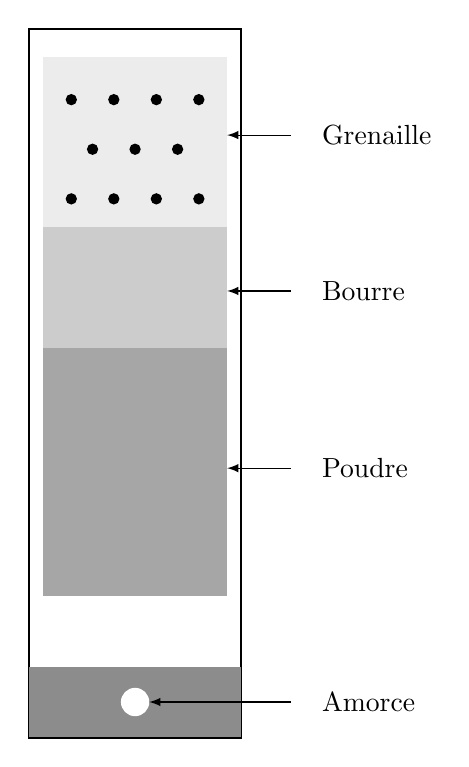
\begin{tikzpicture}[scale=0.9]

% Douille
\draw[thick] (0,0) rectangle (3,10);

% Grenaille
\fill[gray!15] (0.2,7.2) rectangle (2.8,9.6);

\foreach \x/\y in {
0.6/7.6,1.2/7.6,1.8/7.6,2.4/7.6,
0.9/8.3,1.5/8.3,2.1/8.3,
0.6/9.0,1.2/9.0,1.8/9.0,2.4/9.0
}
{
\fill (\x,\y) circle (0.08);
}

% Bourre
\fill[gray!40] (0.2,5.5) rectangle (2.8,7.2);

% Poudre
\fill[gray!70] (0.2,2.0) rectangle (2.8,5.5);

% Culot
\fill[gray!90] (0,0) rectangle (3,1);

% Amorce
\fill[white] (1.5,0.5) circle (0.2);

\node[right] at (4,8.5) {Grenaille};
\node[right] at (4,6.3) {Bourre};
\node[right] at (4,3.8) {Poudre};
\node[right] at (4,0.5) {Amorce};

\draw[-latex] (3.7,8.5) -- (2.8,8.5);
\draw[-latex] (3.7,6.3) -- (2.8,6.3);
\draw[-latex] (3.7,3.8) -- (2.8,3.8);
\draw[-latex] (3.7,0.5) -- (1.7,0.5);

\end{tikzpicture}

\caption{Position de la bourre dans une cartouche de chasse.}
\label{fig:position_bourre}

\end{figure}

\section{Fonctions principales}

La bourre remplit plusieurs fonctions simultanément :

\begin{itemize}
    \item transmettre la poussée ;
    \item assurer l'étanchéité ;
    \item protéger les projectiles ;
    \item influencer la gerbe ;
    \item amortir certaines contraintes mécaniques.
\end{itemize}

\section{Transmission de la poussée}

Lors du tir, les gaz produits par la poudre exercent une pression importante.

La bourre transmet cette pression à la charge de manière efficace.

\section{Étanchéité}

Une bonne étanchéité limite les pertes de gaz.

Elle contribue directement au rendement de la cartouche.

\section{Protection des projectiles}

La bourre protège les projectiles du contact direct avec les parois du canon.

Cette fonction est particulièrement importante avec les bourres modernes à
jupe.

\section{Les bourres traditionnelles}

Pendant longtemps, les bourres étaient réalisées dans des matériaux naturels.

On utilisait notamment :

\begin{itemize}
    \item le feutre ;
    \item le carton ;
    \item le liège ;
    \item certaines fibres végétales.
\end{itemize}

\section{Les bourres grasses}

La bourre grasse est une forme classique de bourre traditionnelle.

Elle est généralement constituée de feutre ou de matériaux similaires.

\section{Les bourres modernes}

Les bourres modernes sont généralement fabriquées en matière synthétique.

Elles offrent des performances plus régulières.

\section{La bourre à jupe}

La bourre à jupe est devenue très répandue.

Elle entoure partiellement la charge de grenaille et limite les contacts avec
le canon.

\begin{figure}[htbp]
\centering

\begin{tikzpicture}

% Bourre grasse
\draw[thick] (0,0) rectangle (2,4);

\node at (1,2) {Feutre};

\node at (1,-0.8)
{Bourre grasse};

% Bourre à jupe
\begin{scope}[xshift=7cm]

\draw[thick] (0.7,0) rectangle (1.3,4);

\draw[thick] (0,2) -- (2,2);

\draw[thick] (0,4) -- (0.7,4);
\draw[thick] (1.3,4) -- (2,4);

\node at (1,-0.8)
{Bourre à jupe};

\end{scope}

\end{tikzpicture}

\caption{Comparaison simplifiée entre une bourre grasse et une bourre à jupe.}
\label{fig:bourre_grasse_jupe}

\end{figure}

\section{Protection de la gerbe}

En limitant les déformations des projectiles, la bourre à jupe contribue à
maintenir une gerbe plus homogène.

\begin{figure}[htbp]
\centering

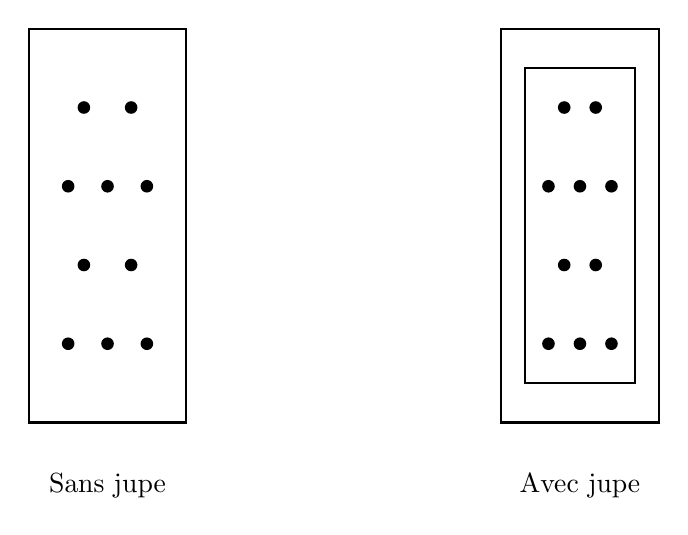
\begin{tikzpicture}[scale=1]

% Sans jupe
\draw[thick] (0,0) rectangle (2,5);

\foreach \x/\y in {
0.5/1,1.0/1,1.5/1,
0.7/2,1.3/2,
0.5/3,1.0/3,1.5/3,
0.7/4,1.3/4
}
{
\fill (\x,\y) circle (0.08);
}

\node at (1,-0.8) {Sans jupe};

% Avec jupe
\begin{scope}[xshift=6cm]

\draw[thick] (0,0) rectangle (2,5);

\draw[thick] (0.3,0.5) rectangle (1.7,4.5);

\foreach \x/\y in {
0.6/1,1.0/1,1.4/1,
0.8/2,1.2/2,
0.6/3,1.0/3,1.4/3,
0.8/4,1.2/4
}
{
\fill (\x,\y) circle (0.08);
}

\node at (1,-0.8) {Avec jupe};

\end{scope}

\end{tikzpicture}

\caption{La bourre à jupe limite le contact direct entre la grenaille et le canon.}
\label{fig:protection_grenaille}

\end{figure}

\section{Séparation après la bouche}

Après la sortie du canon, la bourre poursuit brièvement sa trajectoire.

Elle se sépare ensuite de la charge de projectiles.

\begin{figure}[htbp]
\centering

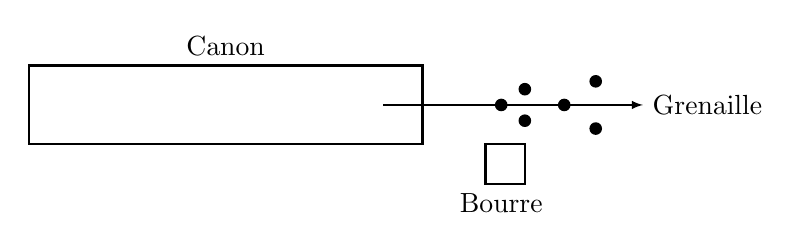
\begin{tikzpicture}[scale=1]

% Canon
\draw[thick] (0,1) rectangle (5,2);

\node[above] at (2.5,2)
{Canon};

% Charge
\foreach \x/\y in {
6/1.5,
6.3/1.7,
6.3/1.3,
6.8/1.5,
7.2/1.8,
7.2/1.2
}
{
\fill (\x,\y) circle (0.08);
}

% Bourre
\draw[thick]
(5.8,0.5)
rectangle
(6.3,1.0);

% Flèches
\draw[-latex] (4.5,1.5) -- (7.8,1.5);

\node[right] at (7.8,1.5)
{Grenaille};

\node[below] at (6.0,0.5)
{Bourre};

\end{tikzpicture}

\caption{Après la sortie du canon, la bourre se sépare progressivement de la charge.}
\label{fig:separation_bourre}

\end{figure}

\section{Influence sur la dispersion}

La conception de la bourre influence directement :

\begin{itemize}
    \item la densité de la gerbe ;
    \item la régularité des impacts ;
    \item la dispersion.
\end{itemize}

\section{Compatibilité avec les chokes}

Le comportement de la bourre dépend également du choke utilisé.

L'interaction entre ces deux éléments influence fortement les résultats en
cible.

\section{Applications selon le type de chasse}

Certaines bourres sont privilégiées pour les tirs à courte distance.

D'autres sont davantage adaptées aux tirs plus lointains.

Le choix dépend donc de l'usage recherché.

\section{Évolution des matériaux}

Les préoccupations environnementales ont conduit au développement de nouvelles
solutions.

Les matériaux utilisés continuent d'évoluer.

\section{Vers les chokes}

La bourre influence fortement la gerbe, mais elle n'est pas le seul élément en
cause.

Le chapitre suivant présentera les chokes et leur rôle dans le contrôle de la
dispersion.

\begin{figure}[htbp]
\centering

\begin{tikzpicture}

% Bourre grasse
\node at (0,4) {Bourre grasse};

\draw[dashed] (0,0) ellipse (2.2 and 1.3);

\foreach \x/\y in {
-1.2/0.6,-0.7/0.9,0.1/0.5,1.1/0.6,
-1.3/-0.5,-0.2/-0.8,0.9/-0.6,
0.0/0.0,0.6/0.1,-0.6/0.2
}
{
\fill (\x,\y) circle (0.06);
}

% Bourre à jupe
\begin{scope}[xshift=8cm]

\node at (0,4) {Bourre à jupe};

\draw[dashed] (0,0) ellipse (1.2 and 0.8);

\foreach \x/\y in {
-0.4/0.2,-0.2/0.4,0.0/0.1,
0.3/0.3,0.5/0.0,-0.3/-0.2,
0.2/-0.3,0.0/0.0,0.4/-0.1,
-0.5/0.0
}
{
\fill (\x,\y) circle (0.06);
}

\end{scope}

\end{tikzpicture}

\caption{Influence simplifiée de la bourre sur la dispersion de la gerbe.}
\label{fig:influence_bourre_gerbe}

\end{figure}

\section{À retenir}

\begin{aretenir}

\begin{itemize}
    \item La bourre assure plusieurs fonctions simultanément.
    \item Elle transmet la poussée des gaz à la charge.
    \item Les bourres à jupe protègent efficacement les projectiles.
    \item La bourre influence directement la gerbe.
    \item Son comportement dépend également du choke utilisé.
\end{itemize}

\end{aretenir}


    \chapter{Les chokes}
    \label{chap:les_chokes}
    %==============================================================================
% Chapitre 57 - Les chokes
%==============================================================================

\section{Introduction}

Les chokes sont des dispositifs destinés à modifier la dispersion des
projectiles dans les armes à canon lisse.

Ils jouent un rôle important dans les performances des fusils de chasse.

Leur influence est particulièrement visible avec les cartouches à grenaille.

\begin{aretenir}

Un choke modifie la dispersion de la gerbe en agissant sur la sortie de la
charge à la bouche du canon.

\end{aretenir}

\section{Principe général}

Un choke correspond à un léger rétrécissement situé à l'extrémité du canon.

Ce rétrécissement agit sur la charge lors de son passage.

L'objectif recherché est généralement de contrôler la dispersion de la gerbe.

\begin{figure}[htbp]
\centering

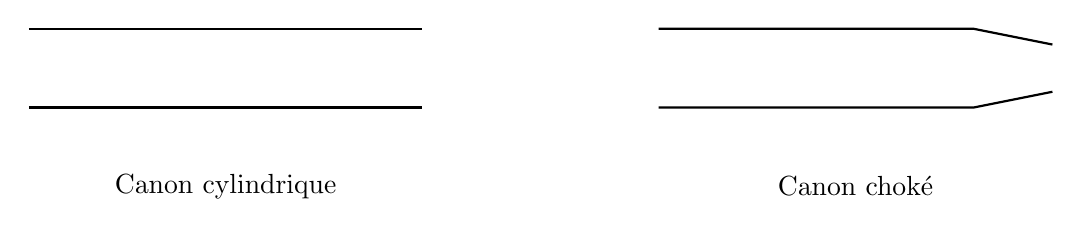
\begin{tikzpicture}[scale=1]

% Canon cylindrique
\draw[thick] (0,1) -- (5,1);
\draw[thick] (0,0) -- (5,0);

\node at (2.5,-1)
{Canon cylindrique};

% Canon choké
\begin{scope}[xshift=8cm]

\draw[thick]
(0,1)
--
(4,1)
--
(5,0.8);

\draw[thick]
(0,0)
--
(4,0)
--
(5,0.2);

\node at (2.5,-1)
{Canon choké};

\end{scope}

\end{tikzpicture}

\caption{Principe simplifié d'un choke placé à l'extrémité du canon.}
\label{fig:principe_choke}

\end{figure}

\section{Pourquoi utiliser un choke ?}

Selon les situations de chasse, il peut être souhaitable d'obtenir :

\begin{itemize}
    \item une gerbe large ;
    \item une gerbe intermédiaire ;
    \item une gerbe dense.
\end{itemize}

Les chokes permettent d'adapter le comportement du fusil à l'usage recherché.

\section{Canon cylindrique}

Un canon cylindrique ne comporte pratiquement aucun rétrécissement.

La dispersion obtenue est généralement importante.

Cette configuration est souvent adaptée aux tirs à courte distance.

\section{Quart de choke}

Le quart de choke constitue un léger rétrécissement.

Il réduit modérément la dispersion.

\section{Demi-choke}

Le demi-choke représente un compromis très répandu.

Il offre un équilibre entre ouverture de la gerbe et concentration.

\section{Trois-quarts de choke}

Le trois-quarts de choke produit une gerbe généralement plus dense.

Il est souvent utilisé pour des tirs plus éloignés.

\section{Full choke}

Le full choke correspond à un rétrécissement plus important.

Il permet généralement d'obtenir la gerbe la plus concentrée parmi les
configurations classiques.

\begin{figure}[htbp]
\centering

\begin{tikzpicture}[scale=0.9]

% Cylindrique
\draw (0,1) -- (3,1);
\draw (0,0) -- (3,0);
\node at (1.5,-0.8) {Cyl.};

% 1/4
\begin{scope}[xshift=4cm]
\draw (0,1) -- (2.5,1) -- (3,0.9);
\draw (0,0) -- (2.5,0) -- (3,0.1);
\node at (1.5,-0.8) {1/4};
\end{scope}

% 1/2
\begin{scope}[xshift=8cm]
\draw (0,1) -- (2.2,1) -- (3,0.8);
\draw (0,0) -- (2.2,0) -- (3,0.2);
\node at (1.5,-0.8) {1/2};
\end{scope}

% 3/4
\begin{scope}[xshift=12cm]
\draw (0,1) -- (2,1) -- (3,0.7);
\draw (0,0) -- (2,0) -- (3,0.3);
\node at (1.5,-0.8) {3/4};
\end{scope}

% Full
\begin{scope}[xshift=16cm]
\draw (0,1) -- (1.8,1) -- (3,0.6);
\draw (0,0) -- (1.8,0) -- (3,0.4);
\node at (1.5,-0.8) {Full};
\end{scope}

\end{tikzpicture}

\caption{Illustration simplifiée des principaux niveaux de choke.}
\label{fig:niveaux_choke}

\end{figure}

\section{Influence sur la gerbe}

Lorsque le choke augmente :

\begin{itemize}
    \item la dispersion diminue ;
    \item la densité de la gerbe augmente ;
    \item la portée utile tend à augmenter.
\end{itemize}

\begin{figure}[htbp]
\centering

\begin{tikzpicture}

% Gerbe ouverte
\draw[dashed] (0,0) circle (2);

\foreach \x/\y in {
-1.3/0.7,-1.1/-0.5,-0.5/1.2,
0.4/1.0,1.2/0.6,1.0/-0.8,
0.0/0.0,-0.3/-1.2,0.6/-1.1,
-1.5/0.0,1.4/0.1
}
{
\fill (\x,\y) circle (0.06);
}

\node at (0,-3)
{Canon cylindrique};

% Gerbe dense
\begin{scope}[xshift=8cm]

\draw[dashed] (0,0) circle (2);

\foreach \x/\y in {
-0.5/0.4,-0.3/0.6,-0.1/0.2,
0.2/0.5,0.5/0.2,
-0.4/-0.3,-0.1/-0.5,
0.2/-0.4,0.5/-0.2,
0.0/0.0,0.1/0.1,
-0.2/0.1
}
{
\fill (\x,\y) circle (0.06);
}

\node at (0,-3)
{Full choke};

\end{scope}

\end{tikzpicture}

\caption{Influence simplifiée du choke sur la densité de la gerbe.}
\label{fig:gerbe_choke}

\end{figure}

\section{Distance de tir}

Le choix du choke dépend fortement de la distance prévue.

Un choke très serré peut être peu adapté à un tir très rapproché.

Inversement, un choke très ouvert peut devenir insuffisant à longue distance.

\section{Compatibilité avec les munitions}

Toutes les munitions ne réagissent pas de la même manière.

Le comportement dépend notamment :

\begin{itemize}
    \item de la grenaille ;
    \item de la bourre ;
    \item de la vitesse ;
    \item du diamètre des projectiles.
\end{itemize}

\section{Influence de la bourre}

La bourre et le choke agissent conjointement.

Le résultat final dépend de l'interaction entre ces deux éléments.

\section{Chokes fixes}

Pendant longtemps, les fusils utilisaient des chokes fixes usinés directement
dans le canon.

Le choix était alors permanent.

\section{Chokes interchangeables}

De nombreux fusils modernes utilisent des chokes démontables.

Cette solution offre davantage de flexibilité.

\begin{figure}[htbp]
\centering

\begin{tikzpicture}[scale=1]

% Canon
\draw[thick]
(0,0)
rectangle
(8,1);

% Choke
\draw[thick]
(8,0)
rectangle
(10,1);

% Filetage simplifié
\foreach \x in {8.2,8.4,8.6,8.8,9.0}
{
\draw (\x,0) -- (\x,1);
}

\node at (4,-0.8)
{Canon};

\node at (9,-0.8)
{Choke interchangeable};

\end{tikzpicture}

\caption{Exemple simplifié d'un choke interchangeable vissé à l'extrémité du canon.}
\label{fig:choke_interchangeable}

\end{figure}

\section{Choix pratique}

Le choix d'un choke dépend :

\begin{itemize}
    \item du type de chasse ;
    \item de la distance habituelle ;
    \item des munitions utilisées ;
    \item des préférences du tireur.
\end{itemize}

\section{Essais en cible}

Les résultats théoriques ne remplacent jamais les essais pratiques.

Les tirs sur cible permettent de vérifier la qualité réelle des gerbes.

\section{Idées reçues}

Les performances observées ne dépendent pas uniquement du choke.

Deux fusils équipés du même choke peuvent produire des résultats différents.

\section{Vers l'étude des gerbes}

Le choke constitue l'un des principaux moyens de contrôler la dispersion.

Le chapitre suivant examinera plus en détail la formation et l'analyse des
gerbes de grenaille.

\begin{figure}[htbp]
\centering

\begin{tikzpicture}[scale=1]

\node[draw,rounded corners]
(B)
at (0,2)
{Bourre};

\node[draw,rounded corners]
(C)
at (0,-2)
{Choke};

\node[draw,rounded corners]
(G)
at (6,0)
{Gerbe};

\draw[-latex,thick]
(B)
--
(G);

\draw[-latex,thick]
(C)
--
(G);

\end{tikzpicture}

\caption{La qualité de la gerbe dépend à la fois de la bourre et du choke.}
\label{fig:bourre_choke}

\end{figure}

\section{À retenir}

\begin{aretenir}

\begin{itemize}
    \item Un choke est un rétrécissement situé à l'extrémité du canon.
    \item Il permet de contrôler la dispersion de la gerbe.
    \item Plus le choke est important, plus la gerbe est généralement dense.
    \item Le comportement dépend également des munitions utilisées.
    \item Les essais en cible restent indispensables.
\end{itemize}

\end{aretenir}


    \chapter{Les gerbes de grenaille}
    \label{chap:gerbes_grenaille}
    %==============================================================================
% Chapitre 58 - Les gerbes de grenaille
%==============================================================================

\section{Introduction}

Lorsqu'une cartouche à grenaille est tirée, les projectiles quittent le canon
sous la forme d'un ensemble compact qui se disperse progressivement.

L'ensemble des impacts obtenus sur une cible est appelé :

\begin{quote}
gerbe
\end{quote}

L'étude de cette gerbe constitue un élément fondamental de la balistique des
fusils de chasse.

\begin{aretenir}

La qualité d'une cartouche à grenaille s'évalue principalement par l'analyse
de la gerbe obtenue sur cible.

\end{aretenir}

\section{Formation de la gerbe}

À la sortie du canon, les projectiles sont encore très proches les uns des
autres.

Au cours du vol, ils s'écartent progressivement sous l'effet de plusieurs
phénomènes :

\begin{itemize}
    \item différences de vitesse ;
    \item collisions entre projectiles ;
    \item perturbations aérodynamiques ;
    \item influence du choke ;
    \item influence de la bourre.
\end{itemize}

\section{Dispersion naturelle}

Même en l'absence de choke, la grenaille ne reste pas regroupée.

Une dispersion progressive apparaît naturellement dès la sortie du canon.

\section{Évolution avec la distance}

Lorsque la distance augmente :

\begin{itemize}
    \item le diamètre de la gerbe augmente ;
    \item la densité des impacts diminue ;
    \item les espaces entre projectiles deviennent plus importants.
\end{itemize}

\begin{figure}[htbp]
\centering

\begin{tikzpicture}[scale=1]

% Canon
\draw[thick] (0,2) rectangle (1,3);

\node[left] at (0,2.5)
{Canon};

% Gerbes
\draw[dashed] (1,2.5) -- (4,3);
\draw[dashed] (1,2.5) -- (4,2);

\draw[dashed] (1,2.5) -- (7,3.8);
\draw[dashed] (1,2.5) -- (7,1.2);

\draw[dashed] (1,2.5) -- (10,4.8);
\draw[dashed] (1,2.5) -- (10,0.2);

% Sections
\draw (4,2) -- (4,3);
\draw (7,1.2) -- (7,3.8);
\draw (10,0.2) -- (10,4.8);

\node[below] at (4,1.7) {Courte};
\node[below] at (7,0.9) {Moyenne};
\node[below] at (10,-0.1) {Longue};

\end{tikzpicture}

\caption{La gerbe s'élargit progressivement avec la distance.}
\label{fig:evolution_gerbe_distance}

\end{figure}

\section{Pourquoi la densité est importante}

La présence d'impacts sur la cible ne suffit pas.

Une densité insuffisante peut réduire l'efficacité du tir.

L'objectif est généralement d'obtenir une couverture suffisamment homogène.

\begin{figure}[htbp]
\centering

\begin{tikzpicture}

% Dense
\draw (0,0) circle (2);

\foreach \x/\y in {
-1.3/0.8,-1.0/0.2,-1.1/-0.7,
-0.5/1.1,-0.4/0.4,-0.4/-0.3,-0.5/-1.0,
0.3/1.0,0.4/0.3,0.3/-0.4,0.4/-1.0,
1.1/0.8,1.0/0.1,1.1/-0.7,
0/0
}
{
\fill (\x,\y) circle (0.06);
}

\node at (0,-2.8)
{Gerbe dense};

% Clairsemée
\begin{scope}[xshift=8cm]

\draw (0,0) circle (2);

\foreach \x/\y in {
-1.2/0.9,
-0.8/-0.8,
0.2/1.1,
1.1/0.4,
0.9/-0.9,
-0.2/0.0,
0.3/-0.3
}
{
\fill (\x,\y) circle (0.06);
}

\node at (0,-2.8)
{Gerbe clairsemée};

\end{scope}

\end{tikzpicture}

\caption{À diamètre égal, la densité des impacts peut varier fortement.}
\label{fig:densite_gerbe}

\end{figure}

\section{Répartition des impacts}

Une gerbe idéale présenterait une répartition parfaitement uniforme.

En pratique, les impacts sont toujours répartis de manière imparfaite.

Certaines zones sont plus denses que d'autres.

\begin{figure}[htbp]
\centering

\begin{tikzpicture}

% Idéale
\draw (0,0) circle (2);

\foreach \x in {-1,0,1}
{
    \foreach \y in {-1,0,1}
    {
        \fill (\x,\y) circle (0.06);
    }
}

\node at (0,-2.8)
{Répartition idéale};

% Réelle
\begin{scope}[xshift=8cm]

\draw (0,0) circle (2);

\foreach \x/\y in {
-1.2/0.8,-0.8/0.9,-0.5/0.3,
0.2/0.5,0.6/0.7,
0.9/0.1,
-0.9/-0.7,
0.3/-0.5,
1.1/-0.8
}
{
\fill (\x,\y) circle (0.06);
}

\node at (0,-2.8)
{Répartition réelle};

\end{scope}

\end{tikzpicture}

\caption{Une gerbe réelle présente toujours des irrégularités.}
\label{fig:repartition_gerbe}

\end{figure}

\section{Le centre de la gerbe}

La densité d'impacts est souvent plus importante dans la partie centrale.

Cette concentration dépend notamment :

\begin{itemize}
    \item du choke ;
    \item de la cartouche ;
    \item du canon.
\end{itemize}

\section{Les trous dans la gerbe}

Certaines gerbes présentent des zones comportant peu ou pas d'impacts.

Ces zones sont souvent appelées :

\begin{quote}
trous
\end{quote}

Elles peuvent réduire l'efficacité pratique du tir.

\section{Influence de la bourre}

La conception de la bourre influence fortement :

\begin{itemize}
    \item la dispersion ;
    \item la régularité ;
    \item la densité centrale.
\end{itemize}

\section{Influence du choke}

Le choke modifie principalement :

\begin{itemize}
    \item le diamètre de la gerbe ;
    \item la densité des impacts ;
    \item la portée utile.
\end{itemize}

\begin{figure}[htbp]
\centering

\begin{tikzpicture}

% Cylindrique
\draw (0,0) circle (2);

\foreach \x/\y in {
-1.4/0.9,-1.2/-0.8,
-0.4/1.3,0.6/1.0,
1.2/0.5,1.0/-1.0,
0.0/0.0,-0.3/-1.3
}
{
\fill (\x,\y) circle (0.06);
}

\node at (0,-2.8)
{Cylindrique};

% Demi
\begin{scope}[xshift=5cm]

\draw (0,0) circle (2);

\foreach \x/\y in {
-0.8/0.8,-0.6/-0.6,
-0.2/1.0,0.4/0.7,
0.8/0.2,0.6/-0.8,
0.0/0.0,-0.2/-0.9,
0.3/0.2,0.2/-0.2
}
{
\fill (\x,\y) circle (0.06);
}

\node at (0,-2.8)
{Demi-choke};

\end{scope}

% Full
\begin{scope}[xshift=10cm]

\draw (0,0) circle (2);

\foreach \x/\y in {
-0.4/0.3,-0.3/-0.3,
0.0/0.4,0.3/0.2,
0.4/-0.2,0.1/-0.5,
-0.2/0.0,0.0/0.0,
0.2/0.1,-0.1/0.2
}
{
\fill (\x,\y) circle (0.06);
}

\node at (0,-2.8)
{Full choke};

\end{scope}

\end{tikzpicture}

\caption{Illustration simplifiée de l'influence du choke sur la densité de la gerbe.}
\label{fig:choke_gerbe}

\end{figure}

\section{Influence de la grenaille}

Le diamètre et la masse des projectiles influencent également le comportement
de la gerbe.

Les résultats observés peuvent varier sensiblement selon les chargements.

\section{Essais sur cible}

Les performances d'une cartouche sont généralement évaluées par des tirs sur
cible.

Cette méthode permet de visualiser directement la gerbe obtenue.

\section{Cercles d'analyse}

Pour comparer les résultats, il est courant d'utiliser des cercles de diamètre
normalisé.

Les impacts contenus dans ces zones sont alors comptabilisés.

\begin{figure}[htbp]
\centering

\begin{tikzpicture}

\draw[thick] (0,0) circle (3);

\foreach \x/\y in {
-2/1.5,-1/2,0.5/2,
1.8/1.2,
-2/-1,-1.2/-1.8,
0.2/-2,
1.5/-1,
0/0,
1/0.5,
-0.5/0.8
}
{
\fill (\x,\y) circle (0.08);
}

\node at (0,-4)
{Zone d'analyse};

\end{tikzpicture}

\caption{Exemple de cercle utilisé pour l'évaluation d'une gerbe.}
\label{fig:cercle_analyse}

\end{figure}

\section{Pourcentage de couverture}

Une mesure couramment utilisée consiste à calculer la proportion de projectiles
présents dans la zone étudiée.

Cette valeur permet de comparer différentes combinaisons :

\begin{itemize}
    \item cartouche ;
    \item choke ;
    \item canon.
\end{itemize}

\section{Pourquoi tester son arme ?}

Deux fusils apparemment identiques peuvent produire des gerbes différentes.

Les essais pratiques restent donc indispensables.

\section{Limites des valeurs théoriques}

Les recommandations générales fournissent des indications utiles.

Elles ne remplacent toutefois pas les observations réalisées avec l'arme
réellement utilisée.

\section{Vers les calibres de chasse}

La qualité d'une gerbe dépend de nombreux paramètres.

Avant d'examiner plus en détail les chargements, il convient de s'intéresser à
la notion de calibre dans les fusils de chasse.

\section{À retenir}

\begin{aretenir}

\begin{itemize}
    \item La gerbe résulte de la dispersion progressive de la grenaille.
    \item La densité des impacts est un paramètre essentiel.
    \item Les bourres et les chokes influencent fortement le résultat.
    \item Les essais sur cible constituent la méthode de référence.
    \item Les valeurs théoriques doivent être confirmées par l'expérience.
\end{itemize}

\end{aretenir}


    \chapter{Les calibres de chasse}
    \label{chap:calibres_chasse}
    %==============================================================================
% Chapitre 59 - Les calibres de chasse
%==============================================================================

\section{Introduction}

La notion de calibre dans les fusils de chasse diffère sensiblement de celle
utilisée pour les armes rayées.

Cette particularité résulte d'une convention historique encore largement
employée aujourd'hui.

\begin{aretenir}

Le calibre d'un fusil de chasse ne correspond généralement pas directement au
diamètre du canon.

\end{aretenir}

\section{Origine historique}

Le système des calibres de chasse remonte à l'époque où les projectiles étaient
fabriqués à partir de plomb.

Le principe repose sur une masse de référence et non sur une mesure directe du
diamètre.

\section{Principe du calibre}

Le calibre correspond au nombre de sphères de plomb parfaitement sphériques,
de diamètre égal à celui de l'âme du canon, pouvant être obtenues à partir
d'une livre de plomb.

Ainsi :

\begin{itemize}
    \item 12 sphères donnent un calibre 12 ;
    \item 16 sphères donnent un calibre 16 ;
    \item 20 sphères donnent un calibre 20.
\end{itemize}

\begin{comment}

\begin{figure}[htbp]
\centering

\begin{tikzpicture}[
every node/.style={
draw,
rounded corners,
align=center,
minimum width=3cm
}
]

\node (L) at (0,0)
{1 livre\\de plomb};

\node (C12) at (-5,-4)
{12 sphères\\identiques};

\node (C16) at (0,-4)
{16 sphères\\identiques};

\node (C20) at (5,-4)
{20 sphères\\identiques};

\node (K12) at (-5,-8)
{Calibre 12};

\node (K16) at (0,-8)
{Calibre 16};

\node (K20) at (5,-8)
{Calibre 20};

\draw[-latex] (L) -- (C12);
\draw[-latex] (L) -- (C16);
\draw[-latex] (L) -- (C20);

\draw[-latex] (C12) -- (K12);
\draw[-latex] (C16) -- (K16);
\draw[-latex] (C20) -- (K20);

\end{tikzpicture}

\caption{Principe historique de définition des calibres de chasse.}
\label{fig:origine_calibres}

\end{figure}

\end{comment}

\begin{figure}[htbp]
\centering

\begin{tikzpicture}[scale=1]

% Livre de plomb
\node[draw,rounded corners,
minimum width=2.5cm,
minimum height=1cm]
(L)
at (0,0)
{1 livre de plomb};

% Flèches
\draw[-latex] (-0.8,-0.7) -- (-4,-2);
\draw[-latex] (0,-0.7) -- (0,-2);
\draw[-latex] (0.8,-0.7) -- (4,-2);

% Calibre 12
\foreach \x/\y in {
-5.0/-2.5,-4.0/-2.5,-3.0/-2.5,
-4.5/-3.5,-3.5/-3.5,-2.5/-3.5,
-5.0/-4.5,-4.0/-4.5,-3.0/-4.5,
-4.5/-5.5,-3.5/-5.5,-2.5/-5.5}
{
\draw (\x,\y) circle (0.22);
}

\node at (-4,-6.5)
{12 sphères};

\node at (-4,-7.2)
{Calibre 12};

% Calibre 16
\foreach \x/\y in {
-0.9/-2.4,-0.3/-2.4,0.3/-2.4,0.9/-2.4,
-0.9/-3.1,-0.3/-3.1,0.3/-3.1,0.9/-3.1,
-0.9/-3.8,-0.3/-3.8,0.3/-3.8,0.9/-3.8,
-0.9/-4.5,-0.3/-4.5,0.3/-4.5,0.9/-4.5}
{
\draw (\x,\y) circle (0.17);
}

\node at (0,-6.5)
{16 sphères};

\node at (0,-7.2)
{Calibre 16};

% Calibre 20
\foreach \x/\y in {
3.0/-2.3,3.6/-2.3,4.2/-2.3,4.8/-2.3,
3.0/-2.9,3.6/-2.9,4.2/-2.9,4.8/-2.9,
3.0/-3.5,3.6/-3.5,4.2/-3.5,4.8/-3.5,
3.0/-4.1,3.6/-4.1,4.2/-4.1,4.8/-4.1,
3.3/-4.7,3.9/-4.7,4.5/-4.7,5.1/-4.7}
{
\draw (\x,\y) circle (0.13);
}

\node at (4,-6.5)
{20 sphères};

\node at (4,-7.2)
{Calibre 20};

\end{tikzpicture}

\caption{Origine historique des calibres de chasse : plus le nombre de sphères obtenues à partir d'une livre de plomb est élevé, plus leur diamètre est faible.}
\label{fig:origine_historique_calibres}

\end{figure}

\section{Conséquence du système}

Plus le nombre associé au calibre est élevé :

\begin{itemize}
    \item plus les sphères sont petites ;
    \item plus le diamètre du canon est faible.
\end{itemize}

Cette relation est donc inverse de l'intuition habituelle.

\begin{figure}[htbp]
\centering

\begin{tikzpicture}

\draw[fill=gray!20] (0,0) circle (1.0);
\node at (0,-1.8) {Calibre 12};

\draw[fill=gray!20] (4,0) circle (0.85);
\node at (4,-1.8) {Calibre 16};

\draw[fill=gray!20] (8,0) circle (0.75);
\node at (8,-1.8) {Calibre 20};

\draw[fill=gray!20] (12,0) circle (0.60);
\node at (12,-1.8) {Calibre 28};

\end{tikzpicture}

\caption{Lorsque le numéro du calibre augmente, le diamètre diminue.}
\label{fig:diametres_calibres}

\end{figure}

\section{Le calibre 12}

Le calibre 12 est aujourd'hui le plus répandu.

Il offre un excellent compromis entre :

\begin{itemize}
    \item masse de charge ;
    \item portée pratique ;
    \item polyvalence.
\end{itemize}

\section{Le calibre 16}

Le calibre 16 fut longtemps très populaire.

Son utilisation a diminué avec la généralisation du calibre 12.

Il reste néanmoins apprécié par certains chasseurs.

\section{Le calibre 20}

Le calibre 20 est souvent choisi pour :

\begin{itemize}
    \item la réduction du poids de l'arme ;
    \item le confort de transport ;
    \item certaines formes de chasse active.
\end{itemize}

\section{Le calibre 28}

Le calibre 28 est moins répandu.

Il est principalement utilisé dans des applications spécialisées.

\section{Le calibre .410}

Le calibre .410 constitue une exception importante.

Contrairement aux autres calibres de chasse, sa désignation correspond
approximativement au diamètre du canon exprimé en pouces.

\begin{figure}[htbp]
\centering

\begin{tikzpicture}

\node[draw,rounded corners]
(H)
at (-4,0)
{Calibre 12 $\longleftrightarrow$ Système historique};

\node[draw,rounded corners]
(D)
at (4,0)
{.410 $\longleftrightarrow$ Diamètre en pouces};

\draw[<->,thick]
(H)
--
(D);

\end{tikzpicture}

\caption{Le .410 constitue une exception au système traditionnel des calibres de chasse.}
\label{fig:cas_410}

\end{figure}

\section{Comparaison des diamètres}

Les différents calibres présentent des diamètres internes différents.

Cependant, ces différences restent relativement modestes.

\begin{figure}[htbp]
\centering

\begin{tikzpicture}

\draw[fill=gray!20] (0,0) circle (1.05);
\node at (0,0) {12};

\draw[fill=gray!20] (4,0) circle (0.95);
\node at (4,0) {16};

\draw[fill=gray!20] (8,0) circle (0.87);
\node at (8,0) {20};

\draw[fill=gray!20] (12,0) circle (0.75);
\node at (12,0) {28};

\end{tikzpicture}

\caption{Comparaison qualitative des diamètres internes des principaux calibres de chasse.}
\label{fig:comparaison_calibres}

\end{figure}

\section{Influence sur la charge}

Le calibre influence directement :

\begin{itemize}
    \item la quantité de grenaille ;
    \item la masse de poudre ;
    \item les performances possibles.
\end{itemize}

\section{Longueur de chambre}

Le calibre ne doit pas être confondu avec la longueur de chambre.

Par exemple :

\begin{itemize}
    \item 12/65 ;
    \item 12/70 ;
    \item 12/76 ;
    \item 12/89.
\end{itemize}

Ces désignations correspondent à des cartouches de même calibre mais de
longueurs différentes.

\begin{figure}[htbp]
\centering

\begin{tikzpicture}

\node[font=\Large] (T) at (0,0)
{12 / 70};

\draw[-latex]
(-0.7,-0.3)
--
(-2,-1.5);

\node[left]
at (-2,-1.5)
{Calibre};

\draw[-latex]
(0.7,-0.3)
--
(2,-1.5);

\node[right]
at (2,-1.5)
{Longueur de chambre};

\end{tikzpicture}

\caption{Exemple de lecture d'une désignation de cartouche de chasse.}
\label{fig:designation_1270}

\end{figure}

\section{Polyvalence du calibre 12}

Le succès du calibre 12 s'explique notamment par sa très grande polyvalence.

Il permet l'utilisation d'une large variété de chargements.

\section{Choix du calibre}

Le choix dépend notamment :

\begin{itemize}
    \item du type de chasse ;
    \item du poids souhaité pour l'arme ;
    \item des munitions disponibles ;
    \item des préférences du tireur.
\end{itemize}

\section{Idées reçues}

Un calibre plus important n'implique pas nécessairement une efficacité
supérieure.

Les performances dépendent également :

\begin{itemize}
    \item du chargement ;
    \item du projectile ;
    \item de la distance ;
    \item du tireur.
\end{itemize}

\section{Vers les chargements}

Le calibre constitue l'un des paramètres essentiels d'une cartouche de chasse.

Le chapitre suivant examinera plus en détail les différents chargements de
grenaille.

\section{À retenir}

\begin{aretenir}

\begin{itemize}
    \item Les calibres de chasse reposent sur une convention historique.
    \item Plus le numéro est élevé, plus le diamètre est faible.
    \item Le calibre 12 est aujourd'hui le plus répandu.
    \item Le calibre .410 constitue une exception.
    \item Le calibre ne doit pas être confondu avec la longueur de chambre.
\end{itemize}

\end{aretenir}


    \chapter{Les chargements de grenaille}
    \label{chap:chargements_grenaille}
    %==============================================================================
% Chapitre 60 - Les chargements de grenaille
%==============================================================================

\section{Introduction}

La grenaille constitue la charge la plus couramment utilisée dans les cartouches
destinées au petit gibier.

Elle est composée d'un grand nombre de projectiles sphériques dont les
caractéristiques peuvent varier selon l'usage recherché.

\begin{aretenir}

Le choix de la grenaille influence directement la densité de la gerbe,
la portée utile et l'énergie des projectiles.

\end{aretenir}

\section{Principe général}

Une cartouche à grenaille contient généralement plusieurs dizaines, voire
plusieurs centaines de projectiles.

Tous ces projectiles sont propulsés simultanément lors du tir.

\section{Pourquoi utiliser de nombreux projectiles ?}

La multiplication des projectiles permet d'augmenter les probabilités
d'atteindre une cible de petite taille ou en mouvement.

Cette approche diffère fondamentalement des munitions à projectile unique.

\section{Numérotation de la grenaille}

La grenaille est généralement classée selon un système de numérotation.

Cette numérotation permet d'identifier la taille approximative des projectiles.

\section{Relation entre numéro et diamètre}

Selon la convention habituellement utilisée :

\begin{itemize}
    \item les petits numéros correspondent à de gros projectiles ;
    \item les grands numéros correspondent à de petits projectiles.
\end{itemize}

Cette logique rappelle celle des calibres de chasse.

\section{Influence du diamètre}

Le diamètre des projectiles influence notamment :

\begin{itemize}
    \item leur masse ;
    \item leur énergie ;
    \item leur vitesse résiduelle ;
    \item leur portée utile.
\end{itemize}

\section{Petite grenaille}

La petite grenaille permet de charger un grand nombre de projectiles dans une
cartouche.

Elle produit généralement des gerbes plus denses.

\section{Grande grenaille}

La grande grenaille contient moins de projectiles pour une masse totale donnée.

Chaque projectile possède toutefois davantage d'énergie.

\begin{figure}[htbp]
\centering

\begin{tikzpicture}

% Petite grenaille
\draw[thick] (0,0) rectangle (4,4);

\foreach \x in {0.5,1.0,1.5,2.0,2.5,3.0,3.5}
{
    \foreach \y in {0.5,1.0,1.5,2.0,2.5,3.0,3.5}
    {
        \fill (\x,\y) circle (0.08);
    }
}

\node at (2,-0.8)
{Petite grenaille};

% Grande grenaille
\begin{scope}[xshift=8cm]

\draw[thick] (0,0) rectangle (4,4);

\foreach \x/\y in {
1/1,3/1,
1/3,3/3
}
{
    \fill (\x,\y) circle (0.25);
}

\node at (2,-0.8)
{Grande grenaille};

\end{scope}

\end{tikzpicture}

\caption{À masse comparable, une petite grenaille permet d'utiliser davantage de projectiles.}
\label{fig:petite_grande_grenaille}

\end{figure}

\section{Compromis fondamental}

Le choix de la grenaille constitue un compromis entre :

\begin{itemize}
    \item nombre de projectiles ;
    \item énergie individuelle ;
    \item portée utile ;
    \item densité de gerbe.
\end{itemize}

\begin{figure}[htbp]
\centering

\begin{tikzpicture}

\node[draw,rounded corners]
(P)
at (-5,0)
{Petite grenaille};

\node[draw,rounded corners]
(G)
at (5,0)
{Grande grenaille};

\node
at (-5,-1)
{Gerbe dense};

\node
at (-5,-2)
{Énergie plus faible};

\node
at (5,-1)
{Gerbe moins dense};

\node
at (5,-2)
{Énergie plus élevée};

\draw[<->,thick]
(P)
--
(G);

\node at (0,0.8)
{Compromis};

\end{tikzpicture}

\caption{Compromis entre densité de gerbe et énergie individuelle des projectiles.}
\label{fig:compromis_grenaille}

\end{figure}

\section{Masse de charge}

Les cartouches de chasse sont proposées avec différentes masses de charge.

Cette masse est généralement exprimée en grammes.

\section{Influence de la masse de charge}

Lorsque la masse de charge augmente :

\begin{itemize}
    \item le nombre de projectiles augmente généralement ;
    \item le recul peut augmenter ;
    \item la densité de la gerbe peut être améliorée.
\end{itemize}

\section{Exemple de désignation}

Une cartouche peut comporter des indications telles que :

\begin{quote}
12/70 - 32 g - N°6
\end{quote}

Ces informations décrivent plusieurs caractéristiques importantes du
chargement.

\begin{figure}[htbp]
\centering

\begin{tikzpicture}

\node[font=\Large]
(T)
at (0,0)
{12/70 - 32 g - N°6};

\draw[-latex]
(-2,-0.4)
--
(-4,-1.5);

\node[left]
at (-4,-1.5)
{Calibre};

\draw[-latex]
(-1.2,-0.4)
--
(-2,-2.2);

\node
at (-2,-2.7)
{Longueur};

\draw[-latex]
(0.2,-0.4)
--
(0.5,-2.2);

\node
at (0.5,-2.7)
{Charge};

\draw[-latex]
(1.7,-0.4)
--
(3,-1.5);

\node[right]
at (3,-1.5)
{Grenaille};

\end{tikzpicture}

\caption{Exemple de lecture d'une désignation de cartouche de chasse.}
\label{fig:designation_cartouche_chasse}

\end{figure}

\section{Adaptation au gibier}

Le choix de la grenaille dépend notamment :

\begin{itemize}
    \item de la taille du gibier ;
    \item de la distance de tir ;
    \item des conditions de chasse.
\end{itemize}

\section{Influence de la distance}

À mesure que la distance augmente, les projectiles perdent progressivement
de leur énergie.

Le choix de la taille de la grenaille doit tenir compte de ce phénomène.

\begin{figure}[htbp]
\centering

\begin{tikzpicture}[scale=1]

% Axes
\draw[-latex] (0,0) -- (8,0)
node[right]
{Distance};

\draw[-latex] (0,0) -- (0,5)
node[above]
{Énergie};

% Petite grenaille
\draw[thick]
(0,4)
.. controls (2,2.5) and (4,1.2) ..
(7,0.2);

\node at (6,1)
{Petite};

% Grande grenaille
\draw[thick]
(0,4.5)
.. controls (2,3.8) and (5,2.5) ..
(7,1.5);

\node at (6,2.5)
{Grande};

\end{tikzpicture}

\caption{Illustration qualitative de l'évolution de l'énergie avec la distance.}
\label{fig:energie_grenaille_distance}

\end{figure}

\section{Matériaux utilisés}

La grenaille peut être réalisée dans différents matériaux :

\begin{itemize}
    \item plomb ;
    \item acier ;
    \item bismuth ;
    \item tungstène.
\end{itemize}

\section{Limites des généralisations}

Les performances observées dépendent de nombreux paramètres.

Les recommandations générales doivent toujours être confrontées aux essais
pratiques.

\section{Vers les chevrotines}

Toutes les charges multiples ne sont pas constituées de petite grenaille.

Le chapitre suivant examinera les chevrotines et leurs caractéristiques
particulières.

\begin{figure}[htbp]
\centering

\begin{tikzpicture}

% Petite grenaille
\draw[thick] (0,0) rectangle (5,4);

\foreach \x in {0.4,0.8,1.2,1.6,2.0,2.4,2.8,3.2,3.6,4.0,4.4}
{
    \foreach \y in {0.5,1.0,1.5,2.0,2.5,3.0,3.5}
    {
        \fill (\x,\y) circle (0.05);
    }
}

\node at (2.5,-0.8)
{Nombre élevé de projectiles};

% Grande grenaille
\begin{scope}[xshift=8cm]

\draw[thick] (0,0) rectangle (5,4);

\foreach \x/\y in {
1/1,2.5/1,4/1,
1.75/2.5,3.25/2.5,
2.5/3.5
}
{
    \fill (\x,\y) circle (0.20);
}

\node at (2.5,-0.8)
{Nombre réduit de projectiles};

\end{scope}

\end{tikzpicture}

\caption{Pour une masse totale comparable, la taille des projectiles influence directement leur nombre.}
\label{fig:nombre_projectiles}

\end{figure}

\section{À retenir}

\begin{aretenir}

\begin{itemize}
    \item La grenaille est constituée d'un grand nombre de projectiles sphériques.
    \item Le diamètre influence directement les performances.
    \item Il existe un compromis entre densité de gerbe et énergie individuelle.
    \item La masse de charge constitue un paramètre important.
    \item Le choix dépend toujours de l'usage recherché.
\end{itemize}

\end{aretenir}


    \chapter{Les chevrotines}
    \label{chap:les_chevrotines}
    %==============================================================================
% Chapitre 61 - Les chevrotines
%==============================================================================

\section{Introduction}

Les chevrotines occupent une position intermédiaire entre les cartouches à
grenaille classique et les cartouches à balle unique.

Elles utilisent un nombre limité de projectiles de diamètre relativement
important.

\begin{aretenir}

Une cartouche à chevrotines contient plusieurs gros projectiles sphériques
propulsés simultanément.

\end{aretenir}

\section{Origine du terme}

Le terme « chevrotine » trouve son origine dans son utilisation historique pour
la chasse de certains animaux de taille moyenne.

Aujourd'hui, le terme désigne principalement des cartouches contenant plusieurs
projectiles sphériques de grand diamètre.

\section{Principe général}

Contrairement à la grenaille classique, composée d'un grand nombre de petits
projectiles, la chevrotine utilise généralement quelques projectiles seulement.

Leur diamètre est nettement supérieur à celui des plombs de chasse
traditionnels.

\section{Position entre grenaille et balle}

Les chevrotines peuvent être considérées comme une solution intermédiaire entre :

\begin{itemize}
    \item la grenaille ;
    \item la balle unique.
\end{itemize}

Elles combinent partiellement les caractéristiques de ces deux approches.

\begin{figure}[htbp]
\centering

\begin{tikzpicture}

% Grenaille
\node at (0,3.5) {Grenaille};

\foreach \x in {-2,-1.5,-1,-0.5,0,0.5,1,1.5,2}
{
    \fill (\x,2.5) circle (0.08);
}

\foreach \x in {-1.75,-1.25,-0.75,-0.25,0.25,0.75,1.25,1.75}
{
    \fill (\x,2.0) circle (0.08);
}

% Chevrotine
\node at (0,0.5) {Chevrotine};

\foreach \x in {-2,-1,0,1,2}
{
    \fill (\x,-0.5) circle (0.22);
}

% Balle
\node at (0,-3.0) {Balle};

\fill (0,-4) circle (0.45);

\end{tikzpicture}

\caption{Comparaison simplifiée entre grenaille, chevrotine et balle unique.}
\label{fig:grenaille_chevrotine_balle}

\end{figure}

\section{Nombre de projectiles}

Selon le chargement, une cartouche à chevrotines peut contenir :

\begin{itemize}
    \item quelques projectiles ;
    \item plusieurs projectiles de grand diamètre ;
    \item des dispositions variables.
\end{itemize}

\section{Diamètre des projectiles}

Les projectiles utilisés sont généralement beaucoup plus gros que la grenaille
classique.

Cette augmentation du diamètre entraîne une augmentation importante de leur
masse.

\begin{figure}[htbp]
\centering

\begin{tikzpicture}

\fill (0,0) circle (0.12);

\node at (0,-0.8)
{Grenaille};

\fill (5,0) circle (0.45);

\node at (5,-0.8)
{Chevrotine};

\end{tikzpicture}

\caption{Comparaison qualitative entre un plomb de grenaille et une chevrotine.}
\label{fig:diametre_chevrotine}

\end{figure}

\section{Énergie individuelle}

Chaque projectile possède une énergie supérieure à celle d'un plomb de
grenaille classique.

Cette caractéristique influence fortement les effets obtenus.

\section{Dispersion}

Après la sortie du canon, les projectiles se dispersent progressivement.

La dispersion reste généralement plus faible que celle observée avec la petite
grenaille.

\section{Influence du choke}

Le comportement des chevrotines dépend également du choke utilisé.

Certaines combinaisons peuvent produire des résultats très différents selon les
armes.

\section{Essais pratiques}

Comme pour les autres cartouches de chasse, les essais sur cible restent
indispensables.

Ils permettent d'observer :

\begin{itemize}
    \item la dispersion ;
    \item la répartition ;
    \item la régularité.
\end{itemize}

\section{Applications historiques}

Les chevrotines ont été utilisées dans de nombreux contextes civils et
militaires au cours de l'histoire.

Leur emploi a varié selon les époques et les réglementations.

\section{Influence de la distance}

Lorsque la distance augmente :

\begin{itemize}
    \item la dispersion augmente ;
    \item la densité des impacts diminue ;
    \item la probabilité de toucher la cible évolue.
\end{itemize}

\begin{figure}[htbp]
\centering

\begin{tikzpicture}

% Courte distance
\draw[dashed] (0,0) circle (1.5);

\foreach \x/\y in {
-0.5/0.5,
0.5/0.4,
0.0/0.0,
-0.3/-0.6,
0.6/-0.4
}
{
\fill (\x,\y) circle (0.12);
}

\node at (0,-2.3)
{Courte distance};

% Longue distance
\begin{scope}[xshift=8cm]

\draw[dashed] (0,0) circle (1.5);

\foreach \x/\y in {
-1.0/0.8,
1.0/0.7,
0.0/0.0,
-0.8/-0.9,
0.9/-0.8
}
{
\fill (\x,\y) circle (0.12);
}

\node at (0,-2.3)
{Longue distance};

\end{scope}

\end{tikzpicture}

\caption{La dispersion des chevrotines augmente progressivement avec la distance.}
\label{fig:dispersion_chevrotine}

\end{figure}

\section{Avantages}

Parmi les avantages souvent cités :

\begin{itemize}
    \item plusieurs projectiles ;
    \item énergie individuelle importante ;
    \item simplicité de mise en œuvre.
\end{itemize}

\section{Limites}

Les chevrotines présentent également certaines limites :

\begin{itemize}
    \item dispersion croissante avec la distance ;
    \item performances variables selon les armes ;
    \item dépendance aux réglementations locales.
\end{itemize}

\section{Comparaison avec la balle unique}

La balle unique concentre toute l'énergie dans un seul projectile.

La chevrotine répartit cette énergie entre plusieurs projectiles.

Ces deux approches répondent à des besoins différents.

\begin{figure}[htbp]
\centering

\begin{tikzpicture}

% Balle
\fill (0,0) circle (0.45);

\node at (0,-1)
{Balle unique};

\node at (0,1)
{Énergie concentrée};

% Chevrotines
\begin{scope}[xshift=8cm]

\foreach \x in {-1.5,-0.5,0.5,1.5}
{
    \fill (\x,0) circle (0.25);
}

\node at (0,-1)
{Chevrotines};

\node at (0,1)
{Énergie répartie};

\end{scope}

\end{tikzpicture}

\caption{La balle concentre l'énergie dans un seul projectile, la chevrotine la répartit entre plusieurs projectiles.}
\label{fig:energie_chevrotine}

\end{figure}


\section{Aspects réglementaires}

Les conditions d'utilisation des chevrotines varient selon les pays et les
contextes d'emploi.

Il convient toujours de se référer à la réglementation applicable.

\section{Vers les balles pour fusils lisses}

Les chevrotines représentent une étape intermédiaire entre la grenaille et les
projectiles uniques.

Le chapitre suivant examinera les principales balles utilisées dans les fusils
à canon lisse.

\begin{figure}[htbp]
\centering

\begin{tikzpicture}

\node[draw,rounded corners]
(G)
at (0,0)
{Grenaille};

\node[draw,rounded corners]
(C)
at (0,-3)
{Chevrotine};

\node[draw,rounded corners]
(B)
at (0,-6)
{Balle};

\draw[-latex,thick]
(G)
--
(C);

\draw[-latex,thick]
(C)
--
(B);

\end{tikzpicture}

\caption{La chevrotine occupe une position intermédiaire entre la grenaille et la balle unique.}
\label{fig:position_chevrotine}

\end{figure}

\section{À retenir}

\begin{aretenir}

\begin{itemize}
    \item Les chevrotines utilisent plusieurs gros projectiles sphériques.
    \item Elles occupent une position intermédiaire entre grenaille et balle.
    \item Leur comportement dépend fortement de la distance et du choke.
    \item Les essais pratiques restent indispensables.
    \item Les réglementations peuvent varier selon les pays.
\end{itemize}

\end{aretenir}

\begin{figure}[htbp]
\centering

\begin{tikzpicture}

% Grenaille
\draw (0,0) rectangle (2,6);

\foreach \x/\y in {
0.5/5.3,1.0/5.3,1.5/5.3,
0.7/4.8,1.3/4.8,
0.5/4.3,1.0/4.3,1.5/4.3,
0.7/3.8,1.3/3.8
}
{
\fill (\x,\y) circle (0.06);
}

\node at (1,-0.8)
{Grenaille};

% Chevrotine
\begin{scope}[xshift=5cm]

\draw (0,0) rectangle (2,6);

\foreach \y in {1.2,2.5,3.8,5.1}
{
\fill (1,\y) circle (0.20);
}

\node at (1,-0.8)
{Chevrotine};

\end{scope}

% Balle
\begin{scope}[xshift=10cm]

\draw (0,0) rectangle (2,6);

\fill (1,5) circle (0.35);

\node at (1,-0.8)
{Balle};

\end{scope}

\end{tikzpicture}

\caption{Comparaison simplifiée du contenu de cartouches à grenaille, à chevrotines et à balle.}
\label{fig:contenu_cartouches}

\end{figure}


    \chapter{Les balles pour fusils lisses}
    \label{chap:les_chevrotines}
    %==============================================================================
% Chapitre 62 - Les balles pour fusils lisses
%==============================================================================

\section{Introduction}

Les fusils à canon lisse sont principalement associés aux cartouches à
grenaille.

Ils peuvent toutefois également tirer des projectiles uniques appelés
couramment balles.

Ces munitions permettent d'atteindre des cibles plus importantes tout en
conservant les caractéristiques générales du fusil de chasse.

\begin{aretenir}

Une balle pour fusil lisse est un projectile unique conçu pour être utilisé
dans un canon ne comportant généralement pas de rayures.

\end{aretenir}

\section{Principe général}

Contrairement aux cartouches à grenaille ou à chevrotines, la totalité de la
charge propulsée est constituée d'un seul projectile.

Toute l'énergie est donc concentrée dans une seule masse.

\begin{figure}[htbp]
\centering

\begin{tikzpicture}

% Grenaille
\node at (0,3) {Grenaille};

\foreach \x in {-1.5,-1,-0.5,0,0.5,1,1.5}
{
    \fill (\x,2) circle (0.08);
}

\foreach \x in {-1.25,-0.75,-0.25,0.25,0.75,1.25}
{
    \fill (\x,1.6) circle (0.08);
}

% Chevrotine
\node at (6,3) {Chevrotine};

\foreach \x in {4.5,5.5,6.5,7.5}
{
    \fill (\x,1.8) circle (0.22);
}

% Balle
\node at (12,3) {Balle};

\fill (12,1.8) circle (0.45);

\end{tikzpicture}

\caption{Comparaison simplifiée entre grenaille, chevrotine et balle unique.}
\label{fig:comparaison_projectiles_chasse}

\end{figure}

\section{Origine historique}

Les premières armes à feu utilisaient principalement des projectiles sphériques tirés dans des canons lisses.

Elles permettaient déjà d'utiliser une même arme pour des usages variés.

\section{Les contraintes du canon lisse}

L'absence de rayures modifie profondément le comportement du projectile.

Les solutions retenues doivent assurer une stabilité suffisante sans recourir
au mécanisme classique de stabilisation gyroscopique.

\section{La balle ronde}

La balle sphérique constitue la forme la plus simple.

Elle fut longtemps utilisée dans les armes anciennes.

\begin{figure}[htbp]
\centering

\begin{tikzpicture}

\draw[thick] (0,0) circle (1.2);

\node at (0,-2)
{Balle sphérique};

\end{tikzpicture}

\caption{La balle ronde constitue la forme la plus simple de projectile unique.}
\label{fig:balle_ronde}

\end{figure}

\section{Limites de la balle ronde}

La balle sphérique présente plusieurs inconvénients :

\begin{itemize}
    \item coefficient balistique limité ;
    \item sensibilité aux perturbations ;
    \item portée pratique réduite.
\end{itemize}

\section{La balle Foster}

La balle Foster est l'une des conceptions les plus connues.

Elle possède une cavité arrière importante et des nervures externes
caractéristiques.

\section{Principe de la balle Foster}

La répartition de masse vers l'avant contribue à la stabilité du projectile.

Le comportement peut être comparé à celui d'un volant de badminton.

\begin{figure}[htbp]
\centering

\begin{tikzpicture}[scale=1.2]

\draw[thick]
(0,0)
--
(0,3)
--
(0.8,4)
--
(1.6,3)
--
(1.6,0);

% Cavité
\draw[thick]
(0.4,0)
--
(0.4,1.0)
--
(0.8,0.5)
--
(1.2,1.0)
--
(1.2,0);

\node[right]
at (2,2.5)
{Masse principale};

\draw[-latex]
(1.9,2.4)
--
(1.1,2.4);

\node[right]
at (2,0.7)
{Cavité arrière};

\draw[-latex]
(1.9,0.7)
--
(1.0,0.7);

\end{tikzpicture}

\caption{Principe simplifié d'une balle Foster.}
\label{fig:balle_foster}

\end{figure}

\section{La balle Brenneke}

La balle Brenneke constitue une autre conception largement répandue.

Elle utilise un système différent de stabilisation.

\section{Caractéristiques de la balle Brenneke}

Cette conception comporte généralement :

\begin{itemize}
    \item un projectile massif ;
    \item des nervures extérieures ;
    \item un élément fixé à l'arrière.
\end{itemize}

\begin{figure}[htbp]
\centering

\begin{tikzpicture}

% Corps
\draw[thick]
(0,0)
--
(0,3)
--
(1,4)
--
(2,3)
--
(2,0);

% Nervures
\foreach \y in {0.6,1.2,1.8,2.4}
{
    \draw (0,\y) -- (2,\y);
}

% Élément arrière
\draw[thick]
(0.5,-0.8)
rectangle
(1.5,0);

\node[right]
at (4,2.5)
{Projectile};

\draw[-latex]
(3.8,2.4)
--
(1.3,2.4);

\node[right]
at (4,-0.4)
{Élément arrière};

\draw[-latex]
(3.8,-0.4)
--
(1.0,-0.4);

\end{tikzpicture}

\caption{Principe simplifié d'une balle Brenneke.}
\label{fig:balle_brenneke}

\end{figure}

\section{Les balles sabot}

Certaines munitions utilisent un projectile de diamètre inférieur contenu dans
un sabot.

Le sabot se sépare après la sortie du canon.

\section{Principe du sabot}

Le sabot permet d'adapter le projectile au diamètre du canon pendant la phase
de propulsion.

\begin{figure}[htbp]
\centering

\begin{tikzpicture}

% Avant
\node at (0,3) {Avant séparation};

\draw[thick]
(-1,0)
rectangle
(1,2);

\fill[gray!40]
(-0.3,0.3)
rectangle
(0.3,1.7);

\node at (0,-0.8)
{Sabot + projectile};

% Flèche
\draw[-latex,thick]
(3,1)
--
(5,1);

% Après
\node at (8,3) {Après séparation};

\fill[gray!60]
(8,1)
circle (0.25);

\draw[thick]
(7.2,0.4)
--
(6.5,-0.5);

\draw[thick]
(8.8,0.4)
--
(9.5,-0.5);

\node at (8,-1.0)
{Projectile seul};

\end{tikzpicture}

\caption{Principe simplifié d'une balle sabot.}
\label{fig:balle_sabot}

\end{figure}

\section{Précision}

Les performances en précision dépendent :

\begin{itemize}
    \item du projectile ;
    \item du canon ;
    \item des conditions de tir ;
    \item de la distance.
\end{itemize}

\section{Portée pratique}

Les balles offrent généralement une portée pratique supérieure à celle des
cartouches à grenaille.

\section{Influence du choke}

Selon la conception de la balle, certains chokes peuvent être plus ou moins
adaptés.

Les recommandations du fabricant doivent toujours être respectées.

\section{Applications}

Les balles pour fusils lisses sont utilisées dans différents contextes :

\begin{itemize}
    \item chasse ;
    \item tir sportif ;
    \item usages professionnels spécifiques.
\end{itemize}

\section{Évolution des conceptions}

Les progrès des matériaux et des procédés de fabrication ont permis
l'apparition de projectiles de plus en plus performants.

\section{Vers les matériaux des projectiles}

Les performances d'une balle ne dépendent pas uniquement de sa géométrie.

Le matériau utilisé joue également un rôle important.

Le chapitre suivant examinera les principaux matériaux employés dans les
munitions de chasse.

\section{À retenir}

\begin{aretenir}

\begin{itemize}
    \item Une balle pour fusil lisse est un projectile unique.
    \item Les balles Foster et Brenneke sont parmi les conceptions les plus
          connues.
    \item Les balles sabot utilisent un projectile contenu dans un support
          séparatif.
    \item Les performances dépendent de nombreux paramètres.
    \item Le choix du projectile dépend de l'application recherchée.
\end{itemize}

\end{aretenir}

\begin{figure}[htbp]
\centering

\begin{tikzpicture}

\node[draw,rounded corners]
(R)
at (0,0)
{Balle ronde};

\node[draw,rounded corners]
(F)
at (0,-3)
{Foster};

\node[draw,rounded corners]
(B)
at (0,-6)
{Brenneke};

\node[draw,rounded corners]
(S)
at (0,-9)
{Sabot};

\draw[-latex] (R) -- (F);
\draw[-latex] (F) -- (B);
\draw[-latex] (B) -- (S);

\end{tikzpicture}

\caption{Évolution simplifiée des principales conceptions de balles pour fusils lisses.}
\label{fig:evolution_balles_lisses}

\end{figure}


    \chapter{Les matériaux des projectiles de chasse}
    \label{chap:materiaux_projectiles_chasse}
    %==============================================================================
% Chapitre 63 - Les matériaux des projectiles de chasse
%==============================================================================

\section{Introduction}

Les performances d'un projectile dépendent non seulement de sa forme mais
également du matériau qui le compose.

La densité, la dureté et le coût influencent directement les caractéristiques
des munitions.

\begin{aretenir}

Le matériau d'un projectile influence sa masse, son comportement en vol et ses
performances terminales.

\end{aretenir}

\section{Le plomb}

Le plomb a longtemps constitué le matériau de référence pour les projectiles de
chasse.

Ses propriétés expliquent largement son succès historique.

\section{Avantages du plomb}

Le plomb présente plusieurs avantages :

\begin{itemize}
    \item densité élevée ;
    \item facilité de mise en forme ;
    \item coût relativement faible ;
    \item comportement bien connu.
\end{itemize}

\section{Densité et masse}

La densité élevée du plomb permet d'obtenir une masse importante dans un volume
réduit.

Cette caractéristique favorise la conservation de l'énergie au cours du vol.

\begin{figure}[htbp]
\centering

\begin{tikzpicture}

% Acier
\draw[fill=gray!20] (0,0) rectangle (2,2);
\node at (1,1) {Acier};

% Plomb
\draw[fill=gray!40] (4,0) rectangle (6,2);
\node at (5,1) {Plomb};

% Bismuth
\draw[fill=gray!55] (8,0) rectangle (10,2);
\node at (9,1) {Bismuth};

% Tungstène
\draw[fill=gray!75] (12,0) rectangle (14,2);
\node at (13,1) {Tungstène};

\node at (7,-1)
{Même volume};

\end{tikzpicture}

\caption{À volume égal, la masse dépend du matériau utilisé.}
\label{fig:volume_constant_materiaux}

\end{figure}

\section{Limites du plomb}

Malgré ses qualités, le plomb présente certaines limites.

Les préoccupations environnementales ont conduit à rechercher des matériaux de
substitution dans certaines applications.

\section{L'acier}

L'acier est aujourd'hui largement utilisé dans certaines cartouches à
grenaille.

Il constitue l'un des principaux matériaux alternatifs au plomb.

\section{Caractéristiques de l'acier}

Par rapport au plomb, l'acier présente généralement :

\begin{itemize}
    \item une densité plus faible ;
    \item une dureté plus importante ;
    \item un comportement différent dans le canon.
\end{itemize}

\section{Conséquences pratiques}

Pour une même taille de projectile, une bille d'acier possède généralement une
masse inférieure à celle d'une bille de plomb.

Cette différence influence les performances obtenues.

\section{Le bismuth}

Le bismuth est utilisé dans certaines munitions destinées à remplacer le
plomb.

Ses caractéristiques se rapprochent davantage de celles du plomb que celles de
l'acier.

\section{Le tungstène}

Le tungstène est l'un des matériaux les plus denses utilisés dans les
munitions modernes.

Il permet d'obtenir des projectiles particulièrement compacts pour une masse
donnée.

\begin{figure}[htbp]
\centering

\begin{tikzpicture}

\draw[fill=gray!20] (0,0) circle (1.2);
\node at (0,-2)
{Acier};

\draw[fill=gray!40] (5,0) circle (1.0);
\node at (5,-2)
{Plomb};

\draw[fill=gray!55] (10,0) circle (0.95);
\node at (10,-2)
{Bismuth};

\draw[fill=gray!75] (15,0) circle (0.8);
\node at (15,-2)
{Tungstène};

\node at (7.5,2.3)
{Même masse};

\end{tikzpicture}

\caption{Pour une même masse, les matériaux plus denses occupent un volume plus faible.}
\label{fig:masse_constante_materiaux}

\end{figure}

\section{Avantages du tungstène}

Les projectiles contenant du tungstène présentent généralement :

\begin{itemize}
    \item une densité élevée ;
    \item une bonne conservation de l'énergie ;
    \item des performances élevées.
\end{itemize}

\section{Inconvénients du tungstène}

Le principal inconvénient du tungstène réside généralement dans son coût.

Cette caractéristique limite sa diffusion dans certaines applications.

\section{Influence sur la balistique}

À géométrie identique, le matériau influence :

\begin{itemize}
    \item la masse ;
    \item l'énergie ;
    \item le comportement en vol ;
    \item les effets à l'impact.
\end{itemize}

\begin{figure}[htbp]
\centering

\begin{tikzpicture}[
every node/.style={
draw,
rounded corners,
align=center,
minimum width=3cm
}
]

\node (M) at (0,0)
{Matériau};

\node (D) at (0,-3)
{Densité};

\node (Ma) at (0,-6)
{Masse};

\node (E) at (0,-9)
{Énergie};

\node (P) at (0,-12)
{Performances};

\draw[-latex] (M) -- (D);
\draw[-latex] (D) -- (Ma);
\draw[-latex] (Ma) -- (E);
\draw[-latex] (E) -- (P);

\end{tikzpicture}

\caption{Influence simplifiée du matériau sur les performances du projectile.}
\label{fig:chaine_materiau_performances}

\end{figure}

\section{Compatibilité avec les armes}

Certains matériaux imposent des précautions particulières.

La compatibilité avec le canon et les chokes doit toujours être vérifiée.

\section{Évolution des réglementations}

Les réglementations applicables aux matériaux utilisés dans les munitions ont
évolué au fil du temps.

Ces évolutions ont contribué à l'apparition de nouvelles solutions.

\begin{figure}[htbp]
\centering

\begin{tikzpicture}[
every node/.style={
draw,
rounded corners,
align=center,
minimum width=3cm
}
]

\node (P) at (0,0)
{Matériaux};

\node (Pb) at (-6,-3)
{Plomb};

\node (Ac) at (-2,-3)
{Acier};

\node (Bi) at (2,-3)
{Bismuth};

\node (Tu) at (6,-3)
{Tungstène};

\draw[-latex] (P) -- (Pb);
\draw[-latex] (P) -- (Ac);
\draw[-latex] (P) -- (Bi);
\draw[-latex] (P) -- (Tu);

\end{tikzpicture}

\caption{Principaux matériaux utilisés pour les projectiles de chasse modernes.}
\label{fig:arbre_materiaux}

\end{figure}

\section{Choix du matériau}

Le choix dépend généralement :

\begin{itemize}
    \item de l'application ;
    \item des contraintes réglementaires ;
    \item du coût ;
    \item des performances recherchées.
\end{itemize}

\begin{figure}[htbp]
\centering

\begin{tikzpicture}

% Axes
\draw[-latex] (0,0) -- (10,0)
node[right] {Coût};

\draw[-latex] (0,0) -- (0,8)
node[above] {Performances};

% Points
\fill (2,2) circle (0.08);
\node[right] at (2,2) {Acier};

\fill (4,4) circle (0.08);
\node[right] at (4,4) {Plomb};

\fill (6,5) circle (0.08);
\node[right] at (6,5) {Bismuth};

\fill (8,7) circle (0.08);
\node[right] at (8,7) {Tungstène};

\end{tikzpicture}

\caption{Illustration qualitative des compromis entre coût et performances.}
\label{fig:compromis_materiaux}

\end{figure}

\begin{figure}[htbp]
\centering

\begin{tikzpicture}

% Acier
\draw[fill=gray!20] (0,0) circle (0.8);

\node at (0,-1.5)
{Acier};

\node at (0,-2.3)
{Masse};

\node at (0,-3.0)
{faible};

% Plomb
\draw[fill=gray!40] (4,0) circle (0.8);

\node at (4,-1.5)
{Plomb};

\node at (4,-2.3)
{Masse};

\node at (4,-3.0)
{élevée};

% Bismuth
\draw[fill=gray!55] (8,0) circle (0.8);

\node at (8,-1.5)
{Bismuth};

\node at (8,-2.3)
{Masse};

\node at (8,-3.0)
{intermédiaire};

% Tungstène
\draw[fill=gray!75] (12,0) circle (0.8);

\node at (12,-1.5)
{Tungstène};

\node at (12,-2.3)
{Masse};

\node at (12,-3.0)
{très élevée};

\draw[-latex,thick]
(0,-4)
--
(12,-4);

\node at (6,-4.6)
{Masse croissante};

\end{tikzpicture}

\caption{À diamètre identique, la masse dépend directement du matériau utilisé.}
\label{fig:diametre_identique_masse_variable}

\end{figure}

\section{Vers les désignations commerciales}

Les matériaux ne constituent qu'une partie des informations figurant sur une
boîte de cartouches.

Le chapitre suivant examinera la lecture des désignations commerciales.

\section{À retenir}

\begin{aretenir}

\begin{itemize}
    \item Le plomb a longtemps constitué le matériau de référence.
    \item L'acier est aujourd'hui largement utilisé comme alternative.
    \item Le bismuth et le tungstène offrent d'autres possibilités.
    \item Le matériau influence directement les performances.
    \item Les contraintes réglementaires jouent un rôle important.
\end{itemize}

\end{aretenir}


    \chapter{Les matériaux des projectiles de chasse}
    \label{chap:designations_commerciales}
    %==============================================================================
% Chapitre 64 - Lecture des désignations commerciales
%==============================================================================

\section{Introduction}

Les boîtes de cartouches comportent de nombreuses informations destinées à
identifier les caractéristiques principales des munitions.

La compréhension de ces indications facilite le choix d'un chargement adapté à
l'usage recherché.

\begin{aretenir}

Les désignations commerciales résument plusieurs caractéristiques importantes
de la cartouche.

\end{aretenir}

\section{Pourquoi autant d'informations ?}

Une cartouche de chasse peut être décrite par de nombreux paramètres :

\begin{itemize}
    \item calibre ;
    \item longueur ;
    \item masse de charge ;
    \item type de projectile ;
    \item matériau ;
    \item vitesse annoncée.
\end{itemize}

Les fabricants regroupent généralement ces informations sur l'emballage.

\begin{figure}[htbp]
\centering

\begin{tikzpicture}

% Boîte
\draw[thick]
(0,0)
rectangle
(8,5);

\node[font=\Large]
at (4,3.8)
{12/70};

\node[font=\Large]
at (4,2.7)
{32 g};

\node[font=\Large]
at (4,1.6)
{N°6};

% Flèches
\node[right]
at (11,4)
{Calibre};

\draw[-latex]
(10,4)
--
(6,3.8);

\node[right]
at (11,2.7)
{Charge};

\draw[-latex]
(10,2.7)
--
(6,2.7);

\node[right]
at (11,1.4)
{Grenaille};

\draw[-latex]
(10,1.4)
--
(6,1.6);

\end{tikzpicture}

\caption{Exemple simplifié des informations visibles sur une boîte de cartouches.}
\label{fig:boite_cartouches}

\end{figure}


\section{Le calibre}

Le calibre constitue souvent la première information visible.

Il indique la famille d'armes pour laquelle la cartouche est conçue.

\section{La longueur}

La longueur figure généralement à côté du calibre.

Par exemple :

\begin{quote}
12/70
\end{quote}

Cette notation combine le calibre et la longueur nominale de la cartouche.

\section{La masse de charge}

Les cartouches à grenaille indiquent fréquemment la masse totale de la charge.

Cette valeur est généralement exprimée en grammes.

\section{Le numéro de grenaille}

Le numéro de grenaille renseigne sur la taille des projectiles.

Cette information influence directement les performances attendues.

\section{Le matériau}

Le matériau utilisé peut également être indiqué :

\begin{itemize}
    \item plomb ;
    \item acier ;
    \item bismuth ;
    \item tungstène.
\end{itemize}

\section{La vitesse annoncée}

Certains fabricants communiquent une vitesse mesurée selon des conditions
déterminées.

Cette valeur permet de comparer différents chargements.

\section{Les appellations commerciales}

Les fabricants utilisent également des noms commerciaux destinés à identifier
certaines gammes de produits.

Ces appellations ne remplacent pas les caractéristiques techniques.

\begin{figure}[htbp]
\centering

\begin{tikzpicture}[
every node/.style={
draw,
rounded corners,
align=center,
minimum width=4cm
}
]

\node (C)
at (0,0)
{Cartouche};

\node (T)
at (-5,-3)
{Données\\techniques};

\node (M)
at (5,-3)
{Nom\\commercial};

\draw[-latex]
(C)
--
(T);

\draw[-latex]
(C)
--
(M);

\end{tikzpicture}

\caption{Une cartouche est généralement identifiée à la fois par des données techniques et une appellation commerciale.}
\label{fig:technique_commercial}

\end{figure}

\section{Les marquages de sécurité}

Les emballages peuvent comporter des informations complémentaires relatives :

\begin{itemize}
    \item à la compatibilité ;
    \item à l'utilisation ;
    \item aux précautions d'emploi.
\end{itemize}

\section{Lecture complète d'un exemple}

Une désignation telle que :

\begin{quote}
12/70 -- 32 g -- N°6
\end{quote}

fournit déjà plusieurs informations importantes.

\begin{figure}[htbp]
\centering

\begin{tikzpicture}

\node[font=\Large]
(T)
at (0,0)
{12 / 70 -- 32 g -- N°6};

% Calibre
\draw[-latex]
(-1.9,-0.3)
--
(-5,-1.5);

\node[left]
at (-5,-1.5)
{Calibre};

% Longueur
\draw[-latex]
(-1.1,-0.3)
--
(-2,-2.2);

\node
at (-2,-2.8)
{Longueur};

% Charge
\draw[-latex]
(0.5,-0.3)
--
(0.7,-2.2);

\node
at (0.7,-2.8)
{Charge};

% Grenaille
\draw[-latex]
(1.8,-0.3)
--
(5,-1.5);

\node[right]
at (5,-1.5)
{Numéro de grenaille};

\end{tikzpicture}

\caption{Exemple de lecture d'une désignation commerciale.}
\label{fig:lecture_designation_complete}

\end{figure}

\section{Éviter les confusions}

Certaines désignations peuvent sembler proches.

Il est important de distinguer :

\begin{itemize}
    \item le calibre ;
    \item la longueur ;
    \item la masse de charge ;
    \item la taille des projectiles.
\end{itemize}

\section{Pourquoi comparer plusieurs paramètres ?}

Aucune caractéristique ne permet à elle seule d'évaluer complètement une
munition.

L'analyse doit prendre en compte l'ensemble des informations disponibles.

\section{Vers la synthèse des munitions de chasse}

Les chapitres précédents ont présenté les principaux composants, projectiles
et chargements utilisés dans les fusils de chasse.

Le chapitre suivant proposera une synthèse générale avant d'aborder la
balistique intérieure.

\section{À retenir}

\begin{aretenir}

\begin{itemize}
    \item Les désignations commerciales regroupent plusieurs informations.
    \item Le calibre et la longueur constituent des indications essentielles.
    \item La masse de charge et le numéro de grenaille influencent les
          performances.
    \item Les appellations commerciales complètent les données techniques.
    \item Une lecture correcte évite de nombreuses erreurs.
\end{itemize}

\end{aretenir}

\begin{figure}[htbp]
\centering

\begin{tikzpicture}[
every node/.style={
draw,
rounded corners,
align=center,
minimum width=3cm
}
]

\node (D)
at (0,0)
{12/70 -- 32 g -- N°6};

\node (C)
at (-5,-3)
{Calibre};

\node (L)
at (0,-3)
{Charge};

\node (G)
at (5,-3)
{Grenaille};

\draw[-latex] (D) -- (C);
\draw[-latex] (D) -- (L);
\draw[-latex] (D) -- (G);

\end{tikzpicture}

\caption{Les principales informations contenues dans une désignation commerciale.}
\label{fig:hierarchie_designation}

\end{figure}


    \chapter{Synthèse des munitions de chasse}
    \label{chap:synthese_munitions_chasse}
    %==============================================================================
% Chapitre 65 - Synthèse des munitions de chasse
%==============================================================================

\section{Introduction}

Les chapitres précédents ont présenté les principaux composants et
caractéristiques des munitions de chasse.

Cette synthèse permet de rassembler les notions essentielles avant
d'aborder les phénomènes balistiques qui se produisent lors du tir.

\begin{aretenir}

Une cartouche de chasse constitue un système complet dont tous les éléments
interagissent.

\end{aretenir}

\section{Les composants principaux}

Une cartouche de chasse comprend généralement :

\begin{itemize}
    \item une amorce ;
    \item une charge de poudre ;
    \item une bourre ;
    \item une charge de projectiles ;
    \item une douille ;
    \item un sertissage.
\end{itemize}

Chaque composant possède une fonction spécifique.

\begin{figure}[htbp]
\centering

\begin{tikzpicture}[
every node/.style={
draw,
rounded corners,
align=center,
minimum width=3cm
}
]

\node (A) at (0,0)
{Amorce};

\node (P) at (0,-2.5)
{Poudre};

\node (B) at (0,-5)
{Bourre};

\node (Pr) at (0,-7.5)
{Projectile(s)};

\draw[-latex] (A) -- (P);
\draw[-latex] (P) -- (B);
\draw[-latex] (B) -- (Pr);

\end{tikzpicture}

\caption{Chaîne fonctionnelle simplifiée d'une cartouche de chasse.}
\label{fig:chaine_cartouche}

\end{figure}

\section{Les différents types de projectiles}

Les projectiles étudiés peuvent être regroupés en trois grandes familles :

\begin{itemize}
    \item la grenaille ;
    \item les chevrotines ;
    \item les balles.
\end{itemize}

Chaque famille répond à des besoins différents.

\begin{figure}[htbp]
\centering

\begin{tikzpicture}[
every node/.style={
draw,
rounded corners,
align=center,
minimum width=3.5cm
}
]

\node (P) at (0,0)
{Projectiles};

\node (G) at (-5,-3)
{Grenaille};

\node (C) at (0,-3)
{Chevrotines};

\node (B) at (5,-3)
{Balles};

\draw[-latex] (P) -- (G);
\draw[-latex] (P) -- (C);
\draw[-latex] (P) -- (B);

\end{tikzpicture}

\caption{Principales familles de projectiles étudiées dans cette partie.}
\label{fig:famille_projectiles}

\end{figure}

\section{Influence de la taille des projectiles}

Le diamètre des projectiles influence directement :

\begin{itemize}
    \item leur masse ;
    \item leur énergie ;
    \item leur portée utile ;
    \item leur comportement terminal.
\end{itemize}

\section{Le rôle de la bourre}

La bourre assure plusieurs fonctions simultanément :

\begin{itemize}
    \item transmission de la poussée ;
    \item étanchéité ;
    \item protection des projectiles ;
    \item influence sur la gerbe.
\end{itemize}

\section{Le rôle du choke}

Le choke agit principalement sur la dispersion de la charge.

Son effet dépend également des munitions utilisées.

\section{La gerbe}

La qualité d'une cartouche à grenaille ne dépend pas uniquement du nombre de
projectiles.

La répartition des impacts constitue également un paramètre fondamental.

\section{Les calibres}

Les calibres de chasse utilisent une convention historique particulière.

Leur désignation ne correspond pas directement au diamètre du canon.

\section{Les matériaux}

Le matériau influence :

\begin{itemize}
    \item la masse ;
    \item la densité ;
    \item le comportement en vol ;
    \item les performances terminales.
\end{itemize}

\section{L'importance des essais}

Les performances réelles dépendent de nombreux paramètres.

Les essais pratiques restent indispensables pour évaluer correctement une
combinaison arme-munition.

\section{Une approche systémique}

Aucun composant ne peut être étudié isolément.

Le comportement observé résulte de l'interaction entre :

\begin{itemize}
    \item l'arme ;
    \item la munition ;
    \item les conditions de tir ;
    \item la cible.
\end{itemize}

\begin{figure}[htbp]
\centering

\begin{tikzpicture}[
every node/.style={
draw,
rounded corners,
align=center,
minimum width=3cm
}
]

\node (Arme) at (0,0)
{Arme};

\node (Mun) at (5,0)
{Munition};

\node (Tir) at (10,0)
{Tir};

\node (Cible) at (15,0)
{Cible};

\draw[-latex] (Arme) -- (Mun);
\draw[-latex] (Mun) -- (Tir);
\draw[-latex] (Tir) -- (Cible);

\end{tikzpicture}

\caption{Le résultat observé dépend de l'ensemble du système de tir.}
\label{fig:systeme_tir}

\end{figure}

\section{Préparer l'étude de la balistique}

Jusqu'à présent, les différents composants ont été étudiés séparément.

La prochaine partie examinera ce qui se produit lorsqu'un coup est tiré.

Les phénomènes étudiés deviendront alors dynamiques.

\section{Du composant au phénomène}

L'amorce, la poudre et le projectile ont été décrits individuellement.

Il reste désormais à comprendre comment ils interagissent pendant quelques
millisecondes pour produire le départ du coup.

\begin{figure}[htbp]
\centering

\begin{tikzpicture}[
every node/.style={
draw,
rounded corners,
align=center,
minimum width=4cm
}
]

\node (1) at (0,0)
{Percussion};

\node (2) at (0,-2)
{Amorçage};

\node (3) at (0,-4)
{Combustion};

\node (4) at (0,-6)
{Montée en pression};

\node (5) at (0,-8)
{Mouvement du projectile};

\node (6) at (0,-10)
{Sortie du canon};

\draw[-latex] (1) -- (2);
\draw[-latex] (2) -- (3);
\draw[-latex] (3) -- (4);
\draw[-latex] (4) -- (5);
\draw[-latex] (5) -- (6);

\end{tikzpicture}

\caption{Principales étapes étudiées en balistique intérieure.}
\label{fig:chronologie_depart_coup}

\end{figure}

\section{Transition vers la balistique intérieure}

La balistique intérieure étudie les phénomènes se produisant entre la
percussion de l'amorce et la sortie du projectile de la bouche du canon.

Elle constitue le premier domaine de la balistique dynamique.

\begin{figure}[htbp]
\centering

\begin{tikzpicture}[
every node/.style={
draw,
rounded corners,
align=center,
minimum width=4cm
}
]

\node (B) at (0,0)
{Balistique};

\node (I) at (-6,-3)
{Intérieure};

\node (E) at (0,-3)
{Extérieure};

\node (T) at (6,-3)
{Terminale};

\draw[-latex] (B) -- (I);
\draw[-latex] (B) -- (E);
\draw[-latex] (B) -- (T);

\end{tikzpicture}

\caption{Les trois grands domaines de la balistique.}
\label{fig:domaines_balistique}

\end{figure}


\section{À retenir}

\begin{aretenir}

\begin{itemize}
    \item Une munition est un système composé de plusieurs éléments.
    \item Les performances résultent de l'interaction de ces éléments.
    \item La bourre et le choke influencent fortement les gerbes.
    \item Les matériaux et les projectiles modifient le comportement global.
    \item La balistique intérieure étudie ce qui se produit au moment du tir.
\end{itemize}

\end{aretenir}

\begin{figure}[htbp]
\centering

\begin{tikzpicture}[>=latex]

\draw[thick] (0,0) rectangle (12,1);

\node at (1,0.5) {0 ms};

\draw (2,0) -- (2,1);
\node[above] at (2,1) {Amorce};

\draw (4,0) -- (4,1);
\node[above] at (4,1) {Poudre};

\draw (7,0) -- (7,1);
\node[above] at (7,1) {Pression};

\draw (10,0) -- (10,1);
\node[above] at (10,1) {Projectile};

\node at (11.4,0.5)
{Sortie};

\end{tikzpicture}

\caption{Les phénomènes étudiés en balistique intérieure se déroulent sur quelques millisecondes seulement.}
\label{fig:quelques_millisecondes}

\end{figure}



